% !TEX program = xelatex
%% ============================================================
%% TAU Thesis Template — Tel Aviv University
%% Deep Learning Architectures for Two-Hop Relay Communication
%% Gil Zukerman, M.Sc. Thesis, 2026
%%
%% Compile with XeLaTeX (required: fontspec + polyglossia Hebrew).
%% On Overleaf: Menu -> Compiler -> XeLaTeX (the magic comment above
%% also sets this automatically). Fonts are bundled in ./fonts/ so the
%% project is self-contained and needs no system font installation.
%% ============================================================

\documentclass[12pt,a4paper,oneside]{book}
%\usepackage{hebcal}
\usepackage{silence} \WarningFilter{bidi}{Oops! patching}
% \usepackage{chngcntr}
\usepackage{xkeyval}

%% ── Encoding & Fonts ─────────────────────────────────────────
\usepackage{iftex}
\usepackage{tabularx}
\usepackage{array}

\ifXeTeX
  \usepackage{fontspec}
  %% Fonts bundled in ./fonts/ (Times New Roman, Courier New, David CLM,
  %% Arial) so the project compiles on Overleaf without system fonts.
  \setmainfont{TimesNewRoman}[
    Path=./fonts/, Extension=.ttf,
    UprightFont=*-Regular, BoldFont=*-Bold,
    ItalicFont=*-Italic, BoldItalicFont=*-BoldItalic]
  \setsansfont{DavidCLM}[
    Path=./fonts/, Extension=.otf,
    UprightFont=*-Medium, BoldFont=*-Bold,
    ItalicFont=*-MediumItalic, BoldItalicFont=*-BoldItalic]
  \setmonofont{CourierNew}[
    Path=./fonts/, Extension=.ttf,
    UprightFont=*-Regular, BoldFont=*-Bold,
    ItalicFont=*-Italic, BoldItalicFont=*-BoldItalic]
\else
  \usepackage[T1]{fontenc}
  \usepackage[utf8]{inputenc}
\fi
\usepackage[normalem]{ulem}
% \usepackage{lineno}
% \usepackage[left]{lineno}   % draft review aid; disabled for submission
% \pretocmd{\chapter}{\resetlinenumber[1]}{}{}

\usepackage[inline]{enumitem}
%% ── Page Layout ──────────────────────────────────────────────
\usepackage[top=2.5cm, bottom=2cm, left=3cm, right=2cm,
            headheight=25pt]{geometry}
\usepackage{setspace}
\onehalfspacing

%% ── Language & Hebrew ────────────────────────────────────────
%% NOTE: polyglossia (which pulls in bidi for the Hebrew RTL abstract) is
%% deliberately loaded at the END of the preamble, immediately before
%% \begin{document}. bidi patches the packages it coexists with and errors
%% out ("Oops! you have loaded package X after bidi package") for every
%% package loaded after it. Those errors are survivable in a forced manual
%% xelatex run, but latexmk -- which Overleaf uses -- treats them as build
%% errors and stops rerunning, so cross-references and citations never
%% resolve and the PDF fills with "??". Keep this block last.

%% ── Mathematics ──────────────────────────────────────────────
\usepackage{amsmath,amssymb,amsthm}
\usepackage{mathtools}
\usepackage{bm}

%% ── Tables ───────────────────────────────────────────────────
\usepackage{booktabs}
\usepackage{ltablex}
\keepXColumns
\usepackage{longtable}
\usepackage{array}
\usepackage{multirow}
\usepackage{tabularx}
\usepackage{makecell}

%% ── footnotes ──────────────────────────────────────────────────
% \usepackage[perpage]{footmisc}
\usepackage{footmisc}
% \stepcounter{footnote}
%% ── Figures ──────────────────────────────────────────────────
\usepackage{graphicx}
\graphicspath{{./}{./results/}}
\usepackage{float}
\usepackage[style=default]{caption}
%\captionsetup{style=default}
\captionsetup{compatibility=false}

\usepackage[compatibility=false]{subcaption}
\captionsetup{font=small, labelfont=bf, margin=10pt}
\captionsetup[table]{position=below}
\captionsetup[figure]{position=below}

%% ── Colors ───────────────────────────────────────────────────
\usepackage{xcolor}
\definecolor{tauBlue}{RGB}{0,56,101}
\definecolor{tauGray}{RGB}{100,100,100}
\definecolor{linkBlue}{RGB}{0,70,140}

%% ── Headers & Footers ────────────────────────────────────────
\usepackage{fancyhdr}
\pagestyle{fancy}
\fancyhf{}
\fancyhead[L]{\small\textcolor{tauGray}{\nouppercase{\leftmark}}}
\fancyhead[R]{\small\textcolor{tauGray}{\thepage}}
\renewcommand{\headrulewidth}{0.4pt}
\renewcommand{\headrule}{\hbox to\headwidth{%
  \color{tauBlue}\leaders\hrule height \headrulewidth\hfill}}
\fancypagestyle{plain}{%
  \fancyhf{}
  \fancyfoot[C]{\small\thepage}
  \renewcommand{\headrulewidth}{0pt}
}

%% ── Chapter & Section Headings ───────────────────────────────
\usepackage{titlesec}
\titleformat{\chapter}[display]
  {\normalfont\huge\bfseries\color{tauBlue}}
  {\chaptertitlename\ \thechapter}{20pt}{\Huge}
\titlespacing*{\chapter}{0pt}{-20pt}{40pt}

\titleformat{\section}
  {\normalfont\Large\bfseries\color{tauBlue}}
  {\thesection}{1em}{}
\titleformat{\subsection}
  {\normalfont\large\bfseries}
  {\thesubsection}{1em}{}
\titleformat{\subsubsection}
  {\normalfont\normalsize\bfseries}
  {\thesubsubsection}{1em}{}

%% ── TOC Formatting ───────────────────────────────────────────
\usepackage{tocloft}
\newlistof{listequations}{equ}{List of Equations}

\renewcommand{\cftchapfont}{\bfseries\color{tauBlue}}
\renewcommand{\cftchappagefont}{\bfseries}
\renewcommand{\cftsecfont}{\small}
\renewcommand{\cftsubsecfont}{\small}
\setlength{\cftbeforechapskip}{2pt}
\setcounter{tocdepth}{3}
\setcounter{secnumdepth}{3}

%% ── Hyperlinks ───────────────────────────────────────────────
\usepackage[colorlinks=true,
            linkcolor=linkBlue,
            citecolor=linkBlue,
            urlcolor=linkBlue,
            bookmarks=true,
            bookmarksnumbered=true,
            pdftitle={Deep Learning Architectures for Two-Hop Relay Communication},
            pdfauthor={Gil Zukerman},
            pdfsubject={M.Sc. Thesis, Tel Aviv University, 2026}]{hyperref}
\usepackage{cleveref}

%% ── Bibliography ─────────────────────────────────────────────
% \usepackage[numbers,sort&compress]{natbib}
\bibliographystyle{IEEEtran}

%% ── Code Listings ────────────────────────────────────────────
\usepackage{listings}
\lstset{
  basicstyle=\ttfamily\small,
  breaklines=true,
  frame=single,
  numbers=left,
  numberstyle=\tiny\color{tauGray},
  keywordstyle=\color{tauBlue}\bfseries,
  commentstyle=\color{tauGray}\itshape,
  stringstyle=\color{red!70!black},
}

%% ── Miscellaneous ────────────────────────────────────────────
\usepackage[patch=none]{microtype}
\usepackage{parskip}
\setlength{\parskip}{6pt}
\usepackage{enumitem}
\usepackage{csquotes}
\usepackage{url}

%% ── pandoc compatibility ─────────────────────────────────────
\providecommand{\tightlist}{%
  \setlength{\itemsep}{0pt}\setlength{\parskip}{0pt}}

%% ── Theorem environments ─────────────────────────────────────
\newtheorem{theorem}{Theorem}[chapter]
\newtheorem{lemma}[theorem]{Lemma}
\theoremstyle{definition}
\newtheorem{definition}[theorem]{Definition}
\newtheorem{remark}[theorem]{Remark}

%% ============================================================
\usepackage{tikz} 
\usetikzlibrary{positioning,arrows.meta}
%% ── Pandoc syntax highlighting ──────────────────────────────
\usepackage{fancyvrb}
\newcommand{\VerbBar}{|}
\newcommand{\VERB}{\Verb[commandchars=\\\{\}]}
\DefineVerbatimEnvironment{Highlighting}{Verbatim}{commandchars=\\\{\},fontsize=\small}
\definecolor{shadecolor}{RGB}{248,248,248}
\newenvironment{Shaded}{\begin{quote}}{\end{quote}}
\newcommand{\AlertTok}[1]{\textcolor[rgb]{0.94,0.16,0.16}{#1}}
\newcommand{\AnnotationTok}[1]{\textcolor[rgb]{0.56,0.35,0.01}{\textbf{\textit{#1}}}}
\newcommand{\AttributeTok}[1]{\textcolor[rgb]{0.77,0.63,0.00}{#1}}
\newcommand{\BaseNTok}[1]{\textcolor[rgb]{0.00,0.00,0.81}{#1}}
\newcommand{\BuiltInTok}[1]{#1}
\newcommand{\CharTok}[1]{\textcolor[rgb]{0.31,0.60,0.02}{#1}}
\newcommand{\CommentTok}[1]{\textcolor[rgb]{0.56,0.35,0.01}{\textit{#1}}}
\newcommand{\CommentVarTok}[1]{\textcolor[rgb]{0.56,0.35,0.01}{\textbf{\textit{#1}}}}
\newcommand{\ConstantTok}[1]{\textcolor[rgb]{0.00,0.00,0.00}{#1}}
\newcommand{\ControlFlowTok}[1]{\textcolor[rgb]{0.13,0.29,0.53}{\textbf{#1}}}
\newcommand{\DataTypeTok}[1]{\textcolor[rgb]{0.13,0.29,0.53}{#1}}
\newcommand{\DecValTok}[1]{\textcolor[rgb]{0.00,0.00,0.81}{#1}}
\newcommand{\DocumentationTok}[1]{\textcolor[rgb]{0.56,0.35,0.01}{\textbf{\textit{#1}}}}
\newcommand{\ErrorTok}[1]{\textcolor[rgb]{0.64,0.00,0.00}{\textbf{#1}}}
\newcommand{\ExtensionTok}[1]{#1}
\newcommand{\FloatTok}[1]{\textcolor[rgb]{0.00,0.00,0.81}{#1}}
\newcommand{\FunctionTok}[1]{\textcolor[rgb]{0.00,0.00,0.00}{#1}}
\newcommand{\ImportTok}[1]{#1}
\newcommand{\InformationTok}[1]{\textcolor[rgb]{0.56,0.35,0.01}{\textbf{\textit{#1}}}}
\newcommand{\KeywordTok}[1]{\textcolor[rgb]{0.13,0.29,0.53}{\textbf{#1}}}
\newcommand{\NormalTok}[1]{#1}
\newcommand{\OperatorTok}[1]{\textcolor[rgb]{0.81,0.36,0.00}{\textbf{#1}}}
\newcommand{\OtherTok}[1]{\textcolor[rgb]{0.56,0.35,0.01}{#1}}
\newcommand{\PreprocessorTok}[1]{\textcolor[rgb]{0.56,0.35,0.01}{\textit{#1}}}
\newcommand{\RegionMarkerTok}[1]{#1}
\newcommand{\SpecialCharTok}[1]{\textcolor[rgb]{0.00,0.00,0.00}{#1}}
\newcommand{\SpecialStringTok}[1]{\textcolor[rgb]{0.31,0.60,0.02}{#1}}
\newcommand{\StringTok}[1]{\textcolor[rgb]{0.31,0.60,0.02}{#1}}
\newcommand{\VariableTok}[1]{\textcolor[rgb]{0.00,0.00,0.00}{#1}}
\newcommand{\VerbatimStringTok}[1]{\textcolor[rgb]{0.31,0.60,0.02}{#1}}
\newcommand{\WarningTok}[1]{\textcolor[rgb]{0.56,0.35,0.01}{\textbf{\textit{#1}}}}

%% ── Pandoc 3.x compatibility ─────────────────────────────────
\newcommand{\pandocbounded}[1]{#1}

%% ── TikZ diagrams ────────────────────────────────────────────────────────────
\usepackage{tikz}
\usetikzlibrary{shapes.geometric,arrows.meta,positioning,fit,calc}

%% ── Chapter-based numbering ─────────────────────────────────────────────────
\counterwithin{figure}{chapter}
\counterwithin{table}{chapter}
\counterwithin{equation}{chapter}
% \counterwithout{footnote}{chapter}

%-------------------------------------
% Final submission mode: revision-history annotations (AK/GZ/REV) are
% suppressed from the compiled output. Re-enable the block below (and
% comment out the no-op definitions) to see them again while editing.
% \newcommand{\AK}[1]{{\color{blue} \textbf{AK:} #1}}
% \newcommand{\GZ}[1]{{\color{red!70!black} \textbf{GZ:} #1}}
% \newcommand{\REV}[1]{{\color{teal!70!black} \footnote{\textbf{} #1}}}
\newcommand{\AK}[1]{}
\newcommand{\GZ}[1]{}
\newcommand{\REV}[1]{}

\newenvironment{revblock}%
  {\par\medskip\begingroup\color{teal!70!black}\noindent\textbf{REV (reviewer):}\space\ignorespaces}%
  {\endgroup\par\medskip}
\newenvironment{gzblock}%
  {\par\medskip\begingroup\color{red!70!black}\noindent\textbf{GZ:}\space\ignorespaces}%
  {\endgroup\par\medskip}

%% ── Language & Hebrew (MUST be the last package block) ───────────────────────
%% Loaded before the language block: bidi patches packages loaded before it,
%% and errors on any loaded after it (see the note below).
\usepackage{ragged2e}

%% bidi (loaded by polyglossia for the Hebrew abstract) must come after every
%% package it patches -- see the note in the Language section above.
\usepackage{polyglossia}
\setmainlanguage{english}
\setotherlanguage{hebrew}
% \newfontfamily\hebrewfont{Ezra SIL}
\ifXeTeX
  \newfontfamily\hebrewfont[Script=Hebrew, Path=./fonts/, Extension=.ttf,
    UprightFont=*-Regular, BoldFont=*-Bold,
    ItalicFont=*-Italic, BoldItalicFont=*-BoldItalic]{Arial}
  \newfontfamily\hebrewfonttt[Script=Hebrew, Path=./fonts/, Extension=.ttf,
    UprightFont=*-Regular, BoldFont=*-Bold,
    ItalicFont=*-Italic, BoldItalicFont=*-BoldItalic]{CourierNew}
\fi
%% ── Global footnote numbering ───────────────────────────────── 
\makeatletter \@removefromreset{footnote}{chapter} \makeatother \renewcommand{\thefootnote}{[\arabic{footnote}]}
\begin{document}
%% ── Title Page ───────────────────────────────────────────────
\begin{titlepage}
\begin{center}
\vspace*{0.5cm}
{\LARGE\textbf{TEL AVIV UNIVERSITY}}\\[6pt]
{\large The Iby and Aladar Fleischman Faculty of Engineering}\\[4pt]
{\large Department of Electrical Engineering}\\[2cm]

% \noindent\rule{\textwidth}{2pt}[0.4cm]\\
{\LARGE\bfseries
Deep Learning Architectures for\\
Two-Hop Relay Communication:\\
A Comparative Study of Classical and\\
Neural Network Relay Strategies\\[2cm]
}
% \noindent\rule{\textwidth}{2pt}[1.2cm]\\

{\large A thesis submitted toward the degree of}\\
{\large Master of Science in Electrical and Electronic Engineering \newline In Tel Aviv University}\\[1.5cm]

{\large by}\\[6pt]
{\Large\bfseries Gil Zukerman}\\[1.5cm]
\vfill
{\large\textbf{March 2026}}\\[1.5cm]

\end{center}
\end{titlepage}

%% ── Title Page ───────────────────────────────────────────────
\begin{titlepage}
\begin{center}
\vspace*{0.5cm}

{\LARGE\textbf{TEL AVIV UNIVERSITY}}\\[6pt]
{\large The Iby and Aladar Fleischman Faculty of Engineering}\\[4pt]
{\large Department of Electrical Engineering}\\[2cm]

% \noindent\rule{\textwidth}{2pt}\\[0.4cm]
{\LARGE\bfseries
Deep Learning Architectures for\\[6pt]
Two-Hop Relay Communication:\\[6pt]
A Comparative Study of Classical and\\[6pt]
Neural Network Relay Strategies\\[2cm]
}
% \noindent\rule{\textwidth}{2pt}\\[1.2cm]

{\large A thesis submitted toward the degree of}\\[4pt]
{\large Master of Science in Electrical and Electronic Engineering \newline In Tel Aviv University}\\[1.5cm]

{\large by}\\[6pt]
{\Large\bfseries Gil Zukerman}\\[1.5cm]
% \begin{flushleft}
This research work was carried out at Tel-Aviv University\\
in the School of Electrical and Electronics Engineering\\
under the supervision of Dr. Anatoly Khina and Prof. Raja Giryes\\
\vfill
{\large{March 2026}}\\[1.5cm]
% \end{flushleft}
\vfill
\end{center}
\end{titlepage}

%% ── Front Matter ─────────────────────────────────────────────
\frontmatter
\pagenumbering{roman}

%% ── Dedication ───────────────────────────────────────────────

%% ── English Abstract ─────────────────────────────────────────
%% REV fix: was \include{chapters/ch00_frontmatter} (nonexistent file,
%% silently skipped -> abstract missing from PDF). Point at the real file.
\chapter*{Abstract}
\addcontentsline{toc}{chapter}{Abstract (English)}
\markboth{Abstract}{Abstract}

\label{sec:abstract-english}

This thesis compares classical and learned processing in a two-hop, single-relay communication system without a direct source--destination path. It asks where a small learned relay improves on the implemented classical baselines, and how that comparison depends on channel information and computation.

The canonical experiment uses uncoded Gray-QPSK, SISO i.i.d.\ Rayleigh fading, and receiver-side channel knowledge. Eight relay strategies are compared by Monte Carlo simulation. Learned feedforward relays improve on AF at low SNR, but DF matches or exceeds the evaluated learned relays from 6~dB upward. Replicated size sweeps identify small configurations meeting the specified degradation criteria; they do not establish an overfitting mechanism or universal minimum architecture.

Separate experiments introduce ISI, amplifier nonlinearity, and uncertain channel information. On the selected fixed three-tap BPSK channel, a 170-parameter windowed MLP substantially lowers BER relative to AF and zero-threshold DF. Matched Viterbi MLSE remains ahead over the resolved range, with target-dependent required-SNR penalties of $0.26$--$2.53$~dB. Fixed-budget MLP validation extends through 16~dB; the higher-SNR tail is not validated. In a separate composite-channel pilot sweep at 10~dB, the MLP trails pilot-aided detection at twenty pilots and leads by ten. These results concern the trained impairment families, not unseen model classes.

A separately configured coded-QPSK memory study uses a 220-parameter relay with 208 MACs per symbol; its arithmetic crosses the stated full-state MLSE count between three and five taps, while MLSE retains lower BER. Coded forwarding studies show configuration-dependent differences under the implemented decoder metrics, not a general mechanism that makes relay decoding inferior. The QPSK BCJR control measures relay-output errors only.

The evidence supports bounded benefits against specified classical pipelines. It does not establish universal learned-relay superiority, generalization outside the training families, or hardware latency and energy savings.
% \begin{center}\rule{0.5\linewidth}{0.5pt}\end{center}

% \begin{flushright}
% \begin{otherlanguage}{hebrew}
% \textbf{ארכיטקטורות למידה עמוקה לתקשורת ממסר דו-קפיצתית: מחקר השוואתי של אסטרטגיות ממסר קלאסיות ומבוססות רשתות נוירונים}
% גיל צוקרמן
% חיבור זה הוגש כמילוי חלקי של הדרישות לקבלת תואר מגיסטר למדעים (M.Sc.)
% בית הספר להנדסת חשמל — אוניברסיטת תל אביב
% 2026
% \end{otherlanguage}
% \end{flushright}

\clearpage

%% ── Acknowledgments ──────────────────────────────────────────
\cleardoublepage
\phantomsection
\chapter*{Acknowledgments}
\addcontentsline{toc}{chapter}{Acknowledgments}
\markboth{Acknowledgments}{Acknowledgments}

I would like to thank my supervisors, Dr. Anatoly Khina and Prof. Raja Giryes at Tel Aviv University, for their guidance and support throughout this research.
This work was conducted in the School of Electrical and Computer Engineering, Tel Aviv University.


\tableofcontents
\clearpage
\cleardoublepage
\phantomsection
\chapter*{List of Symbols}
\addcontentsline{toc}{chapter}{List of Symbols}
\markboth{List of Symbols}{List of Symbols}

\noindent Symbols are grouped as Latin capitals, Latin lowercase, Greek letters
and other notation. Where a symbol carries more than one meaning, every meaning
is listed and the context that disambiguates it is named.

\begin{longtable}{@{}p{2.6cm}p{\dimexpr\linewidth-3.1cm\relax}@{}}
\endfirsthead
\endhead

\multicolumn{2}{@{}l}{\textbf{Latin capitals}}\\[2pt]
$C$              & Ergodic Rayleigh (Shannon) capacity, bits per channel symbol \\
$E_b$            & Energy per information bit \\
$E_s$            & Average energy per transmitted symbol \\
$G$              & Goodput, information bits per channel symbol; $G=\eta(1-\mathrm{FER})$; \emph{also} AF amplification gain where explicitly stated \\
$K$              & Constraint length of the convolutional code \\
$L$              & FIR channel length (number of taps; memory order $L-1$); \emph{also} block length in symbols where explicitly stated \\
$L_{\max}$       & Idealized buffer-readiness budget in the coded study, in symbols \\
$M$              & Constellation order (points per constellation) \\
$N_0$            & One-sided noise power spectral density \\
$P_e$            & Bit error probability \\
$Q(\cdot)$       & Gaussian $Q$-function \\
$R$              & Code rate, $k/n$ \\
$S$              & Number of trellis states, $2^{K-1}$ for a rate-$1/n$ code \\[6pt]

\multicolumn{2}{@{}l}{\textbf{Latin lowercase}}\\[2pt]
$f_\theta(\cdot)$    & Relay processing function; the only block varied in the canonical comparison \\
$g$                  & Unknown channel gain in the flat-channel control \\
$h_1[i],\,h_2[i]$    & Hop-1 and hop-2 fading coefficients at symbol index $i$ \\
$i$                  & Symbol (time) index \\
$k$                  & Information bits per code input group; \emph{also} bits per symbol, $\log_2 M$ \\
$n$                  & Coded output bits per input group \\
$n_1[i],\,n_2[i]$    & Additive noise on hops 1 and 2 \\
$w$                  & Window half-width; the relay observes $2w+1$ samples \\
$x[i]$               & Symbol transmitted by the source \\
$x_R[i]$             & Symbol transmitted by the relay \\
$y_R[i],\,y_D[i]$    & Signal received at the relay and at the destination \\[6pt]

\multicolumn{2}{@{}l}{\textbf{Greek letters}}\\[2pt]
$\alpha_k(s)$        & BCJR forward recursion at trellis state $s$, step $k$ \\
$\beta_k(s)$         & BCJR backward recursion at trellis state $s$, step $k$ \\
$\gamma$             & Linear signal-to-noise ratio, $\gamma=10^{\mathrm{SNR_{dB}}/10}=E_s/N_0$ \\
$\bar{\gamma}$       & Average signal-to-noise ratio \\
$\gamma_k(s',s)$     & BCJR branch transition-and-observation probability; distinct from the SNR $\gamma$ above, disambiguated by its arguments \\
$\eta$               & Spectral efficiency, $\eta=R\log_2 M$ bits per symbol; \emph{also} learning rate in Appendix~\ref{sec:appendix-b-model-architectures-and-hyperparameters} \\
$\theta$             & Learned relay parameters; \emph{also} unknown carrier phase in the flat-channel control (Section~\ref{sec:flat-unknown-channels}) \\
$\sigma^2$           & Real-noise variance in real AWGN sections; total complex-noise power where \(n\sim\mathcal{CN}(0,\sigma^2)\), giving variance \(\sigma^2/2\) per real axis \\[6pt]

\multicolumn{2}{@{}l}{\textbf{Other notation}}\\[2pt]
$\mathcal{CN}(0,1)$  & Circularly-symmetric complex Gaussian distribution, unit variance \\
$\mathbb{E}[\cdot]$  & Expectation \\
$\mathbb{1}[\cdot]$  & Indicator function \\
$\hat{\;\cdot\;}$    & Estimate of the quantity beneath the hat \\
\end{longtable}

\clearpage

\cleardoublepage
\phantomsection
\addcontentsline{toc}{chapter}{\listfigurename}
\listoffigures
\clearpage
% \listoflistequations
\cleardoublepage
\phantomsection
\addcontentsline{toc}{chapter}{\listtablename}
\listoftables
\clearpage

% \usepackage[left]{lineno} 
% \linenumbers

\mainmatter
\chapter{Introduction}\label{sec:introduction}

Relay communication uses an intermediate node to deliver information from a source to a destination. Classical amplify-and-forward (AF) and decode-and-forward (DF) provide well-studied baselines. Capacity results for coded block-DF apply under particular relay-channel assumptions and asymptotically long codes; they do not automatically characterize the uncoded symbol-wise DF studied here \cite{CoverGamal1979RelayChannel,ElGamalKim2011NetworkIT,Laneman2004CooperativeDiversity,RankovWittneben2007HalfDuplexRelay,Nosratinia2004CooperativeCommunication}.

Neural processing motivates a narrower experimental question: \emph{when does a small learned relay improve on the implemented classical alternatives, and what information and computation does that comparison require?} This thesis investigates that question by simulation, rather than proposing a universally superior relay or proving a capacity result.

Nine strategies are implemented, with eight evaluated in the canonical comparison: AF, symbol-wise DF, MLP, Hybrid, VAE, Transformer, Mamba-S6 and Mamba-2 SSD. A conditional GAN is implemented but excluded from that comparison on cost grounds. The source, channel models and destination are fixed within the canonical study; the learned models' architectures, training and checkpoints are part of the strategies being compared.

\paragraph{A sequence of bounded comparisons.} The canonical memoryless study establishes a reference under known receiver CSI. Separate fixed-ISI, composite-impairment, finite-pilot and blind studies then examine model mismatch and information limitations. These groups form a conceptual organization, not a one-factor-at-a-time ablation: modulation, fading, architecture and budgets differ where stated. A supplementary coded study investigates forwarding, soft read-out, rate selection and idealized readiness constraints.

\section{Scope and Contributions}\label{sec:system-model-intro}
\label{sec:introduction-scope}

The system has one half-duplex SISO relay and no direct source--destination path. Table~\ref{tbl:scope} distinguishes the principal experiments. Chapter~\ref{sec:methods} specifies their implementation and Chapter~\ref{sec:research-objectives} states the hypotheses.

\begin{longtable}{@{}p{0.24\linewidth}p{0.68\linewidth}@{}}
\caption[Scope of the thesis]{Primary experimental groups; conclusions apply to their stated configurations}\label{tbl:scope}\\
\toprule
Study & Configuration and measured question\\
\midrule
Canonical & Uncoded Gray-QPSK, i.i.d.\ per-symbol complex Rayleigh fading on both hops, receiver CSI; destination BER versus per-hop $E_s/N_0$ for eight relays.\\
Unknown/mismatched channel & Fixed BPSK ISI, faded-ISI QPSK, and specified composite families; model information, pilot budgets and blind comparators. Different groups are not causal controls for one another.\\
Coded supplement & Finite-length convolutional codes and a QPSK/16-QAM grid; implemented coded forwarding, rate selection, and idealized buffering. A coded-QPSK memory sweep also compares arithmetic and BER.\\
\bottomrule
\end{longtable}

In the canonical study, coherent equalization uses receiver CSI before the learned function is applied. No explicit channel coefficient is passed to that function. This is not a CSI-free chain. The unknown-channel MLPs are likewise trained on the evaluated impairment families, even when analytic parameters and test-time pilots are withheld.

The main contributions are:
\begin{enumerate}
\item A controlled canonical relay comparison, supplemented by equal-budget and replicated size studies. It distinguishes measured BER ordering from untested explanations involving capacity or overfitting.
\item Bounded experiments under ISI, nonlinearity and imperfect channel information, including matched Viterbi references, a pilot-count crossover at one SNR, and separately preserved fixed-budget rare-event validation.
\item A coded forwarding and memory/cost study that distinguishes symbol decisions, channel-sequence detection and error-correction decoding, while exposing the limitations of the implemented reliability metrics.
\end{enumerate}

The canonical DF measurements agree with the stated two-hop closed form within $3.6\%$ relative error at every tabulated SNR, after the QPSK $E_s/N_0$ conversion (Table~\ref{tbl:table2}). This is a simulator calibration check, not proof of all implementations or results. The additional controls and their endpoints are documented in their experiment sections.

\begin{longtable}{@{}p{0.24\linewidth}p{0.68\linewidth}@{}}
\caption[Assumptions and evidence boundaries]{Assumptions that limit interpretation of the results}\label{tbl:assumptions-claims}\\
\toprule
Dimension & Evidence boundary\\
\midrule
Processing & Symmetric learned windows use future samples; power normalization uses blocks. Neither this nor operation counts establishes causal streaming or measured end-to-end latency.\\
Channel knowledge & Canonical receiver CSI and training-family knowledge are available. Realizations vary within specified families; arbitrary family shift is untested.\\
Comparators & Viterbi MLSE optimizes sequence error, not necessarily bit error. QPSK BCJR is a relay-output control. Classical pipelines, including their metric mismatch, must be named explicitly.\\
Uncertainty & Fixed-checkpoint trials, replicated training, paired tests and nominal bit-level bounds have different units. Replication budgets are stated per study; null results do not prove equivalence and multiple comparisons are not jointly corrected.\\
Resources & Arithmetic and reference-program timing are implementation-specific. Parameter storage excludes runtime buffers and software. Energy, quantized hardware execution and deployment robustness are unmeasured.\\
\bottomrule
\end{longtable}

References to Viterbi in the coded supplement mean convolutional-code decoding; references to Viterbi MLSE in the ISI study mean channel-sequence detection. The combined coded-memory study uses both. The general relay channel with a direct link and cooperative-diversity results in the literature review are background, not the operating topology of this thesis.

\begin{figure}[htbp]
\noindent
\makebox[\textwidth][l]{%
\begin{tikzpicture}[
    >=latex,
    node distance=2.8cm,
    block/.style={
        rectangle, draw, thick,
        minimum width=2.3cm, minimum height=1.1cm,
        align=center
    },
    relayblock/.style={
        rectangle, draw, very thick, dashed,
        minimum width=2.4cm, minimum height=1.2cm,
        align=center
    }
]

\node[block] (S) {Source\\QPSK};
\node[relayblock, right=2.8cm of S] (R) {Relay\\$f_\theta(\cdot)$};
\node[block, right=2.8cm of R] (D) {Destination\\Decision};

\draw[->,thick] (S) -- node[above,align=center]
   {Hop 1\\$h_1[i],\,n_1[i]$} (R);

\draw[->,thick] (R) -- node[above,align=center]
   {Hop 2\\$h_2[i],\,n_2[i]$} (D);

% Note tied to the relay (the only varied block), no arrow into the datapath
\node[below=0.9cm of R, align=center, font=\footnotesize] (note)
   {$f_\theta(\cdot)\in\{$ AF, DF, MLP, Hybrid, VAE,\\
    Transformer, Mamba-S6, Mamba-2 SSD $\}$\\[2pt]
    \emph{(the only varied block; cGAN implemented but excluded here on cost grounds)}};

% thin dotted tie-line, clearly cosmetic, not a signal arrow
\draw[dotted] (R.south) -- (note.north);

\end{tikzpicture}%
}
\caption[Canonical two-hop relay benchmark]{Canonical two-hop relay benchmark used throughout the thesis. The source, the channel model on both hops, and the destination are the same in every experiment of the canonical comparison; only the relay processing function $f_\theta(\cdot)$ (dashed) is varied among the eight candidate strategies compared there. The fading itself is not static: $h_1[i]$ and $h_2[i]$ are redrawn every symbol. The comparison evaluates these implemented relay strategies, including their trained checkpoints}
\label{fig:canonical-relay-benchmark}
\end{figure}

\chapter{Background and Related Work}\label{sec:literature-review}

\section{Classical Relay Strategies}\label{sec:classical-relay-strategies}

The fundamental question that motivates this thesis is: can a learned relay function \(f_\theta(\cdot)\) complement classical relay functions (AF scaling, DF regeneration) when their channel assumptions are mismatched or the relevant mapping is difficult to specify analytically? On the matched memoryless channel, the relevant symbol statistics are already captured by the classical MAP rule; the potential advantage of learning must therefore be established empirically in low-SNR or mismatched regimes rather than presumed.

\subsection{Amplify-and-Forward (AF)}\label{sec:classical-relay-strategies-af}

The AF relay amplifies the received signal by a gain factor \(G\) that normalizes the output power: (Equation~\ref{eq:af-gain})
\addcontentsline{equ}{listequations}{\protect\numberline{\theequation}\quad af-gain}

\begin{equation}\protect\phantomsection\label{eq:af-gain}{G = \sqrt{\frac{P_{\text{target}}}{\mathbb{E}[|y_R|^2]}}
}\end{equation}

For CSI-assisted variable-gain AF, the standard dual-hop end-to-end SNR is \cite{Laneman2004CooperativeDiversity,TseViswanath2005Fundamentals}: (Equation~\ref{eq:af-snr})

\begin{equation}\protect\phantomsection\label{eq:af-snr}{\text{SNR}_{\text{eff}}^{\text{AF}} = \frac{\text{SNR}_1 \cdot \text{SNR}_2}{\text{SNR}_1 + \text{SNR}_2 + 1}
}\end{equation}
\addcontentsline{equ}{listequations}{\protect\numberline{\theequation}\quad af-snr}

This form assumes \emph{CSI-assisted variable-gain} AF (Laneman et al.), in which the relay computes a fresh gain from its instantaneous first-hop channel state. That is different from the implementation in this thesis: its gain is a single block-adaptive scalar estimated from the empirical received power over the simulated block. It is therefore data- and noise-dependent and requires the block to be available before the gain is fixed; it is neither conventional statistical fixed-gain AF nor per-symbol CSI-assisted variable-gain AF. Equations~\ref{eq:af-snr}--\ref{eq:af-p-eff} are included only as standard background and are not closed forms for the simulated AF results, which come entirely from Monte Carlo evaluation.

This reveals AF's fundamental limitation: the effective SNR is bottlenecked by the weaker hop even when the other has high SNR, because the relay amplifies the first hop's noise along with its signal, accumulating both at the destination.

\subsection{Decode-and-Forward (DF)}\label{sec:classical-relay-strategies-df}
The DF relay demodulates the received signal, recovers the transmitted bits, and re-modulates clean symbols:

\begin{equation}\protect\phantomsection\label{eq:df-demod-remod}{\hat{b}_R = \text{demod}(y_R), \quad x_R = \text{mod}(\hat{b}_R)
}\end{equation}
\addcontentsline{equ}{listequations}{\protect\numberline{\theequation}\quad df-demod-remod}

The end-to-end BER for DF is: (Equation~\ref{eq:df-ber-hops})

\begin{equation}\protect\phantomsection\label{eq:df-ber-hops}{P_e^{\text{DF}} = P_{e,1}(1 - P_{e,2}) + (1 - P_{e,1}) \cdot P_{e,2}
}\end{equation}
\addcontentsline{equ}{listequations}{\protect\numberline{\theequation}\quad df-ber-hops}

where \(P_{e,1}\) and \(P_{e,2}\) are the BER of the first and second hops, respectively: an end-to-end bit error occurs exactly when \emph{one} of the two hops flips the bit (two flips cancel), so this expands to \(P_{e,1} + P_{e,2} - 2P_{e,1}P_{e,2}\), the same expression used in the AWGN analysis (Equation~\ref{eq:df-ber-awgn}). For BPSK modulation over AWGN (real-valued noise with variance \(1/(2\gamma)\)), each hop's BER is \(P_e = Q\left(\sqrt{2\gamma}\right)\) on the simulator's \(\gamma=E_b/N_0\) axis. DF provides clean regeneration at high SNR but suffers from error propagation when the first-hop BER is non-negligible. As discussed in Remark~\ref{rem:df-terminology}, the ``DF'' baseline used here is the uncoded symbol-wise slicer, not practical finite-length coded block-DF; its optimality claims are therefore confined to the uncoded setting.

\subsection{Other Classical Relay Techniques}

AF and DF are two canonical relay strategies: AF linearly forwards an analog observation, whereas DF regenerates a detected symbol or decoded block. Compress-forward, estimate-forward, and compute-forward address different network models and objectives and are not intermediate points on a single AF--DF scale. The focus on AF and symbol-wise DF is deliberate but limited: they are representative relay-function baselines for the canonical benchmark, not strict performance bounds or an exhaustive account of classical relaying.

\section{Machine Learning in Wireless Communication}\label{sec:machine-learning-in-wireless-communication}

Applying machine learning to physical-layer wireless communication has gained significant momentum, driven by neural networks' ability to learn complex non-linear mappings directly from data where analytical solutions are intractable or suboptimal: channel estimation \cite{YeLiJuang2018OFDMDL}, signal detection \cite{SamuelDiskinWunder2019MIMODetect}, autoencoder-based end-to-end communication \cite{Dorner2018OverTheAirDL}, and resource allocation \cite{Sun2018LearnToOptimize}.

\subsection{Theoretical Basis: Universal Approximation and Denoising}\label{sec:theoretical-basis-universal-approximation-and-denoising}

The theoretical justification for applying neural networks to relay signal processing rests on two pillars. First, \textbf{universal approximation} results \cite{Cybenko1989UAT,Hornik1991UAT,GoodfellowBengioCourville2016DeepLearning} show that feedforward networks with suitable non-polynomial activations can approximate continuous functions on compact domains to arbitrary accuracy, given sufficient width. This existence result does not guarantee finite-sample learning, optimization, or generalization. For relay denoising, the target function maps noisy observations to clean transmitted symbols:

\begin{equation}\protect\phantomsection\label{eq:optimal-denoiser}{f^*: \mathbb{R}^{2w+1} \to [-1, 1], \quad f^*(y_{i-w}, \dots, y_{i+w}) = \mathbb{E}[x_i \mid y_{i-w}, \dots, y_{i+w}]
}\end{equation}
\addcontentsline{equ}{listequations}{\protect\numberline{\theequation}\quad optimal-denoiser}

This conditional expectation \(f^*\) is the Bayes-optimal denoiser: it minimizes the mean squared error (MSE) over all possible estimators. For BPSK symbols corrupted by AWGN, \(f^*\) reduces to the posterior mean:

\begin{equation}\protect\phantomsection\label{eq:optimal-denoiser-awgn}{f^*(y) = \tanh\left(\frac{y}{\sigma^2}\right)
}\end{equation}
\addcontentsline{equ}{listequations}{\protect\numberline{\theequation}\quad optimal-denoiser-awgn}

which is a smooth sigmoid approaching the hard-decision signum function as \(\sigma^2 \to 0\). A single tanh unit with the right input scaling represents this posterior \emph{exactly} for a fixed \(\sigma^2\). The deployed relay, however, is trained at SNR \(\in\{5,10,15\}\)~dB and evaluated over \(0\)--\(20\)~dB, so one set of weights must approximate a whole \emph{family} of posteriors indexed by \(\sigma^2\), and on the fading channel a mixture over random effective SNRs. That a 169-parameter network approximates that family closely enough to track the classical baselines is an empirical finding of this thesis, not a consequence of the exact single-\(\sigma^2\) representation.

Second, the \textbf{bias-variance decomposition} provides a framework for understanding model complexity:

\begin{equation}\protect\phantomsection\label{eq:bias-variance-decomp}{\mathbb{E}[(\hat{x} - x)^2] = \text{Bias}^2(\hat{x}) + \text{Var}(\hat{x}) + \sigma^2_{\text{irreducible}}
}\end{equation}
\addcontentsline{equ}{listequations}{\protect\numberline{\theequation}\quad bias-variance-decomp}

For the denoising problem considered here the irreducible term is the Bayes risk $\mathbb{E}[\operatorname{Var}(X \mid Y)]$, the conditional uncertainty that remains after observing $Y$, rather than the channel-noise variance $\sigma^2$ itself. The decomposition is used as a conceptual framework; the irreducible term should be read that way. Increasing capacity can change both bias and variance, but it does not necessarily reduce one or increase the other in modern regularized networks. Since the target \(f^*\) is a smooth low-dimensional mapping in the memoryless special case, the working hypothesis is that additional capacity may buy little. Whether that occurs is an empirical question; Section~\ref{sec:capacity-and-overfitting} reports only what was measured and does not infer overfitting without train--test-gap evidence.

\subsection{Prior Work in Deep Learning for Physical-Layer Processing}\label{sec:prior-work-in-deep-learning-for-physical-layer-processing}

Ye et al.~\cite{YeLiJuang2018OFDMDL} demonstrated joint DNN-based channel estimation and signal detection in OFDM systems using received pilot and data information. Their approach replaces separately implemented estimation and equalization stages and was reported to be robust under several modeled impairments; it does not eliminate pilots.

Dorner et al.~\cite{Dorner2018OverTheAirDL} proposed treating the modulator, channel, and demodulator as an autoencoder trained end-to-end with a differentiable message-reconstruction objective and evaluated by error rate. This approach jointly optimizes the communication chain rather than directly minimizing the nondifferentiable BER.

The sampled relay-assisted literature includes learning for channel estimation and network-level decisions rather than only the forwarding map. Akdemir et al.~\cite{Akdemir2024DLRelaySelection} use learned channel-coefficient forecasts within conventional DF systems and compare SNR-based, threshold-based and all-relay participation protocols. This is not evidence that a neural relay-selection classifier directly replaces the relay's signal processing. No systematic search establishes the prevalence of either approach across the field.

Model-based learned detectors place neural components inside classical recursions: Tsai et al.~\cite{TsaiTeng2020BCJRNet} learn channel-dependent likelihoods for neural BCJR detection, while Karanov et al.~\cite{Karanov2024BurstyISI} study ISI with bursty noise. Chen et al.~\cite{Chen2024BCJRNetRobustness} report benefits under imperfect channel knowledge, with robustness depending on channel variation. These are examples of the importance of model match, not proof of a universal boundary. Section~\ref{sec:bcjr-benchmark} supplies a QPSK relay-output BCJR control; it is not an end-to-end learned-relay comparison.

A broader perspective on machine learning's role across wireless protocol layers, including cooperative communications, is given in \cite{Gunduz2019MLAir}. A separate line of work exploits the structural similarity between AF relay networks and neural networks, treating relay nodes as neurons and tuning relay gains with deep-learning optimization to exploit hardware nonlinearities \cite{Bergel2023RelaysAsNeurons,BergelICASSP2024}; the gains reported there are on analog gain optimization, not symbol-level detection.

Classical AF/DF frameworks remain well understood and widely adopted \cite{Nosratinia2004CooperativeCommunication} but rely on fixed linear forwarding or hard-decision rules. Learning the relay's symbol-level input-output mapping itself has drawn comparatively little attention, motivating the data-driven alternative studied here.

\subsection{Neural Network Relay Processing}\label{sec:neural-network-relay-processing}

For relay processing specifically, a supervised learning approach trains a neural network \(f_\theta\) to minimize the empirical mean-squared error: (Equation~\ref{eq:mse-loss})

\begin{equation}\protect\phantomsection\label{eq:mse-loss}{\mathcal{L}(\theta) = \frac{1}{N} \sum_{i=1}^{N} (\hat{x}_i - x_i)^2, \quad \hat{x}_i = f_\theta(y_{i-w:i+w})
}\end{equation}
\addcontentsline{equ}{listequations}{\protect\numberline{\theequation}\quad mse-loss}

where \(\hat{x}_i = f_\theta(y_{i-w:i+w})\) is the network output based on a sliding window of \(2w+1\) received symbols, and \(x_i\) is the clean transmitted symbol. This window-based approach provides temporal context that enables the network to exploit statistical dependencies in the noise-corrupted signal.

A well-known example of \(f_\theta(\cdot)\) is the \emph{multilayer perceptron (MLP)}, a feedforward artificial neural network composed of an input layer, one or more fully connected hidden layers with nonlinear activation functions, and an output layer, trained using backpropagation to model nonlinear input--output relationships.
The MLP equation is shown in equation \ref{eq:mlp-relay}:

\begin{equation}\protect\phantomsection\label{eq:mlp-relay}{\mathbf{h} = \text{ReLU}(\mathbf{W}_1 \mathbf{w} + \mathbf{b}_1), \quad \hat{x} = \tanh(\mathbf{W}_2 \mathbf{h} + \mathbf{b}_2)
}\end{equation}
\addcontentsline{equ}{listequations}{\protect\numberline{\theequation}\quad mlp-relay}

The sliding window formulation ($i \in [i-w:i+w]$) is retained for architectural consistency with the unknown-ISI experiments of Chapter~\ref{sec:unknown-channels}. Under the canonical i.i.d.\ per-symbol fading model, adjacent observations carry no additional information about the current symbol, and the window is redundant there by construction.
Under the canonical i.i.d.\ assumptions, neighboring observations do not add information about the current symbol conditional on its channel state. For hard BPSK/QPSK slicing, phase-corrected equalization preserves the decision boundary. A soft estimator also depends on the instantaneous reliability: the equalized sample alone is not generally sufficient for the CSI-conditioned posterior when the channel magnitude is discarded. The unknown-channel study separately examines temporal context under ISI.

\textbf{Multi-SNR training} is a key design choice: training on data generated at multiple SNR levels (5, 10, 15 dB here) yields a single estimator whose denoising function generalizes across operating conditions rather than specializing to one noise level. In decision-theoretic terms the training objective averages the loss over the sampled SNRs, so what it minimises is \emph{Bayes} risk under the empirical SNR distribution, not the worst-case (minimax) risk over that range: nothing in the objective protects the SNR at which the network happens to do worst.

For resource-limited relays, it is useful to test whether a modest model suffices for the chosen processing task. Universal approximation and bias--variance reasoning do not predict a mandatory BER upturn as neural-network width increases. The capacity sweep therefore treats plateauing or degradation as empirical hypotheses, not theoretical consequences.

\section{Generative Models for Signal Processing}\label{sec:generative-models-for-signal-processing}

Generative models offer an alternative to directly learning a denoising function (the discriminative approach above): they instead learn the distribution of clean signals \(p(\mathbf{x})\). Bayesian denoising provides the general probabilistic framing:
\begin{equation}\protect\phantomsection\label{eq:bayes-rule}{p(\mathbf{x} | \mathbf{y}) \propto p(\mathbf{y} | \mathbf{x}) p(\mathbf{x})}
\end{equation}

The generative approach is theoretically appealing because it separates the modeling of the signal prior from the noise model, potentially enabling better generalization to unseen noise conditions. The VAE implemented in this thesis does not compute that posterior explicitly. It is a latent-variable generative architecture trained supervised, with noisy observations at the encoder and the clean symbol as the reconstruction target, under a KL regulariser; Eq.~\eqref{eq:bayes-rule} frames the problem it addresses rather than describing the operation it performs.

\subsection{Variational Autoencoders}\label{sec:variational-autoencoders}

\textbf{Variational Autoencoders (VAEs)} \cite{KingmaWelling2014VAE} learn a latent representation by maximizing the evidence lower bound (ELBO). The generative model posits that data \(\mathbf{x}\) is generated from a latent variable \(\mathbf{z} \sim p(\mathbf{z}) = \mathcal{N}(\mathbf{0}, \mathbf{I})\) through a decoder \(p_\theta(\mathbf{x} | \mathbf{z})\). Since the true posterior \(p(\mathbf{z} | \mathbf{x})\) is intractable, an encoder network \(q_\phi(\mathbf{z} | \mathbf{x})\) approximates it. The ELBO objective is derived from the log-evidence decomposition: (Equation~\ref{eq:vae-elbo})

\begin{equation}\protect\phantomsection\label{eq:vae-elbo}{\log p_\theta(\mathbf{x}) = \underbrace{\mathbb{E}_{q_\phi}\left[\log \frac{p_\theta(\mathbf{x}, \mathbf{z})}{q_\phi(\mathbf{z} | \mathbf{x})}\right]}_{\text{ELBO}(\theta, \phi; \mathbf{x})} + \underbrace{D_{KL}(q_\phi(\mathbf{z} | \mathbf{x}) \| p_\theta(\mathbf{z} | \mathbf{x}))}_{\geq 0}
}\end{equation}
\addcontentsline{equ}{listequations}{\protect\numberline{\theequation}\quad vae-elbo}

Since the KL divergence is non-negative, the ELBO is a lower bound on the log-evidence. Maximizing the ELBO simultaneously trains the encoder to approximate the true posterior and the decoder to reconstruct the data. The ELBO decomposes into a reconstruction term and a regularization term:

\begin{equation}\protect\phantomsection\label{eq:vae-loss}{\mathcal{L}_{\text{VAE}} = \underbrace{\mathbb{E}_{q_\phi(\mathbf{z}|\mathbf{x})}[\log p_\theta(\mathbf{x}|\mathbf{z})]}_{\text{Reconstruction quality}} - \underbrace{\beta \cdot D_{KL}(q_\phi(\mathbf{z}|\mathbf{x}) \| p(\mathbf{z}))}_{\text{Latent space regularity}}
}\end{equation}
\addcontentsline{equ}{listequations}{\protect\numberline{\theequation}\quad vae-loss}

The reconstruction term encourages accurate recovery while the KL term regularizes the latent distribution toward the prior. The $\beta$ weight in Eq.~\eqref{eq:vae-loss} changes that tradeoff \cite{Higgins2017betaVAE}. Choosing $\beta<1$ puts more relative weight on reconstruction; it does not by itself establish a BER benefit for this relay task. Larger $\beta$ motivates more constrained representations, but disentanglement is not guaranteed or measured here.

The \emph{reparameterization-trick} enables gradient-based optimization through the stochastic sampling layer:
\begin{equation}\protect\phantomsection\label{eq:repremtrized-trick}
\mathbf{z} \sim q_\phi(\mathbf{z} | \mathbf{x}) = \mathcal{N}(\boldsymbol{\mu}, \text{diag}(\boldsymbol{\sigma}^2))
\end{equation}
Instead of sampling from equation \ref{eq:repremtrized-trick}, the sample is expressed as:
\begin{equation}\protect\phantomsection\label{eq:repremtrized-trick-resample}
\mathbf{z} = \boldsymbol{\mu} + \boldsymbol{\sigma} \odot \boldsymbol{\epsilon}
\end{equation}
\addcontentsline{equ}{listequations}{\protect\numberline{\theequation}\quad repremtrized-trick}

where \(\boldsymbol{\epsilon} \sim \mathcal{N}(\mathbf{0}, \mathbf{I})\).
This moves the stochasticity outside the computational graph, allowing backpropagation through the encoder.

The implemented relay is a supervised denoising VAE rather than the unconditional model above: its encoder receives the noisy observation window, while reconstruction is evaluated against the clean target. The latent regularization supplies a generative inductive bias, but the denoising property follows from this noisy-input/clean-target training objective rather than from the standard VAE derivation alone. Sampling \(\mathbf{z}\) at inference also injects variance into an otherwise deterministic estimation task; Section~\ref{sec:generative-vs.-discriminative-paradigms-for-relay-processing} reports the measured outcome without attributing a causal effect to that sampling.

\subsection{Generative vs.~Discriminative Paradigms for Relay Processing}\label{sec:generative-vs.-discriminative-paradigms-for-relay-processing}

The application of generative models to relay processing has, to the best of our knowledge, not been extensively studied. The key question is whether the generative inductive bias (learning the data distribution rather than just the input-output mapping) provides any advantage for the relay denoising task. For BPSK, the clean signal distribution is trivially simple (a discrete distribution on \(\{-1, +1\}\)), suggesting that the generative overhead may not be justified. This thesis compares VAE-based relay processing against classical and supervised learning methods on a common benchmark, and the results show that the generative paradigm provides no significant advantage for this particular task. A conditional GAN relay is implemented and described in Chapter~\ref{sec:methods} but is excluded from the reported comparison on cost grounds, so no claim is made about it here. On the canonical setup the VAE tracks the supervised MLP and symbol-wise DF rather than trailing them, reaching $0.00972$ at 20~dB against DF's $0.00972$ and the MLP's $0.00992$ (Table~\ref{tbl:table2}), and it stays inside the feedforward group at every SNR in the equal-parameter comparison as well (Table~\ref{tbl:table8}). The generative bias is therefore neither an advantage nor a handicap here: it costs parameters and training time to arrive where a 169-parameter regressor already is. One qualification remains, unchanged by this: the relay samples $\mathbf{z}\sim q_\phi(\mathbf{z}\mid\mathbf{x})$ stochastically at inference, and the deterministic variant that substitutes the posterior mean $\boldsymbol{\mu}$ at test time was not evaluated, so nothing here bears on whether that variant would do better.

\section{Sequence Models: Transformers, State Space Models}\label{sec:sequence-models-transformers-and-state-space-models}

Two sequence-modelling paradigms are evaluated as relay functions in this thesis, and what matters here is
their inductive bias and their cost rather than their internal machinery, which is standard and is not
reproduced. \textbf{Transformers} \cite{Vaswani2017Attention} use multi-head self-attention. In the bidirectional encoder configuration used here, every position
attends to every other through learned query, key and value projections, giving a global receptive field over the buffered window; a causal (decoder) Transformer instead attends only to the past, and would not see the right-hand half of the symmetric window this thesis feeds its relays. The cost is
$O(n^2)$ time and memory in the window length $n$. Because attention is permutation-equivariant, sinusoidal
positional encodings supply the ordering the relay needs to distinguish symbols within its window. For the
11-symbol window used throughout, the quadratic term is negligible; what the architecture costs is
parameters, four projection matrices per head.

\textbf{Structured state space models} \cite{GuGoelRe2022SSM} take the opposite view, treating the sequence
model as a discretised linear dynamical system --- a learned recursive filter, linear in the sequence length,
with the HiPPO initialisation supplying a principled memory of the past. \textbf{Mamba} \cite{gu2023mamba}
makes that system time-varying by conditioning its parameters on the input, so the state-transition term acts
as a learned gate that can reset or retain the state per symbol; \textbf{Mamba-2} \cite{DaoGu2024TransformersSSM}
recasts a structured selective SSM through its duality with a structured attention matrix. SSD uses a more
restrictive scalar-identity transition structure than a general diagonal SSM; that restriction enables the
faster implementation, so Mamba-2 is not simply the same function class with a faster kernel. The classical analogue is adaptive filtering, and that
connection becomes relevant only in the unknown-channel study of Chapter~\ref{sec:unknown-channels}; on the
canonical memoryless channel there is no temporal structure for a recurrence to exploit.

\subsection{State Space Models for Signal Processing}\label{sec:state-space-models-for-signal-processing}

The application of state space models as the \emph{relay-side} processing function is, to the best of our
knowledge, largely unexamined. Transformers and state-space models have already been applied to a range of
wireless receiver and signal-processing tasks; what the literature reviewed here did not turn up is a
controlled comparison of these architectures against one another, at a matched parameter budget, in the
two-hop relay benchmark studied in this thesis. Within that reviewed literature, no prior controlled
comparison of Mamba-S6, Mamba-2 SSD and Transformers for the same relay-processing task was identified.

\section{Theoretical Foundations: Channel Models}\label{sec:theoretical-foundations-channel-models}

This section presents the theoretical BER analysis for each channel model used in this study, derives the closed-form expressions, and validates them against Monte Carlo simulation. The theoretical-simulative comparison serves two purposes: (i) it verifies the correctness of the simulation framework, and (ii) it establishes the baseline performance that AI relays must beat. This matters beyond internal bookkeeping, but the coverage has to be stated exactly, because it is partial. The closed forms derived here validate the memoryless components to which they apply --- the AWGN and Rayleigh symbol-error expressions, the two-hop DF composition built from them, and the channel and noise conventions every experiment shares. They do \emph{not} validate every classical baseline used later. The AF relay implemented in this thesis normalizes by a block-adaptive empirical-power scalar rather than an instantaneous CSI-assisted gain, so Eq.~\eqref{eq:af-snr} is background for it and not a prediction of its curve (Section~\ref{sec:classical-relay-strategies-af}). Viterbi MLSE, the BCJR/APP detector and CMA have no closed-form BER on the channels they are run on, and are audited instead by implementation-specific controls stated where they appear: that exact ML decoding returns an admissible path with likelihood at least as large as that of the transmitted sequence, that it reduces to the nearest-symbol slicer when the ISI is removed, and that the BER-optimal rule agrees with symbol-MAP where the two provably coincide. The comparisons that follow therefore set a learned relay against classical detectors verified in these two different ways, by closed form where one exists and by control otherwise, rather than against unaudited simulations of them.

\subsection{AWGN Channel: Theoretical Analysis}\label{sec:awgn-channel-theoretical-analysis}

The AWGN channel adds zero-mean Gaussian noise to the transmitted signal: (Equation~\ref{eq:awgn-channel})

\begin{equation}\protect\phantomsection\label{eq:awgn-channel}{y = x + n, \quad n \sim \mathcal{N}(0, \sigma^2), \quad \sigma^2 = \frac{P_s}{2\,\gamma}
}\end{equation}
\addcontentsline{equ}{listequations}{\protect\numberline{\theequation}\quad awgn-channel}

where \(P_s = \mathbb{E}[|x|^2] = 1\) for unit-power BPSK symbols and \(\gamma=10^{\mathrm{SNR}_{\mathrm{dB}}/10}=E_s/N_0\). The factor of two is the standard \(N_0/2\) variance per real dimension.

\subsubsection{Single-hop BER}\label{sec:awgn-single-hop-ber}
 For BPSK \(\pm 1\) symbols and real-valued AWGN with variance \(\sigma^2 = 1/(2\gamma)\), an error occurs when the noise pushes the received sample past the decision boundary at the origin. The theoretical BER is: (Equation~\ref{eq:awgn-ber})

\begin{equation}\protect\phantomsection\label{eq:awgn-ber}{P_e^{\text{AWGN}} = Q\!\left(\frac{1}{\sigma}\right) = Q\left(\sqrt{2\gamma}\right) = \frac{1}{2}\,\text{erfc}\!\left(\sqrt{\gamma}\right)
}\end{equation}
\addcontentsline{equ}{listequations}{\protect\numberline{\theequation}\quad awgn-ber}

where \(Q(x) = \frac{1}{2}\text{erfc}(x/\sqrt{2})\) is the Gaussian Q-function. The simulator's SNR label is the normalized \(E_s/N_0\) axis, not the raw ratio \(P_s/\sigma^2\) in a single real dimension.

\begin{remark}[Noise convention]\label{noise-convension}
The standard textbook result \(P_e = Q(\sqrt{2 E_b/N_0})\) assumes a one-sided noise PSD \(N_0\), hence variance \(N_0/2\) per real dimension. The implementation uses \(\sigma^2=P_s/(2\gamma)\), so for BPSK (\(E_s=E_b=P_s\)) its BER is \(Q(\sqrt{2\gamma})\), exactly the textbook expression with \(\gamma=E_b/N_0\). For QPSK, \(E_b=E_s/2\), so the same simulator label corresponds to an \(E_b/N_0\) value 3.01~dB lower.

For complex baseband signals the same convention gives total noise power \(N_0=P_s/\gamma\), split equally between I and Q; after coherent equalization each real decision dimension therefore has variance \(P_s/(2\gamma|h|^2)\). The Rayleigh expressions use that per-dimension variance and consequently retain the standard factor of two in the Q-function argument.
\end{remark}

\subsubsection{Two-hop AF BER}\label{sec:awgn-two-hop-af-ber}
For the analytical CSI-assisted variable-gain AF model, let the per-hop SNRs be symbol energy divided by complex noise power. With equal per-hop SNR $\gamma$, the effective symbol SNR is:

\begin{equation}\protect\phantomsection\label{eq:af-snr-eff}{\text{SNR}_{\text{eff}}^{\text{AF}} = \frac{\text{SNR}_1 \cdot \text{SNR}_2}{\text{SNR}_1 + \text{SNR}_2 + 1} = \frac{\gamma^2}{2\gamma + 1}
}\end{equation}
\addcontentsline{equ}{listequations}{\protect\numberline{\theequation}\quad af-snr-eff}

where
\(\gamma = \text{SNR}\) is the per-hop SNR. The resulting BER is

\begin{equation}\protect\phantomsection\label{eq:af-p-eff}{P_e^{\text{AF,BPSK}} = Q\left(\sqrt{2\,\text{SNR}_{\text{eff}}}\right)
}\end{equation}
\addcontentsline{equ}{listequations}{\protect\numberline{\theequation}\quad af-p-eff}

for coherent BPSK, using the $N_0/2$ noise variance per decision dimension (Remark~\ref{noise-convension}). For Gray-QPSK the per-bit expression is $Q(\sqrt{\text{SNR}_{\text{eff}}})$. At high SNR,

\begin{equation}\protect\phantomsection\label{eq:gamma-high-snr}{\text{SNR}_{\text{eff}} \approx \frac{\gamma}{2}}
\end{equation}
\addcontentsline{equ}{listequations}{\protect\numberline{\theequation}\quad gamma-high-snr}

confirming the well-known 3 dB penalty of AF relaying. This penalty is a property of the analytical CSI-assisted variable-gain model above. The AF relay implemented in this thesis uses a single block-adaptive scalar estimated from the empirical received power, so Eq.~\eqref{eq:gamma-high-snr} is background rather than a closed-form prediction of the simulated AF curve, and the 3 dB figure should not be read as explaining it.

\subsubsection{Two-hop DF BER}\label{sec:awgn-two-hop-df-ber}
For a decode-and-forward relay with equal-SNR hops, an error occurs at the destination if exactly one hop introduces an error:

\begin{equation}\protect\phantomsection\label{eq:df-ber-awgn}{P_e^{\text{DF}} = P_{e,1} + P_{e,2} - 2P_{e,1}P_{e,2}
}\end{equation}
\addcontentsline{equ}{listequations}{\protect\numberline{\theequation}\quad df-ber-awgn}

With equal hops (i.e.\ \(P_{e,1} = P_{e,2} = P_e^{\text{AWGN}}\)), this becomes

\begin{equation}\protect\phantomsection\label{eq:equal-hop-snr}{P_e^{\text{DF}} = 2P_e(1 - P_e)}
\end{equation}\addcontentsline{equ}{listequations}{\protect\numberline{\theequation}\quad equal-hop-snr}

At high SNR, \(P_e \ll 1\) and
\begin{equation}\protect\phantomsection\label{eq:df-high-snr-two-hop-penalty}{P_e^{\text{DF}} \approx 2P_e}
\end{equation}\addcontentsline{equ}{listequations}{\protect\numberline{\theequation}\quad df-high-snr-two-hop-penalty}
i.e., the two-hop penalty is approximately a factor of 2 in BER.

\subsection{Rayleigh Fading Channel: Theoretical Analysis}\label{sec:rayleigh-fading-channel-theoretical-analysis}

The Rayleigh fading channel models non-line-of-sight (NLOS) propagation where the signal undergoes multiplicative fading:

\begin{equation}\protect\phantomsection\label{eq:rayleigh-channel}{y = hx + n, \quad h \sim \mathcal{CN}(0, 1), \quad n \sim \mathcal{CN}(0, \sigma^2)
}\end{equation}
\addcontentsline{equ}{listequations}{\protect\numberline{\theequation}\quad rayleigh-channel}

The fading coefficient \(h\) is a circularly-symmetric complex Gaussian random variable, so its magnitude \(|h|\) follows a Rayleigh distribution:

\begin{equation}\protect\phantomsection\label{eq:rayleigh-pdf}{f_{|h|}(r) = 2r \cdot e^{-r^2}, \quad r \geq 0
}\end{equation}
\addcontentsline{equ}{listequations}{\protect\numberline{\theequation}\quad rayleigh-pdf}

with \(\mathbb{E}[|h|^2] = 1\) (unit average power). The instantaneous SNR after equalization (\(\hat{x} = y/h\)) becomes \(\gamma_h = |h|^2 \cdot \text{SNR}\), which is exponentially distributed.

\subsubsection{Single-hop BER}\label{sec:rayleigh-single-hop-ber}
Averaging the conditional BER \(P_e(\gamma_h) = Q(\sqrt{2\gamma_h})\) over the exponential distribution of \(\gamma_h\) yields the closed-form \cite[Eq.~14-4-15]{ProakisSalehi2008DigitalComm} (Equation~\ref{eq:rayleigh-ber}):

\begin{equation}\protect\phantomsection\label{eq:rayleigh-ber}{P_e^{\text{Rayleigh}} = \frac{1}{2}\left(1 - \sqrt{\frac{\bar{\gamma}}{1 + \bar{\gamma}}}\right)
}\end{equation}
\addcontentsline{equ}{listequations}{\protect\numberline{\theequation}\quad rayleigh-ber}

where \(\bar{\gamma} = \gamma_b = \bar{E_b}/N_0\) is the average SNR \emph{per bit}. This distinction is load-bearing, because the canonical experiments plot \(\gamma_s = E_s/N_0\) per \emph{symbol}: for QPSK, \(\gamma_b = \gamma_s / 2\), a \(3.01\)~dB offset. Substituting gives the per-bit Rayleigh expression in terms of the plotted axis, \(P_b = \tfrac{1}{2}\bigl(1 - \sqrt{\gamma_s/(\gamma_s+2)}\bigr)\), which is the form the DF-theory column of Chapter~\ref{sec:experiments} evaluates. At high SNR (\(\bar{\gamma} \gg 1\)):

\begin{equation}\protect\phantomsection\label{eq:rayleigh-ber-approx}{P_e^{\text{Rayleigh}} \approx \frac{1}{4\bar{\gamma}}
}\end{equation}
\addcontentsline{equ}{listequations}{\protect\numberline{\theequation}\quad rayleigh-ber-approx}

This \(1/\text{SNR}\) decay is fundamentally slower than the exponential decay of AWGN (\(Q(\sqrt{2\gamma}) \sim e^{-\gamma}/\sqrt{4\pi\gamma}\)), explaining why Rayleigh fading is significantly more challenging. The channel is \textbf{diversity-limited}: deep fades (where \(|h| \approx 0\)) cause errors regardless of the average SNR, and a single link of this kind has diversity order one. Cooperative relaying is often introduced as the remedy, by giving the destination a second, independently faded look at the same message. That is not the mechanism at work here, and it should not be read as the motivation for the architectures this thesis studies. The canonical setup has \emph{no} direct source--destination path (Table~\ref{tbl:assumptions-claims}), so the source's message reaches the destination along one route only and no combining is possible; the two-hop DF expression derived immediately below, \(P_e^{\text{DF}} = 2P_e(1 - P_e)\), is itself first order in \(P_e\) and therefore describes a diversity order of one, not two. What relaying buys on such a link is a shorter hop and hence a higher per-hop SNR at fixed transmit power, at the cost of a second error opportunity. The question this thesis asks is a different one again: given that geometry, what the relay should \emph{compute} on the signal it receives.

\subsubsection{Two-hop DF BER}\label{sec:rayleigh-two-hop-df-ber}
The two-hop DF relay over Rayleigh fading follows the same composition rule as AWGN:

\begin{equation}\protect\phantomsection\label{eq:df-ber-rayleigh}{P_e^{\text{DF,Rayleigh}} = 2P_e^{\text{Rayleigh}}(1 - P_e^{\text{Rayleigh}})
}\end{equation}
\addcontentsline{equ}{listequations}{\protect\numberline{\theequation}\quad df-ber-rayleigh}

\section{Channel Coding: Convolutional Codes and Trellis Decoding}\label{sec:channel-coding-convolutional-codes}

The channel models above assume an uncoded link. Chapter~\ref{sec:experiments}'s supplementary coded study
(Section~\ref{sec:coded-block-df}) departs from that, so this section fixes the three quantities that study
reports on. The underlying coding theory is standard and is not reproduced here; see Proakis and
Salehi~\cite{ProakisSalehi2008DigitalComm} for convolutional encoding and the Viterbi
algorithm~\cite{Forney1972MLSE}, and Bahl \emph{et al.}~\cite{BahlCockeJelinekRaviv1974BCJR} for the
forward--backward (BCJR) recursion. Two properties of those two decoders matter later and are used without
re-derivation: Viterbi returns the maximum-likelihood \emph{sequence} while BCJR returns per-symbol
posteriors, so the two optimise different criteria and neither dominates the other on every metric
(Section~\ref{sec:bcjr-benchmark} measures this distinction); for a binary rate-$1/n$ code, a constraint-length-$K$
shift register has a $2^{K-1}$-state trellis. The principal coded study uses $k=1$, $n=2$, $K=3$ and obtains
rates $2/3$ and $3/4$ from that mother code by puncturing. A separate code-strength control also evaluates $K=5$ and $K=7$.

A code's rate $R = k/n$ and the constellation size $M$ together set the spectral efficiency

\begin{equation}\protect\phantomsection\label{eq:spectral-efficiency}{\eta = R \cdot \log_2 M \quad \text{[bits/symbol]}}\end{equation}
\addcontentsline{equ}{listequations}{\protect\numberline{\theequation}\quad spectral-efficiency}

so a rate-$1/2$ code halves the information rate of whatever modulation carries it, and comparing a coded
link against an uncoded one at the same SNR without accounting for this is not a like-for-like comparison
(Section~\ref{sec:coded-latency-throughput} revisits Chapter~\ref{sec:experiments}'s coded-versus-uncoded
comparison on that basis). Spectral efficiency counts bits transmitted rather than bits that arrived, so the
quantity a link actually adapts on is the goodput

\begin{equation}\protect\phantomsection\label{eq:goodput}{G = \eta \cdot (1 - \mathrm{FER}) \quad \text{[information bits/symbol]}}\end{equation}
\addcontentsline{equ}{listequations}{\protect\numberline{\theequation}\quad goodput}

Maximizing $G$ over a grid of modulation-and-coding schemes at each SNR --- the standard adaptive modulation
and coding (AMC) problem --- traces the link-adaptation envelope that Section~\ref{sec:coded-rate-adaptation}
measures.

\chapter{Research Objectives and Hypotheses}
\label{sec:research-objectives}

\section{Research Problem}
\label{sec:research-problem}

The central question of this thesis is not whether neural relays are
universally superior to classical relay strategies, but under what conditions
they can improve upon or complement them. The comparison depends on more than
bit-error rate (\texttt{BER}) alone. A classical detector may have an
appropriate model-based decision rule but require channel information that is
unavailable or expensive to estimate. Conversely, the required information
may be available while the corresponding computation or decision delay becomes
prohibitive.

The research problem is therefore organized around two distinct boundaries:
\emph{identifiability} and \emph{arithmetic}. Identifiability concerns whether
the information required to construct the appropriate model-based classical
rule is supplied or can be estimated with sufficient reliability. Arithmetic
concerns whether that rule, once constructible, can be executed within the
available computational and latency budget.

These boundaries need not occur at the same operating point. A classical
detector may remain statistically appropriate while becoming computationally
expensive as channel memory or modulation order increases. In another regime,
the computation may remain manageable while the channel information required
to instantiate the detector cannot be estimated reliably from the available
observations.

The thesis therefore asks two related questions:

\begin{enumerate}
    \item Under what information conditions does learned relay processing
    improve upon or complement the strongest applicable classical baselines
    evaluated in this thesis?

    \item When a model-based classical solution remains constructible, under
    what computational or decision-delay conditions does its implementation
    become operationally restrictive?
\end{enumerate}

The objective is consequently not to identify a universally winning relay
architecture. It is to determine the regimes in which the requirements of
classical and learned processing remain satisfied.


\section{Research Objectives}
\label{sec:research-objectives-detail}

The experimental program is organized around three objectives.

\paragraph{O1: Establish the matched-model control.}

Determine whether learned relay processing provides a measurable BER advantage
when the assumptions required by classical symbol-wise processing are fully
satisfied. The canonical benchmark therefore fixes the source, channel model,
modulation, destination processing, and evaluation procedure while varying the
relay processing function.

This objective establishes the reference regime against which the later
departures are interpreted.

\paragraph{O2: Locate the identifiability boundary.}

Determine how the comparison between learned and classical processing changes
as the information required by model-based detection becomes progressively
more difficult to obtain. This objective is evaluated by first introducing
channel memory while retaining exact channel knowledge, then replacing exact
knowledge with finite pilot-based estimation, and finally removing the
supplied per-block information required to construct the matched posterior.

The purpose is not to weaken the classical algorithms themselves. At each
stage, the comparison uses the strongest applicable classical baseline
evaluated under the information available in that regime.

\paragraph{O3: Locate the arithmetic boundary.}

Determine when an available model-based solution becomes operationally
expensive under computational and decision-delay constraints. This objective
compares the scaling and latency requirements of sequence-based classical
processing, learned inference, and block-based relay processing where those
constraints are relevant.

The arithmetic objective is distinct from the identifiability objective. A
classical rule may be constructible but expensive, or inexpensive but
impossible to instantiate reliably because the required channel information
is unavailable.


\section{Experimental Regime Map}
\label{sec:experimental-regime-map}

The experiments are organized as an ordered regime map rather than a strict
one-variable-at-a-time ablation. The sequence progressively relaxes the
preconditions required by model-based classical processing.

The underlying two-hop relay problem remains the organizing communication
system, while the channel model, modulation, estimator, evaluation budget, and
strongest applicable classical baseline are adapted where required by the
question posed in each regime. The sequence should therefore be interpreted
as a progression in the information available to the receiver rather than as
a claim that every other simulator parameter remains unchanged.


\paragraph{Layer 1: matched, memoryless control.}

Layer~1 is the canonical matched-model control. The channel is memoryless and
perfectly known, so the classical symbol-wise decision rule has the model
information required by the problem.

This layer asks whether learning provides an advantage when the preconditions
of classical processing are fully satisfied. A failure of the learned relay
to outperform the matched classical rule in this regime is therefore
informative rather than evidence that learned relaying is generally
ineffective. It establishes the reference point from which the later
departures are interpreted.


\paragraph{Layer 2: matched channel with memory.}

Layer~2 introduces channel memory while retaining exact channel knowledge.
The required classical decision therefore changes from a symbol-wise rule to
a sequence-dependent rule.

This layer primarily tests the effect of function class and computational
structure. The channel is not unknown at this stage. Both the learned and
classical methods are evaluated with the information required by the
corresponding experiment, while the classical reference becomes a
sequence-based detector appropriate to the known finite-memory channel.

Layer~2 therefore separates the introduction of channel memory from the
channel-estimation uncertainty introduced in the next layer.


\paragraph{Layer 3: finite channel estimation.}

Layer~3 retains the structured channel model but replaces exact parameter
knowledge with estimation from a finite pilot budget. Channel knowledge is
therefore converted from a free assumption into an acquired resource with
measurable estimation error and overhead.

An important distinction in this layer is between \emph{structural
identifiability} and \emph{operationally reliable identification}. A channel
may remain identifiable in principle while the available pilot budget produces
estimates that are too uncertain to support reliable matched detection.

The pilot sweep therefore measures when the information advantage of the
model-based receiver becomes practically usable rather than assuming that
channel knowledge is available without cost.


\paragraph{Layer 4: no supplied per-block matched posterior.}

Layer~4 removes the supplied per-block channel information required to
construct the matched model-based posterior.

The learned relay is not assumed to have no prior information about the
impairment family. It retains information acquired offline from its training
distribution. The evaluated blind classical methods, by contrast, must infer
useful structure from the received block without being supplied with the
per-block information required by the matched detector.

The comparison is therefore between amortized family-level learning and
per-block blind adaptation. This distinction is important because the learned
relay's training distribution constitutes prior information even when no
explicit channel estimate or matched posterior is supplied during inference.


\section{Relationship Between Identifiability and Arithmetic}
\label{sec:identifiability-arithmetic}

The four-layer sequence primarily locates the identifiability boundary. The
arithmetic boundary is orthogonal to that sequence.

Identifiability asks whether the information required to instantiate the
classical rule is supplied or can be estimated reliably. Arithmetic asks
whether that rule, once constructible, can be executed within the available
computational and decision-delay budget.

The two boundaries therefore define three broad operating regimes:

\begin{enumerate}
    \item the classical rule is constructible and affordable;

    \item the classical rule is constructible but becomes increasingly
    expensive as the problem dimension, channel memory, modulation order, or
    latency requirement changes;

    \item the matched classical rule is not operationally constructible from
    the information supplied at inference.
\end{enumerate}

The thesis does not assume that learned inference has complexity independent
of channel memory. For a fixed deployed architecture, its per-symbol inference
cost is fixed, but the context required by that architecture may increase as
the channel memory increases. The relevant comparison is therefore one of
scaling. Exact sequence-search complexity grows rapidly with channel memory
and modulation order, whereas the evaluated learned processing can exhibit
more favorable scaling with the context required by the deployed model.

Computational and latency analyses are consequently evaluated alongside the
relevant experiments rather than treated as an additional information layer.


\section{Research Hypotheses}
\label{sec:research-hypotheses}

The hypotheses below translate the thesis-level research question into
experimentally testable claims. H1--H4 concern the matched canonical control,
while H5 addresses the principal robustness question across Layers~2--4.


\paragraph{H1: Neural relays can improve upon AF in the low-SNR regime.}

Under the canonical matched benchmark, at least some evaluated learned relay
functions are expected to achieve lower BER than amplify-and-forward,
particularly at low SNR where forwarding amplified noise limits AF
performance.

H1 is deliberately restricted to comparison with AF. Evidence that a learned
relay improves upon AF does not imply that it improves upon matched
decode-and-forward.


\paragraph{H2: Learned relays do not reliably outperform matched symbol-wise
DF.}

Under the canonical matched, memoryless, and uncoded benchmark, no evaluated
learned relay is expected to achieve reliably lower BER than symbol-wise DF at
medium-to-high SNR. Learned relays may match DF within statistical uncertainty,
but are not expected to improve upon the matched classical decision rule.

H2 therefore establishes the expected control result when the information
required by the classical rule is fully available.


\paragraph{H3: Relay performance saturates beyond modest model capacity.}

Increasing neural model capacity beyond that required to represent the
canonical relay mapping is not expected to produce a corresponding BER
improvement.

H3 concerns performance saturation with model size. The experiments do not
assume in advance that any degradation observed at larger model sizes must be
caused by overfitting. Overfitting is therefore treated as a possible
mechanism only if the experimental evidence demonstrates a reproducible
degradation beyond statistical and initialization variation.


\paragraph{H4: Equal parameter budgets reduce but do not necessarily
eliminate architecture-dependent BER differences.}

When learned relays are compared under approximately equal parameter budgets
and input context, architectural differences are expected to narrow where the
underlying relay mapping is simple, particularly at high SNR. Differences may
remain at low SNR or when sequence structure becomes relevant.

Parameter normalization controls model size but does not isolate architecture
alone. Depth, width, state dimension, internal structure, and other
architecture-specific quantities may still differ between model families.


\paragraph{H5: Learned relaying becomes comparatively more useful as the
information required by matched classical processing is reduced.}

A learned relay trained across an impairment family is expected to become
comparatively more useful as the inference chain moves from exact channel
knowledge to finite estimation and finally to operation without the supplied
per-block information required to construct the matched posterior.

The expected advantage is not universal. Where the matched classical rule
remains both constructible and computationally affordable, it remains the
preferred reference. The hypothesis instead concerns the regimes in which the
information or resource assumptions required by that rule become restrictive.

For channels with memory, the comparison also depends on computational
scaling. Exact sequence-search complexity grows rapidly with channel memory
and modulation order, whereas learned inference may exhibit more favorable
scaling with the context required by the deployed architecture. H5 therefore
does not assume that learned complexity is independent of channel memory.


\section{Hypothesis-to-Experiment Mapping}
\label{sec:hypothesis-experiment-map}

Table~\ref{tbl:hypothesis-experiment-map} maps each hypothesis to the
experimental regime and primary evidence used to evaluate it.

\begin{table}[htbp]
\centering
\caption{Mapping between research hypotheses, experimental regimes, and
primary evidence.}
\label{tbl:hypothesis-experiment-map}
\begin{tabular}{@{}p{0.08\textwidth}p{0.19\textwidth}
                p{0.31\textwidth}p{0.32\textwidth}@{}}
\toprule
\textbf{Hyp.} &
\textbf{Regime} &
\textbf{Question} &
\textbf{Primary evidence} \\
\midrule

H1 &
Layer~1 &
Can learned relays improve upon AF? &
Canonical BER comparison \\

H2 &
Layer~1 &
Can learned relays reliably improve upon matched symbol-wise DF? &
Canonical BER comparison and analytical DF validation \\

H3 &
Layer~1 &
Does increasing neural capacity continue to improve BER? &
Model-size sweep and repeated training runs \\

H4 &
Layer~1 &
How much architecture-dependent behavior remains under comparable parameter
budgets? &
Normalized architecture comparison \\

H5 &
Layers~2--4 &
How does learned relaying compare as channel memory is introduced and matched
channel information becomes progressively less available? &
Known-ISI, finite-pilot, and posterior-free experiments \\

\bottomrule
\end{tabular}
\end{table}


\section{Decision Criteria}
\label{sec:hypothesis-decision-criteria}

The hypotheses are evaluated using the metrics appropriate to the question
being tested. BER versus SNR is the primary performance metric in the
canonical and unknown-channel comparisons. Model-size and architecture
hypotheses are interpreted using repeated training runs and the corresponding
statistical variation where available.

Computational comparisons use the operation-count or measured inference-cost
definitions specified in the corresponding experiment. Latency comparisons
distinguish computational cost from buffering and decision delay where block
or sequence processing is required.

A hypothesis is not interpreted as supported merely because one method
achieves a numerically lower BER at a single operating point. Conclusions are
interpreted with respect to the statistical uncertainty, SNR range,
information assumptions, and evaluation budget of the corresponding
experiment.

Likewise, a crossover between learned and classical methods is interpreted in
relation to the information supplied to each method. A comparison between a
matched detector with exact channel knowledge and a learned detector without
that information answers a different question from a comparison in which both
methods must operate from finite observations.


\section{Scope of the Hypotheses}
\label{sec:hypothesis-scope}

The hypotheses are empirical claims about the relay architectures, channel
models, modulation schemes, training procedures, and classical baselines
evaluated in this thesis. They are not universal claims about all neural or
classical communication systems.

In particular, failure of a learned relay to outperform matched DF in the
canonical benchmark does not imply that learned relaying is generally
ineffective. Conversely, an advantage under finite channel estimation or
operation without a supplied matched posterior does not imply that the same
learned relay should outperform a matched classical detector when the
information required by that detector is available.

References to the strongest classical baseline therefore mean the strongest
applicable classical baseline evaluated under the information assumptions of
the corresponding experiment. Claims of optimality are restricted to the
specified channel model, available information, and decision criterion.

The canonical benchmark, the principal unknown and mismatched-channel study,
and the supplementary coded and resource study also serve different purposes.
The canonical benchmark establishes the matched-model control. Layers~2--4
form the principal experimental contribution by progressively changing the
information conditions under which model-based processing operates. The coded
study is supplementary and tests the robustness of the canonical
interpretation under coding, throughput, and latency constraints. It does not
form an additional layer of the channel-information hierarchy.


\section{Chapter Synthesis}
\label{sec:research-objectives-synthesis}

The experimental program begins with the regime most favorable to classical
model-based processing and then progressively relaxes its preconditions.
Layer~1 establishes whether learning provides an advantage when the channel is
matched, memoryless, and known. Layer~2 introduces memory while retaining
exact channel knowledge. Layer~3 places a finite acquisition cost on that
knowledge. Layer~4 removes the supplied per-block information required to
construct the matched posterior.

These layers locate the information boundary of the comparison. Complexity
and latency analyses separately determine whether a classical rule that
remains statistically constructible can also be afforded operationally.

The hypotheses therefore do not seek a single winning relay architecture.
Together, they test the thesis proposition that the relative value of learned
and classical relaying depends on two conditions: whether the required model
information can be obtained reliably, and whether the resulting decision rule
can be executed within the available resource budget.

The chapters that follow evaluate these hypotheses first under the matched
canonical benchmark and then under progressively less favorable information
conditions. The resulting evidence is used to identify where classical
model-based processing remains the preferred reference and where learned
relaying becomes a useful complement.
\chapter{Methods}\label{sec:methods}

\section{System Model}\label{sec:system-model-1}

The canonical benchmark considered in this thesis is a half-duplex
two-hop relay link comprising one source, one relay, and one destination,
with no direct source--destination path. Both hops are SISO
complex-baseband channels with independent Rayleigh fast fading. The
source uses Gray-coded QPSK, transmission is uncoded, and performance is
measured by bit-error rate (BER). The relay-processing function is the
principal experimental variable.

The canonical model is intentionally narrow. It assumes a memoryless
channel, spatially and temporally white noise, perfect receiver-side
channel-state information (CSI), and uncoded transmission. Channel
memory, intersymbol interference (ISI), imperfect channel estimation,
blind equalization, and coded block processing are introduced only in
the experiments in which those effects are explicitly studied
(Chapter~\ref{sec:unknown-channels} and
Section~\ref{sec:coded-block-df}).

\paragraph{Memorylessness and receiver information.}
In the canonical model, source symbols, fading coefficients, and noise
samples are independent across symbol indices. Consequently,
observations at indices $j\neq i$ contain no additional
population-level information about $x[i]$. With receiver-side CSI, the
pair $(y_R[i],h_1[i])$ is sufficient for symbol detection. The learned
relays considered in the canonical experiments operate on the
equalized observations defined below; unless explicitly stated
otherwise, the fading magnitude is not supplied as a separate network
input. Their learned mappings should therefore be interpreted as
regressions under the training distribution rather than as exact
CSI-conditioned posterior estimators.

\begin{figure}[htbp]
\centering
\resizebox{\textwidth}{!}{%
\begin{tikzpicture}[
  node distance=0.25cm and 0.2cm,
  box/.style={rectangle, draw, rounded corners=3pt, minimum width=1.7cm,
              minimum height=0.85cm, align=center, font=\small},
  arr/.style={->, thick, >=stealth}
]
\node[box] (src)   {Source\\Tx bits};
\node[box, right=1.2cm of src]  (mod)   {QPSK\\Mod.};
\node[box, right=1.2cm of mod]  (ch1)   {Hop 1\\Channel};
\node[box, right=1.2cm of ch1]  (relay) {Relay\\$f_\theta$ / AF / DF};
\node[box, right=1.2cm of relay](ch2)   {Hop 2\\Channel};
\node[box, right=1.2cm of ch2](demod)   {QPSK\\Demod.};
\node[box, right=1.2cm of demod]  (dst)   {Destination\\Rx bits};

\draw[arr] (src) -- (mod);
\draw[arr] (mod) -- (ch1);
\draw[arr] (ch1) -- node[above,font=\tiny]{Hop 1} (relay);
\draw[arr] (relay) -- (ch2);
\draw[arr] (ch2) -- node[above,font=\tiny]{Hop 2} (demod);
\draw[arr] (demod) -- (dst);
\end{tikzpicture}%
}
\caption[Two-hop relay system model]
{Canonical two-hop relay system. The source transmits QPSK symbols
through Hop~1, the relay applies a classical or learned processing
strategy, and the resulting symbols are transmitted through Hop~2.
Receiver-side CSI is used for one-tap zero-forcing equalization in the
canonical Rayleigh experiments.}
\label{fig:relay-system-simple}
\end{figure}

\begin{equation}\protect\phantomsection\label{eq:two-hop-system}
\text{Source}
\xrightarrow{\text{Hop 1}}
\text{Relay}
\xrightarrow{\text{Hop 2}}
\text{Destination}.
\end{equation}
\addcontentsline{equ}{listequations}
{\protect\numberline{\theequation}\quad two-hop-system}


\subsection{Modulation}\label{sec:modulation}

The canonical constellation is Gray-coded QPSK. Let
$b_0[i],b_1[i]\in\{0,1\}$ and define the corresponding bipolar axis
variables
\[
u_I[i]=1-2b_0[i],
\qquad
u_Q[i]=1-2b_1[i],
\]
where $u_I[i],u_Q[i]\in\{-1,+1\}$. The transmitted QPSK symbol is

\begin{equation}\protect\phantomsection\label{eq:qpsk-mapping}
x[i]
=
\frac{u_I[i]+j u_Q[i]}{\sqrt{2}}
=
\frac{(1-2b_0[i])+j(1-2b_1[i])}{\sqrt{2}}.
\end{equation}
\addcontentsline{equ}{listequations}
{\protect\numberline{\theequation}\quad qpsk-mapping}

The resulting constellation is
\[
\mathcal{X}_{\mathrm{QPSK}}
=
\left\{
\frac{\pm1\pm j}{\sqrt{2}}
\right\},
\]
with unit average symbol energy,
\[
E_s=\mathbb{E}[|x|^2]=1.
\]

QPSK carries $k=2$ information bits per symbol, and therefore
\[
E_b=\frac{E_s}{2}.
\]

BPSK is used primarily in the unknown-channel experiments of
Chapter~\ref{sec:unknown-channels}, where the one-dimensional alphabet
keeps exact sequence-detection benchmarks tractable. Its mapping is

\begin{equation}\protect\phantomsection\label{eq:bpsk-mapping}
x=1-2b,
\qquad
b\in\{0,1\},
\qquad
x\in\{-1,+1\}.
\end{equation}
\addcontentsline{equ}{listequations}
{\protect\numberline{\theequation}\quad bpsk-mapping}

The 16-QAM constellation appears only as one modulation-and-coding rung
in the coded link-adaptation study of
Section~\ref{sec:coded-block-df}. Higher-order constellations are not
part of the canonical relay-architecture comparison.


\subsection{Hop Model}\label{sec:hop-model}
\label{sec:two-hop-relay-model}

Communication proceeds in two orthogonal time slots because the relay
is half duplex.

\paragraph{Slot 1: source to relay.}
The relay receives

\begin{equation}\protect\phantomsection\label{eq:rayleigh-hop1}
y_R[i]
=
h_1[i]x[i]+n_1[i].
\end{equation}
\addcontentsline{equ}{listequations}
{\protect\numberline{\theequation}\quad rayleigh-hop1}

\paragraph{Slot 2: relay to destination.}
The destination receives

\begin{equation}\protect\phantomsection\label{eq:rayleigh-hop2}
y_D[i]
=
h_2[i]x_R[i]+n_2[i].
\end{equation}
\addcontentsline{equ}{listequations}
{\protect\numberline{\theequation}\quad rayleigh-hop2}

For $k\in\{1,2\}$,

\[
h_k[i]\sim\mathcal{CN}(0,1),
\qquad
n_k[i]\sim\mathcal{CN}(0,N_0),
\]

with fading and noise independent across hops and symbol indices.

Throughout this chapter, the convention

\[
\mathbb{E}[|n_k[i]|^2]=N_0
\]

is used. Consequently,

\[
\operatorname{Var}\{\Re n_k[i]\}
=
\operatorname{Var}\{\Im n_k[i]\}
=
\frac{N_0}{2}.
\]

This distinction between total complex-noise power and per-real-axis
variance is important for the QPSK and posterior-mean expressions used
below.

The nominal per-hop symbol-SNR is

\begin{equation}\protect\phantomsection\label{eq:awgn-sigma2}
\gamma_s
=
\frac{E_s}{N_0}.
\end{equation}
\addcontentsline{equ}{listequations}
{\protect\numberline{\theequation}\quad awgn-sigma2}

Since $E_s=1$ in all normalized constellations considered here,
$N_0=1/\gamma_s$. Reported SNR values therefore denote $E_s/N_0$.
For QPSK,

\[
\frac{E_b}{N_0}
=
\frac{1}{2}\frac{E_s}{N_0},
\]

so $E_b/N_0$ is $3.01$~dB below the corresponding reported
$E_s/N_0$ value.


\subsection{Receiver-Side Equalization}

The canonical Rayleigh implementation uses one-tap zero-forcing
equalization. The equalized observations are

\begin{equation}\protect\phantomsection\label{eq:awgn-hop1}
\tilde y_R[i]
=
\frac{y_R[i]}{h_1[i]}
=
x[i]+\frac{n_1[i]}{h_1[i]},
\qquad
\tilde y_D[i]
=
\frac{y_D[i]}{h_2[i]}
=
x_R[i]+\frac{n_2[i]}{h_2[i]}.
\end{equation}
\addcontentsline{equ}{listequations}
{\protect\numberline{\theequation}\quad awgn-hop1}

Conditioned on $h_k[i]$, the zero-forced noise has total complex
variance

\[
\mathbb{E}
\left[
\left|
\frac{n_k[i]}{h_k[i]}
\right|^2
\middle|
h_k[i]
\right]
=
\frac{N_0}{|h_k[i]|^2},
\]

and variance per real component

\[
\frac{N_0}{2|h_k[i]|^2}.
\]

The instantaneous post-equalization SNR is therefore

\[
\gamma_k[i]
=
|h_k[i]|^2\gamma_s.
\]

Zero forcing should not be confused with phase compensation. Phase
compensation forms

\[
y_k[i]\frac{h_k^*[i]}{|h_k[i]|}
=
|h_k[i]|x[i]
+
n_k[i]e^{-j\arg h_k[i]},
\]

which removes the channel phase but retains its magnitude. The two
statistics satisfy

\[
y_k[i]\frac{h_k^*[i]}{|h_k[i]|}
=
|h_k[i]|
\frac{y_k[i]}{h_k[i]},
\]

for $|h_k[i]|>0$. They therefore induce the same ideal hard-decision
regions, but they are not equivalent soft observations. In particular,
they differ in amplitude, conditional noise variance, relay power
normalization, and posterior metrics. The canonical experiments use
the zero-forced statistic defined in
Equation~\eqref{eq:awgn-hop1}.

The AWGN special case is obtained by setting $h_k[i]=1$, giving

\[
y_R[i]=x[i]+n_1[i],
\qquad
y_D[i]=x_R[i]+n_2[i].
\]

This special case is used where analytical AWGN expressions are
required; no separate AWGN-only canonical relay study is implied.


\subsection{Evaluated Configurations}
\label{sec:evaluated-configurations}

Table~\ref{tbl:configurations} summarizes the principal
constellation/channel combinations.

\begin{longtable}[]{@{}lllp{0.42\linewidth}@{}}
\caption[The evaluated configurations]
{Primary constellation/channel configurations used in the thesis.}
\label{tbl:configurations}\tabularnewline
\toprule
Constellation & Channel & Role & Purpose \\
\midrule
\endfirsthead

\toprule
Constellation & Channel & Role & Purpose \\
\midrule
\endhead

\bottomrule
\endlastfoot

QPSK (complex)
&
Rayleigh (complex)
&
Canonical
&
Primary relay-architecture comparison. QPSK exercises both dimensions
of the complex channel while retaining a binary decision on each axis.
\\

BPSK (real)
&
Unknown three-tap ISI
&
Extension
&
Used in Chapter~\ref{sec:unknown-channels} to study channel memory while
keeping exact sequence-detection benchmarks computationally compact.
\\

16-QAM (complex)
&
Rayleigh (complex)
&
Coded MCS rung
&
Used only in Section~\ref{sec:coded-block-df} as part of the
modulation-and-coding grid.
\\

\end{longtable}

Coherent BPSK over complex Rayleigh fading is theoretically valid and
is not excluded for physical reasons. QPSK is used canonically as an
experimental design choice because it exercises a genuinely
two-dimensional complex constellation while retaining independent
binary decisions on the in-phase and quadrature axes.


\subsection{Relay Processing}\label{sec:relay-processing-methods}

The relay-processing function is written generally as

\[
x_R[i]
=
f_\theta(\mathcal{Y}_{R,i}),
\]

where $\mathcal{Y}_{R,i}$ denotes the observation supplied to the relay.
For AF and symbol-wise DF,

\[
\mathcal{Y}_{R,i}=\tilde y_R[i].
\]

For learned relays, a finite observation window may be used.

Because the canonical QPSK symbols have axis amplitudes
$\pm1/\sqrt{2}$, it is convenient to define normalized real-valued
axis observations

\[
r_I[i]
=
\sqrt{2}\Re\{\tilde y_R[i]\},
\qquad
r_Q[i]
=
\sqrt{2}\Im\{\tilde y_R[i]\}.
\]

The corresponding clean targets are

\[
u_I[i],u_Q[i]\in\{-1,+1\}.
\]

A shared real-valued relay function can then be applied independently
to the two axes:

\begin{equation}\protect\phantomsection\label{eq:iq-splitting}
\hat x_R[i]
=
\frac{
f_\theta(\mathbf r_{I,i})
+
j f_\theta(\mathbf r_{Q,i})
}{\sqrt{2}}.
\end{equation}
\addcontentsline{equ}{listequations}
{\protect\numberline{\theequation}\quad iq-splitting}

\textbf{Implementation verification note.}
The final archived release should be checked to confirm that the
implementation explicitly applies the $\sqrt{2}$ axis normalization
shown above and that the same parameter object is shared between the
I and Q evaluations. If the implementation instead trains directly on
targets $\pm1/\sqrt{2}$, Equation~\eqref{eq:iq-splitting} should be
modified accordingly rather than relying on subsequent power
normalization to absorb the scale difference.


\paragraph{Posterior-mean interpretation.}

For a normalized binary axis symbol $u\in\{-1,+1\}$ observed through

\[
r=u+v,
\qquad
v\sim\mathcal{N}(0,\sigma_r^2),
\]

with equal symbol priors, the MSE-optimal estimator is the posterior
mean

\[
\mathbb{E}[u\mid r]
=
\tanh\left(\frac{r}{\sigma_r^2}\right).
\]

Under the canonical zero-forced Rayleigh model,

\[
\sigma_r^2
=
\frac{N_0}{|h|^2},
\]

after the $\sqrt{2}$ axis normalization above. Hence, when $h$ is
known,

\[
\mathbb{E}[u\mid r,h]
=
\tanh\left(
\frac{|h|^2r}{N_0}
\right).
\]

This expression motivates the use of a bounded nonlinear regression
function, but it should not be interpreted as the exact function
implemented by a network that does not receive $|h|$ explicitly. Such
a network instead approximates the marginal regression

\[
\mathbb{E}[u\mid r]
\]

under the fading and SNR distribution represented in its training
data.


\paragraph{Relay power normalization.}

Relay outputs are normalized to a common target average power before
Hop~2. For a block of $B$ relay outputs, define

\[
\widehat P_R
=
\frac{1}{B}
\sum_{i=1}^{B}
|x_R[i]|^2.
\]

The normalized relay output is

\begin{equation}\protect\phantomsection\label{eq:power-normalization}
x_R[i]
\leftarrow
x_R[i]
\sqrt{
\frac{P_{\mathrm{target}}}
{\widehat P_R}
}.
\end{equation}
\addcontentsline{equ}{listequations}
{\protect\numberline{\theequation}\quad power-normalization}

\textbf{Implementation verification note.}
The final release should be checked to confirm whether
$\widehat P_R$ is computed per transmitted block, minibatch, trial, or
another scope. The text above should be adjusted to match the exact
implementation.


\begin{remark}[Realizability of the symmetric window]
\label{rem:window-causality}

The canonical channel is memoryless. Therefore, under the assumed
independence of source symbols, fading, and noise,

\[
p(x[i]\mid y_R[i-w:i+w],h_1[i-w:i+w])
=
p(x[i]\mid y_R[i],h_1[i]).
\]

Neighboring observations consequently provide no additional
population-level information about $x[i]$.

Some learned relays nevertheless receive a symmetric window

\[
\mathbf r_i
=
\bigl(
r[i-w],\ldots,r[i],\ldots,r[i+w]
\bigr).
\]

This is an architectural convention rather than a model of channel
memory. It also permits related windowed architectures to be reused in
the ISI experiments of Chapter~\ref{sec:unknown-channels}, where
neighboring observations do contain useful information.

A symmetric window is not streaming-causal because it requires $w$
future observations. It is realizable in the half-duplex block
protocol if the relay buffers the listening-phase block before
transmission, at the cost of a fixed look-ahead latency.

The theoretical redundancy of neighboring samples should not be
confused with an empirical invariance claim. Finite trained networks
may react to redundant coordinates because of finite-sample effects,
optimization, padding, or normalization. No causal-window ablation is
reported in the canonical study; therefore, the results do not
establish that replacing the symmetric window by a causal or
single-sample input would leave the measured BER unchanged.

\end{remark}


\section{Relay Strategies}\label{sec:relay-strategies}

Nine relay strategies were implemented, comprising two classical
baselines and seven learned strategies. They span feedforward,
hybrid, variational, adversarial, attention-based, and state-space
architectures.

The purpose of this set is not to establish an exhaustive taxonomy of
relay processing. Rather, it provides representative architectures
with substantially different parameter counts and inductive
structures under a common end-to-end relay experiment.

\subsection{Selection and Classification of Relay Strategies}

The strategies are grouped as follows:

\begin{enumerate}
    \item classical baselines: AF and symbol-wise DF;
    \item supervised feedforward relays: MLP and Hybrid;
    \item generative-objective relays: VAE and cGAN;
    \item sequence architectures: Transformer, Mamba-S6, and
          Mamba-2 SSD.
\end{enumerate}


\subsection{Amplify-and-Forward}

Amplify-and-forward (AF) applies no learned denoising or hard
regeneration. The relay forwards a scaled version of its received
observation,

\[
x_R[i]
=
G\tilde y_R[i],
\]

where $G$ is selected according to the relay power-normalization
convention.

AF therefore preserves both the desired signal and the first-hop
noise. It serves as the minimal-processing classical baseline.


\subsection{Symbol-Wise Decode-and-Forward}

The canonical DF relay performs hard QPSK demodulation on the
equalized first-hop observation and immediately remodulates the
detected bits. Processing is performed independently for each symbol,
with no outer channel code.

For QPSK,

\[
\hat b_0[i]
=
\mathbb{1}
\left[
\Re\{\tilde y_R[i]\}<0
\right],
\]

\[
\hat b_1[i]
=
\mathbb{1}
\left[
\Im\{\tilde y_R[i]\}<0
\right],
\]

followed by QPSK remodulation.

DF is therefore the hard-regeneration baseline evaluated in the
canonical uncoded comparison.


\begin{remark}[Terminology: symbol-wise DF versus information-theoretic DF]
\label{rem:df-terminology}

The term ``decode-and-forward'' is used in two related but distinct
senses.

In information-theoretic relay-channel models
\cite{CoverGamal1979RelayChannel,ElGamalKim2011NetworkIT}, DF normally
denotes a block strategy in which the relay decodes a coded message
block and subsequently re-encodes and forwards the recovered message.

The canonical experiments in this thesis are uncoded. Consequently,
``DF'' in the canonical comparison denotes symbol-wise hard slicing
and remodulation rather than coded block decoding. It is the
appropriate hard-regeneration baseline for the uncoded BER experiment,
but its performance should not be interpreted as a bound on coded
block-DF.

A practical finite-length coded block-DF baseline is evaluated
separately in Section~\ref{sec:coded-block-df}.

\end{remark}


\subsection{Minimal MLP Relay}

The minimal learned relay is a two-layer feedforward multilayer
perceptron. For one normalized QPSK axis, the input is a five-sample
window,

\[
\mathbf r_i
=
[r[i-2],r[i-1],r[i],r[i+1],r[i+2]]^\mathsf{T}.
\]

The network is

\begin{equation}\label{eq:mlp-relay}
f_\theta(\mathbf r)
=
\tanh
\left(
\mathbf W_2
\operatorname{ReLU}
(\mathbf W_1\mathbf r+\mathbf b_1)
+b_2
\right).
\end{equation}

With five inputs and 24 hidden units, the parameter count is

\[
(5\times24+24)+(24\times1+1)=169.
\]

The same network is applied to the normalized I and Q streams.

The bounded tanh output is compatible with the normalized binary
targets $\{-1,+1\}$. The architecture can be interpreted as a
low-capacity nonlinear regression model for estimating a clean binary
axis symbol from a noisy local observation.

Training uses MSE loss and multi-SNR synthetic training data generated
at 5, 10, and 15~dB.

The reported implementation uses 25,000 supervised training samples,
100 epochs, and learning rate $\eta=0.01$.

\textbf{Implementation verification note.}
The final archived release should be used to verify the exact optimizer,
batching convention, initialization, and whether the 25,000-sample
count denotes total examples or examples per training SNR.


\subsection{Hybrid MLP--DF Relay}

The Hybrid relay combines the trained MLP with symbol-wise DF. A
switching rule selects between the two relay functions according to
the operating SNR.

The switching threshold is determined empirically from the training or
validation comparison between the MLP and DF rather than introduced as
an additional learned neural parameter. The Hybrid therefore has the
same neural parameter count as the MLP.

This strategy tests whether a simple operating-condition-dependent
selection rule can exploit complementary behavior of soft learned
regression and hard symbol regeneration. Claims about which method is
superior in a particular SNR regime are treated as experimental
results rather than assumptions of the method.


\subsection{Variational Autoencoder Relay}

The VAE relay uses a conditional reconstruction architecture with an
encoder that maps the noisy observation window to a latent
distribution and a decoder that reconstructs the clean target.

The reported architecture is

\[
7
\rightarrow
32
\rightarrow
16
\rightarrow
(\boldsymbol\mu,\boldsymbol\sigma^2),
\]

with latent dimension 8, followed by

\[
8
\rightarrow
16
\rightarrow
32
\rightarrow
1.
\]

The reported parameter count is 1,777.

Training uses a $\beta$-VAE objective,

\[
\mathcal L_{\mathrm{VAE}}
=
\mathcal L_{\mathrm{rec}}
+
\beta
D_{\mathrm{KL}}
\left(
q_\phi(\mathbf z\mid\mathbf r)
\Vert
p(\mathbf z)
\right),
\]

with $\beta=0.1$.

The relatively small KL weight places greater emphasis on
reconstruction than on latent regularization. This is a design choice;
the thesis does not claim that $\beta=0.1$ is optimal.


\subsection{Conditional GAN Relay}

The cGAN relay uses a generator conditioned on the noisy observation
and a critic trained with a Wasserstein objective and gradient penalty.

The reported generator architecture is

\[
(7+8)
\rightarrow
32
\rightarrow
32
\rightarrow
16
\rightarrow
1,
\]

and the critic is

\[
(1+7)
\rightarrow
32
\rightarrow
16
\rightarrow
1.
\]

The reported total parameter count is 2,946.

The training objective combines the adversarial term with an L1
reconstruction term,

\[
\mathcal L_G
=
\mathcal L_{\mathrm{adv}}
+
\lambda_{\mathrm{L1}}
\mathcal L_{\mathrm{L1}},
\]

with

\[
\lambda_{\mathrm{L1}}=100,
\qquad
\lambda_{\mathrm{GP}}=10.
\]

The adversarial objective therefore supplements a strongly weighted
conditional reconstruction objective. The model is described as
generative because of its training formulation; its role in the relay
experiment is conditional signal reconstruction.


\subsection{Transformer Relay}

The Transformer provides an attention-based sequence-model baseline.
It operates on an 11-sample observation window.

The reported configuration is

\[
d_{\mathrm{model}}=32,
\qquad
n_{\mathrm{heads}}=4,
\qquad
n_{\mathrm{layers}}=2,
\qquad
d_{\mathrm{ff}}=128.
\]

The reported parameter count is 17,697.

The model is trained for 100 epochs using Adam with learning rate
$10^{-3}$.

The Transformer is included as a widely used attention-based sequence
architecture. Its inclusion does not imply that attention is expected
a priori to be advantageous on the memoryless canonical channel.


\subsection{Mamba-S6 Relay}

The Mamba-S6 relay is a selective state-space sequence model with
input-dependent state-space parameters. The reported configuration is

\[
d_{\mathrm{model}}=32,
\qquad
d_{\mathrm{state}}=16,
\]

with two Mamba blocks and residual connections.

The reported parameter count is 24,001.

Each block contains normalization, input projection, local convolution
and nonlinear processing, a selective state-space operation, gating,
output projection, and a residual connection.

The state dimension $d_{\mathrm{state}}=16$ specifies the internal
state size. It should not be interpreted directly as the order of a
classical linear adaptive filter because the Mamba transition and
selection mechanisms are input dependent and nonlinear at the block
level.


\subsection{Mamba-2 SSD Relay}

The Mamba-2 relay uses the Structured State Space Duality (SSD)
formulation. The reported configuration is

\[
d_{\mathrm{model}}=32,
\qquad
d_{\mathrm{state}}=16,
\qquad
\text{chunk size}=8,
\]

with two Mamba-2 blocks.

The reported parameter count is 26,179.

Training uses Adam with learning rate $10^{-3}$ and gradient clipping

\[
\|\nabla\|_2\leq1.
\]

The SSD formulation provides a structured implementation of the
state-space computation. The chunk size is an implementation
hyperparameter controlling the organization of the computation rather
than a property of the physical relay channel.


\section{Simulation Framework}\label{sec:simulation-framework}

\subsection{Monte Carlo BER Estimation}
\label{sec:monte-carlo-ber-estimation}

For the canonical relay comparison, BER is estimated using independent
Monte Carlo trials at each SNR point.

The nominal canonical simulation budget is

\begin{itemize}
    \item bits per trial: $N=10{,}000$;
    \item trials per SNR: $M=10$;
    \item total transmitted bits per SNR point: $MN=100{,}000$;
    \item SNR range: 0--20~dB in 2~dB increments.
\end{itemize}

For trial $m$, the BER estimate is

\begin{equation}\protect\phantomsection\label{eq:ber-estimate}
\hat P_e^{(m)}
=
\frac{1}{N}
\sum_{i=1}^{N}
\mathbb{1}
\left(
b_i^{(m)}
\neq
\hat b_i^{(m)}
\right).
\end{equation}
\addcontentsline{equ}{listequations}
{\protect\numberline{\theequation}\quad ber-estimate}

The reported Monte Carlo mean is

\[
\bar P_e
=
\frac{1}{M}
\sum_{m=1}^{M}
\hat P_e^{(m)}.
\]


\subsection{Uncertainty Quantification}

When uncertainty is summarized across independent trials, the
trial-level standard error is

\[
\operatorname{SE}(\bar P_e)
=
\frac{s}{\sqrt M},
\]

where

\[
s^2
=
\frac{1}{M-1}
\sum_{m=1}^{M}
\left(
\hat P_e^{(m)}-\bar P_e
\right)^2.
\]

A descriptive 95\% Student-$t$ interval is therefore

\begin{equation}\protect\phantomsection\label{eq:confidence-interval}
\bar P_e
\pm
t_{0.975,M-1}
\frac{s}{\sqrt M}.
\end{equation}
\addcontentsline{equ}{listequations}
{\protect\numberline{\theequation}\quad confidence-interval}

For $M=10$,

\[
t_{0.975,9}\approx2.262.
\]

This interval describes variation across Monte Carlo trials. At very
low BER, however, trial estimates become discrete and may contain many
zeros, so the normal/$t$ approximation becomes less informative.

A BER value of zero should therefore be interpreted as ``no errors
observed within the finite simulation budget,'' not as evidence that
the true BER is zero. The increment associated with one observed error
in a pooled $MN$-bit experiment is

\[
\frac{1}{MN},
\]

but this is a numerical resolution, not a statistical detection
threshold. When no errors are observed, an upper confidence bound
should be reported or discussed where quantitative low-BER inference
is required.


\subsection{Per-Experiment Simulation Budgets}

The $10\times10{,}000$-bit budget applies to the canonical relay
comparison and the associated parameter-normalization study.

Experiments involving unknown or randomly redrawn channel families use
larger budgets as specified in their respective sections. In
particular, increasing the number of bits within one fixed channel
realization reduces conditional Monte Carlo noise, whereas increasing
the number of independent trials is required to average over a family
of randomly redrawn channel realizations.

For this reason, experiments in which the impairment itself is redrawn
between blocks use larger trial counts where specified in
Chapter~\ref{sec:unknown-channels}.


\subsection{Statistical Significance Testing}
\label{sec:statistical-significance-testing}

Pairwise differences between relay strategies are assessed using the
Wilcoxon signed-rank test when paired trial observations are available.

For methods $A$ and $B$, define

\[
d_m
=
\hat P_{e,A}^{(m)}
-
\hat P_{e,B}^{(m)}.
\]

The hypotheses are

\begin{equation}\protect\phantomsection\label{eq:wilcoxon-test}
H_0:
\operatorname{median}(d_m)=0
\qquad
\text{versus}
\qquad
H_1:
\operatorname{median}(d_m)\neq0.
\end{equation}
\addcontentsline{equ}{listequations}
{\protect\numberline{\theequation}\quad wilcoxon-test}

The paired interpretation requires methods being compared to use the
same underlying trial realization---including the same transmitted
bits and, where applicable, the same fading and noise realization.
This common-random-number design should be verified against the
archived experiment scripts for every experiment in which the
signed-rank test is reported.

With ten non-zero untied paired differences, the smallest attainable
exact two-sided Wilcoxon $p$-value is

\[
\frac{2}{2^{10}}
=
0.001953125.
\]

Zero differences reduce the effective sample size and therefore change
the attainable exact $p$-values.

Unless otherwise stated, $\alpha=0.05$ is interpreted per comparison.
No global family-wise or false-discovery-rate correction is implied.
Consequently, collections of many pairwise tests should be interpreted
as exploratory unless a multiple-comparison correction is explicitly
reported.


\subsection{Training Protocol}\label{sec:training-protocol}

Learned relays are trained offline before the BER evaluation sweep.
The same trained weights are then reused across the evaluated SNR
points without further parameter updates.

Training data are generated synthetically at

\[
\mathrm{SNR}
\in
\{5,10,15\}\ \mathrm{dB}.
\]

The purpose of multi-SNR training is to expose each model to several
noise levels rather than fitting a separate model at every evaluation
SNR.

The evaluation grid extends beyond the training grid. Performance at
SNR values between the training points therefore involves
interpolation with respect to the training distribution, whereas
evaluation below 5~dB or above 15~dB involves some degree of
distributional extrapolation. Whether this produces a measurable BER
penalty is an experimental question and is not assumed in the method.

AF and DF contain no trainable neural parameters.

The learned strategies use model-specific objectives:

\begin{itemize}
    \item MLP and Hybrid MLP component: supervised regression;
    \item VAE: reconstruction plus KL regularization;
    \item cGAN: adversarial plus reconstruction objective;
    \item Transformer, Mamba-S6, and Mamba-2 SSD:
          supervised sequence-model training.
\end{itemize}

The final archived implementation should be treated as authoritative
for exact sample counts, batch sizes, optimizer settings, initialization
rules, and checkpoint behavior where these differ between model
families.


\subsection{Reproducibility and Weight Management}
\label{sec:reproducibility-and-weight-management}

Experiments use controlled pseudorandom seeds for source generation,
channel realizations, and noise generation. Trained model parameters
are checkpointed so that BER evaluation can be repeated without
retraining.

For reproducibility, the archived experimental release should record

\begin{itemize}
    \item the exact source-code revision;
    \item software and dependency versions;
    \item model hyperparameters;
    \item random seeds;
    \item training and evaluation budgets;
    \item parameter counts;
    \item result-file hashes or equivalent provenance information.
\end{itemize}

The simulation framework and experiment scripts are maintained in the
\texttt{relaynet} project repository.

Rather than embedding a mutable count of passing automated tests in the
thesis prose, the archived release should be regarded as the
authoritative record of the test-suite result associated with the
reported experiments. This avoids inconsistencies when additional
tests are added after an earlier thesis draft is generated.


\section{Normalized Parameter Comparison}
\label{sec:normalized-parameter-comparison}

The canonical learned architectures differ substantially in trainable
parameter count. Consequently, a direct comparison confounds
architecture with model capacity.

To reduce this confound, a secondary experiment scales all seven
learned relay families to approximately 3,000 trainable parameters.

The purpose of this experiment is limited: it controls the scalar
number of trainable parameters to first order. It does not isolate
architectural inductive bias because reaching a common parameter
budget requires architecture-specific changes to width, depth, latent
dimension, state dimension, number of attention heads, and related
hyperparameters.

\begin{longtable}[]{@{}lll@{}}
\caption[Normalized 3K-parameter model configurations]
{Approximately 3K-parameter configurations used in the
capacity-normalized comparison.}
\label{tbl:table28}\tabularnewline

\toprule
Model & Parameters & Scaling method \\
\midrule
\endfirsthead

\toprule
Model & Parameters & Scaling method \\
\midrule
\endhead

\bottomrule
\endlastfoot

MLP-3K
&
3,004
&
Window $5\rightarrow11$; hidden width $24\rightarrow231$
\\

Hybrid-3K
&
3,004
&
Same MLP scaling plus DF switching
\\

VAE-3K
&
3,037
&
Window $7\rightarrow11$; latent/hidden dimensions adjusted
\\

cGAN-3K
&
3,004
&
Window $7\rightarrow11$; hidden dimensions adjusted
\\

Transformer-3K
&
3,007
&
$d_{\mathrm{model}}:32\rightarrow18$;
heads $4\rightarrow2$;
layers $2\rightarrow1$
\\

Mamba-S6-3K
&
3,027
&
$d_{\mathrm{model}}:32\rightarrow16$;
$d_{\mathrm{state}}:16\rightarrow6$;
layers $2\rightarrow1$
\\

Mamba-2-SSD-3K
&
3,004
&
$d_{\mathrm{model}}:32\rightarrow15$;
$d_{\mathrm{state}}:16\rightarrow6$;
layers $2\rightarrow1$
\\

\end{longtable}

All normalized configurations use an 11-sample input window. This
removes the large window-length differences present in the original
feedforward, generative, and sequence configurations within this
specific comparison.

All learnable parameters are counted, including biases, normalization
gain/bias parameters, and learned projection matrices. Fixed buffers
and non-trainable constants are excluded.

The parameter count is verified programmatically using the equivalent
of

\begin{verbatim}
sum(
    p.numel()
    for p in model.parameters()
    if p.requires_grad
)
\end{verbatim}

The normalized experiment therefore removes large differences in
trainable-parameter count and equalizes nominal input-window length.
It does \emph{not} isolate architecture. Width, depth, latent/state
dimension, attention-head count, computational cost, and optimization
behavior remain architecture dependent.

Accordingly, if performance differences remain after normalization,
the defensible conclusion is that parameter count alone does not
explain those differences. The experiment does not by itself establish
that architectural inductive bias is the unique cause.


\section{QPSK Processing}\label{sec:modulation-schemes}

The canonical QPSK mapping was defined in
Equation~\eqref{eq:qpsk-mapping}. This section records the corresponding
hard decisions and explains the axis-separable processing used by the
real-valued learned relays.

\subsection{Gray-Coded QPSK}
\label{sec:qpsk-gray-coded-quadrature-phase-shift-keying}

The four QPSK symbols are

\[
\left\{
\frac{+1+j}{\sqrt2},
\frac{+1-j}{\sqrt2},
\frac{-1-j}{\sqrt2},
\frac{-1+j}{\sqrt2}
\right\}.
\]

The corresponding mapping is shown in
Table~\ref{tbl:table29}.

\begin{longtable}[]{@{}lll@{}}
\caption[QPSK Gray-coded symbol mapping]
{Gray-coded QPSK bit-to-symbol mapping.}
\label{tbl:table29}\tabularnewline

\toprule
Bit pair $(b_0,b_1)$ & Symbol & Quadrant \\
\midrule
\endfirsthead

\toprule
Bit pair $(b_0,b_1)$ & Symbol & Quadrant \\
\midrule
\endhead

\bottomrule
\endlastfoot

00 & $(+1+j)/\sqrt2$ & I \\
01 & $(+1-j)/\sqrt2$ & IV \\
11 & $(-1-j)/\sqrt2$ & III \\
10 & $(-1+j)/\sqrt2$ & II \\

\end{longtable}

Hard demodulation is performed independently on the two axes:

\[
\hat b_0
=
\mathbb{1}
\left[
\Re\{\hat x\}<0
\right],
\qquad
\hat b_1
=
\mathbb{1}
\left[
\Im\{\hat x\}<0
\right].
\]

For uncoded Gray-coded QPSK over AWGN, the BER at a given
$E_b/N_0$ equals the coherent BPSK BER,

\begin{equation}\protect\phantomsection\label{eq:qpsk-ber}
P_b^{\mathrm{QPSK}}
=
Q
\left(
\sqrt{\frac{2E_b}{N_0}}
\right).
\end{equation}
\addcontentsline{equ}{listequations}
{\protect\numberline{\theequation}\quad qpsk-ber}

This equality is stated in terms of $E_b/N_0$. Since the simulation
SNR convention in this thesis is $E_s/N_0$, the corresponding QPSK
$E_b/N_0$ value is 3.01~dB lower.


\subsection{I/Q Splitting for Learned Relays}
\label{sec:iq-splitting-for-ai-relay-processing-of-complex-constellations}

For QPSK, the clean normalized axis variables $u_I$ and $u_Q$ are
independent binary variables. After coherent equalization, the
corresponding real noise components are also independent conditioned
on the channel coefficient.

This motivates the axis-separable relay representation

\[
\hat x_R
=
\frac{
f_\theta(\mathbf r_I)
+
j f_\theta(\mathbf r_Q)
}{\sqrt2}.
\]

For the canonical QPSK problem, this decomposition is particularly
natural because each axis contains one binary decision.

It should nevertheless be described as a restriction of the relay
hypothesis class rather than as a general equivalence between
real-valued axis processing and arbitrary complex-valued processing.
A joint complex-valued relay could, in principle, represent mappings
that couple the two axes.

Under the canonical channel assumptions and binary-per-axis QPSK
decision problem, no such coupling is required by the ideal coherent
symbol detector. This does not imply that the same decomposition is
lossless for arbitrary learned objectives, channel models, or
higher-order constellations.

For constellations such as 16-QAM, each axis contains more than two
amplitude levels. A relay with a single tanh output trained only on
binary $\{-1,+1\}$ targets is therefore not directly transferable
without changing the target representation, retraining the model, or
using a joint multidimensional output.


\subsection{Constellation Diagram Summary}
\label{sec:constellation-diagram-summary}

Figure~\ref{fig:fig8} illustrates the modulation alphabets appearing
in the thesis. QPSK is the canonical relay-comparison constellation,
BPSK is used in the principal unknown-ISI experiments, and 16-QAM
appears only in the coded modulation-and-coding study. Other
constellations shown in the figure are included for orientation rather
than as evaluated canonical relay configurations.

\begin{figure}[htbp]
\centering
\pandocbounded{
\includegraphics[
width=\linewidth,
height=0.45\textheight,
keepaspectratio
]{results/modulation/constellation_diagrams.png}
}
\caption[Constellation diagrams]
{Constellation diagrams used for orientation. BPSK contains two
real-valued symbols, QPSK contains four unit-energy Gray-coded symbols,
and 16-QAM uses a denser rectangular grid. QPSK is the canonical
constellation used in the relay-architecture comparison; BPSK and
16-QAM are used only in the extension studies identified in the text.}
\label{fig:fig8}
\end{figure}


\section{Methodological Scope and Verification Notes}

The canonical methodology is intentionally separated from the
extension studies.

The conclusions drawn from the canonical experiments therefore apply
to the following setting:

\begin{itemize}
    \item half-duplex two-hop SISO relaying;
    \item no direct source--destination link;
    \item independent complex Rayleigh fast fading on both hops;
    \item perfect receiver-side CSI;
    \item one-tap zero-forcing equalization;
    \item Gray-coded QPSK;
    \item uncoded BER;
    \item offline-trained learned relays;
    \item common relay-output power normalization.
\end{itemize}

Channel memory, unknown channels, finite-pilot estimation, blind
operation, coded block-DF, and modulation-and-coding adaptation are
deliberate departures from this model and are defined where they are
evaluated.

Before the final thesis release, the following implementation details
should be verified directly against the exact archived code revision
that generated the reported result files:

\begin{enumerate}
    \item confirm that every canonical Rayleigh result uses the
          zero-forcing code path;
    \item confirm the exact QPSK I/Q scaling used at learned-relay
          inputs and outputs;
    \item confirm whether one parameter object is shared between I and
          Q processing;
    \item confirm the scope of relay-output power normalization;
    \item confirm model-specific training-sample counts, batch sizes,
          optimizers, and initialization rules;
    \item confirm the exact cGAN inclusion/exclusion policy in each
          reported comparison;
    \item confirm that paired statistical tests use common underlying
          Monte Carlo realizations;
    \item confirm the treatment of zero observed BER values in stored
          results and plots;
    \item record the exact repository revision associated with the
          final thesis results.
\end{enumerate}

These checks concern reproducibility and implementation provenance;
they do not alter the mathematical definition of the canonical system
given above.
\chapter{Core Experiments: The Canonical Setup}\label{sec:experiments}

\section{Experiments summary}\label{sec:experiments-summary}

Two experiments constitute the core of this chapter: the canonical relay comparison (E2) and the parameter-normalization and complexity study (E3), which together answer every canonical hypothesis (H1--H4). A supplementary coded study (Section~\ref{sec:coded-block-df}) departs from the canonical setup within this same chapter, adding a rate-1/2 convolutional code, a block-DF relay and an adaptive modulation-and-coding scheme. The principal contribution (Chapter~\ref{sec:unknown-channels}) is the unknown-channel study (E6), which tests H5.
The core (E2, E3) and unknown-channel (E6) experimental configurations are summarised in the table below; the supplementary coded study's configuration is described separately in Section~\ref{sec:coded-block-df}.

Each experiment subsection reports the key results inline (BER tables and figures); supporting material and model hyperparameters are collected in the appendices (Appendices~\ref{sec:appendix-b-model-architectures-and-hyperparameters}--\ref{sec:appendix-c-software-architecture}).

\begin{longtable}{p{0.9cm} p{2.2cm} p{2.1cm} p{3.6cm} p{3.9cm}}
\caption[Summary of experimental configurations]{Summary of core and unknown-channel experimental configurations}
\label{tab:experiment-summary}\\
\hline
\textbf{Exp.} &
\textbf{Topology} &
\textbf{Modulation} &
\textbf{Channel / Equalization} &
\textbf{Focus} \\
\hline
\endfirsthead

\hline
\textbf{Exp.} &
\textbf{Topology} &
\textbf{Modulation} &
\textbf{Channel / Equalization} &
\textbf{Focus} \\
\hline
\endhead

E2 & SISO & QPSK &
Rayleigh (canonical) &
Canonical relay comparison (H1, H2) \\
\hline

E3 & SISO & QPSK &
Rayleigh (canonical) &
Parameter normalization \& complexity (H3, H4) \\
\hline

E6 & SISO & BPSK, QPSK &
Unknown (ISI; composite; blind; partial-posterior); control: Rayleigh &
Extension: unknown-channel failure of AF/DF and learned mitigation (H5) \\
\hline

E7 & SISO & QPSK &
Rayleigh (canonical), rate-1/2 convolutional code &
Supplementary: coded block-DF against symbol-wise DF and coded-aware learned relays (Section~\ref{sec:coded-block-df}) \\
\hline

E8 & SISO & BPSK, QPSK &
All nine families above, plus the coded scenario &
Minimum relay size and the capacity hypothesis H3, with three initializations per configuration (Section~\ref{sec:minimum-relay-size}) \\

\hline
\end{longtable}

\section{Canonical Relay Comparison (SISO, Rayleigh, QPSK)}\label{sec:siso-bpsk-performance-baseline-relay-comparison}

\textbf{Goal:} Evaluate the classical and AI-based relay strategies on the canonical setup of this thesis.

\textbf{Trials:} - \textbf{Topology:} SISO (both hops) - \textbf{Modulation scheme:} QPSK - \textbf{Channel:} i.i.d.\ Rayleigh fast fading (canonical) - \textbf{Equalizers:} One-tap coherent (per hop); no ISI equalizer needed (memoryless) - \textbf{Reported learned relay architectures (six):} Supervised (MLP, Hybrid), Generative (VAE), Sequence (Transformer, Mamba-S6, Mamba-2 SSD) - \textbf{NN activation:} ReLU hidden, tanh output

\textbf{Conclusion:} On the canonical Rayleigh channel, AI relays match but do not surpass symbol-wise DF: DF achieves the lowest or tied-lowest BER at essentially every SNR point, including the low-SNR regime, while the best neural relays (MLP, Hybrid, VAE) track it within statistical uncertainty and clearly outperform AF. This confirms H1 (AI relays beat AF at low SNR) and H2 (DF is the best-performing evaluated symbol-wise classical relay at $\geq 6$ dB, with zero trainable parameters) on the canonical channel.

\subsection{Results Tables}\label{sec:results-tables}

\begingroup\footnotesize
\begin{longtable}[]{@{}lccccccccc@{}}
\caption[BER on the canonical setup]{BER on the canonical setup: QPSK over i.i.d.\ Rayleigh fast fading, SISO on both hops, uncoded, $10\times10{,}000$ bits per SNR point. ``DF th.'' is the closed-form two-hop composition of Eq.~\ref{eq:df-ber-rayleigh} (Section~\ref{sec:rayleigh-two-hop-df-ber}), included for direct comparison against the measured DF column. Column abbreviations: Transf.\ is the Transformer relay, Mamba2 the Mamba-2 SSD relay}\label{tbl:table2}\tabularnewline
\toprule\noalign{}
SNR (dB) & AF & DF & DF th. & MLP & Hybrid & VAE & Transf. & Mamba-S6 & Mamba2 \\
\midrule\noalign{}
\endfirsthead
\toprule\noalign{}
SNR (dB) & AF & DF & DF th. & MLP & Hybrid & VAE & Transf. & Mamba-S6 & Mamba2 \\
\midrule\noalign{}
\endhead
\bottomrule\noalign{}
\endlastfoot
0 & 0.4076 & 0.3337 & 0.3333 & 0.3349 & \textbf{0.3329} & 0.3359 & 0.4014 & 0.4071 & 0.4032 \\
4 & 0.3129 & \textbf{0.2219} & 0.2216 & 0.2233 & 0.2220 & 0.2254 & 0.2758 & 0.2812 & 0.2772 \\
8 & 0.1852 & \textbf{0.1218} & 0.1203 & 0.1229 & 0.1220 & 0.1235 & 0.1424 & 0.1448 & 0.1416 \\
12 & 0.0822 & 0.0580 & 0.0560 & 0.0586 & \textbf{0.0579} & 0.0589 & 0.0628 & 0.0637 & 0.0621 \\
16 & 0.0309 & \textbf{0.0245} & 0.0239 & 0.0247 & \textbf{0.0245} & 0.0247 & 0.0260 & 0.0259 & 0.0251 \\
20 & 0.0110 & \textbf{0.0097} & 0.0098 & 0.0099 & \textbf{0.0097} & \textbf{0.0097} & 0.0101 & 0.0100 & 0.0098 \\
\end{longtable}
\endgroup

Two features of Table~\ref{tbl:table2} deserve comment. First, symbol-wise DF tracks the closed form (the ``DF th.'' column above): reading the abscissa as $E_s/N_0$ and converting to $E_b/N_0$ for QPSK ($k=2$, so $3.01$~dB lower), the two-hop expression $2P(1-P)$ with $P=\tfrac12\bigl(1-\sqrt{\bar\gamma/(1+\bar\gamma)}\bigr)$ gives agreement to within a few percent relative error at every tabulated point ($1.1\%$ at 20~dB, $2.4\%$ at 16~dB, worst case $3.5\%$ at 12~dB, each recomputable from the four-decimal values as printed), which provides a consistency check on the channel, equalization and hard-decision pipeline against the analysis of Section~\ref{sec:rayleigh-two-hop-df-ber}. Figure~\ref{fig:fig10} plots this closed form alongside the measured curves, together with the single-hop floor $P$ itself -- the BER a genie that recovered hop~1 perfectly would still incur on hop~2 -- which is a reference for this uncoded fixed-rate QPSK comparison; no evaluated curve crosses it.

Second, the relays divide by family rather than by paradigm. The three feedforward relays, the MLP, the Hybrid and the VAE, show no difference from DF detectable at this simulation budget from 4~dB upward, nor from each other throughout. That is not a finding of equivalence: as Section~\ref{sec:statistical-significance-testing} states, failure to reject requires a prespecified practical margin and an equivalence test to become one, and neither was performed. The VAE reaches $0.00972$ at 20~dB, matching DF exactly at the resolution of this budget. The two sequence models are the ones that separate, trailing by roughly $0.07$ in BER at 0~dB before converging by 16~dB. Capacity is not the explanation, since the sequence models are the larger of the two groups; the memoryless channel simply offers no temporal structure for their inductive bias to exploit, a reading the equal-parameter comparison of Section~\ref{sec:parameter-normalization-complexity-trade-off} tests directly and confirms.

Two comments on Table~\ref{tbl:table2}. First, symbol-wise DF is the best or tied-best relay at every tabulated point, and the learned relays sit within a few thousandths of it from 4~dB upward: on a matched, known channel the learned relay matches DF rather than beating it, at 169 parameters against DF's none. This is H2, and it is the result the rest of the thesis is measured against. Second, the two sequence models trail the feedforward relays at low SNR (0~dB row of Table~\ref{tbl:table2}) and converge with them by 16~dB, so their extra capacity buys nothing on a memoryless channel; Section~\ref{sec:parameter-normalization-complexity-trade-off} separates that from the parameter-count confound.

\paragraph{Why QPSK and not BPSK.} QPSK places one bit on each axis the Rayleigh coefficient acts in, carries two bits per symbol, and is processed by the I/Q-split relays without modification, which makes it the constellation that exercises the complex-signal processing this thesis studies. Coherent BPSK over the same complex channel would be entirely valid (after channel-phase removal the whole BPSK component lies on the real decision axis, so projecting onto it discards no signal energy) and the choice here is one of experimental design rather than of correctness (Section~\ref{sec:evaluated-configurations}). One consequence must be kept in view when reading these BER figures against BPSK closed forms: the SNR axis here is $E_s/N_0$, and QPSK carries two bits per symbol, so a given abscissa corresponds to an $E_b/N_0$ that is $3.01$~dB lower than the same number on a BPSK axis. The constellations are not on a common axis and their error rates are not directly comparable.

\subsection{Results Figures}\label{sec:results-figures-1}

\begin{figure}[htbp]
\centering
\pandocbounded{\includegraphics[width=\linewidth,height=0.8\textheight,keepaspectratio]{results/canonical_qpsk_rayleigh_ci.png}}
\caption[The canonical setup]{The canonical setup: QPSK over i.i.d.\ Rayleigh fast fading, BER vs.\ $E_s/N_0$ for the eight relays of Table~\ref{tbl:table2}, with 95\% confidence intervals, plus two theoretical reference curves: ``DF (theory)'' (dashed), the closed-form two-hop composition, which the measured DF curve tracks closely, within a few percent relative error everywhere (worst case $3.6\%$, at 12~dB); and the ``single-hop floor'' (dotted), the BER a genie that recovered hop~1 perfectly would still incur on hop~2 -- a reference floor for this fixed-rate, fixed-power relay chain. AF is uniformly worst; no difference between symbol-wise DF and the feedforward learned relays is detected from 4~dB upward at this budget; the two sequence models trail at low SNR and converge by 16~dB}\label{fig:fig10}
\end{figure}

\section{Parameter Normalization \& Complexity Trade-off}\label{sec:parameter-normalization-complexity-trade-off}

This study tests H3 (complexity versus BER) and H4 (architecture convergence at an equal parameter budget) on the canonical setup.

\textbf{Goal:} Isolate architectural inductive biases from parameter count effects and characterize the complexity-performance trade-off for relay denoising.

\textbf{Trials:} - \textbf{Topology:} SISO (both hops) - \textbf{Modulation scheme:} QPSK - \textbf{Channel:} i.i.d.\ Rayleigh fast fading (canonical) - \textbf{Equalizers:} One-tap coherent (per hop); no ISI equalizer needed (memoryless) - \textbf{NN architecture:} All normalized to \textasciitilde3,000 parameters, plus original sizes (169 to 26K) - \textbf{NN activation:} ReLU hidden, tanh output

\textbf{Conclusion.} The 169-parameter MLP is competitive with the larger models in the original canonical comparison. At approximately 3,000 parameters, the cross-model relative BER spread falls from $17.4\%$ at 0~dB to $4.1\%$ at 20~dB. This does not isolate parameter count as the cause: width, depth, state dimensions, input windows, and optimization also differ. Later seed replication shows that the apparent high-SNR convergence is not robust to every initialization (Section~\ref{sec:conclusions}).

\subsection{Results Tables}\label{sec:results-tables-2}

\begingroup\footnotesize
\begin{longtable}[]{@{}lcccccccc@{}}
\caption[Equal-parameter-budget comparison at 3K]{Equal-parameter-budget comparison on the canonical setup (QPSK over Rayleigh). All learned columns are the $\sim$3{,}000-parameter variants; every learned model is scaled to approximately 3{,}000 parameters, so parameter count is removed as an explanation for the residual differences; width, depth, state dimension and window size still co-vary with architecture (Table~\ref{tbl:table28}). AF and DF are the unparameterized references. Column abbreviations: Transf.\ is the Transformer relay, Mamba2 the Mamba-2 SSD relay}\label{tbl:table8}\tabularnewline
\toprule\noalign{}
SNR (dB) & MLP & Hybrid & VAE & Transf. & Mamba-S6 & Mamba2 & AF & DF \\
\midrule\noalign{}
\endfirsthead
\toprule\noalign{}
SNR (dB) & MLP & Hybrid & VAE & Transf. & Mamba-S6 & Mamba2 & AF & DF \\
\midrule\noalign{}
\endhead
\bottomrule\noalign{}
\endlastfoot
0 & 0.3361 & 0.3391 & 0.3424 & 0.4068 & 0.4007 & 0.4001 & 0.4076 & \textbf{0.3337} \\
4 & 0.2244 & 0.2271 & 0.2291 & 0.2818 & 0.2751 & 0.2742 & 0.3129 & \textbf{0.2219} \\
8 & 0.1229 & 0.1229 & 0.1267 & 0.1458 & 0.1406 & 0.1405 & 0.1852 & \textbf{0.1218} \\
12 & 0.0586 & 0.0580 & 0.0604 & 0.0640 & 0.0620 & 0.0622 & 0.0822 & \textbf{0.0580} \\
16 & 0.0247 & \textbf{0.0245} & 0.0251 & 0.0259 & 0.0250 & 0.0251 & 0.0309 & \textbf{0.0245} \\
20 & 0.0099 & \textbf{0.0097} & 0.0101 & 0.0100 & 0.0097 & 0.0098 & 0.0110 & \textbf{0.0097} \\
\end{longtable}
\endgroup

\begin{figure}[htbp]
\pandocbounded{\includegraphics[width=\linewidth,height=0.8\textheight,keepaspectratio]{results/normalized_3k_rayleigh_ber.png}}
\caption[Equal-parameter-budget BER (3K), QPSK/Rayleigh]{BER vs $E_s/N_0$ for all relay variants normalised to $\approx$3{,}000 parameters, QPSK over Rayleigh fading. AF and DF (dashed) are the unparameterised references. Shaded bands show 95\% confidence intervals for the learned relays. The feedforward group (MLP-3K, Hybrid-3K, VAE-3K) tracks DF across the full range; the sequence models (Transformer-3K, Mamba-3K, Mamba2-3K) converge with them only at high SNR}\label{fig:fig-3k-ber}\end{figure}

\section{Minimum Relay Size Across Channel Families}\label{sec:minimum-relay-size}

The complexity study of Section~\ref{sec:parameter-normalization-complexity-trade-off} establishes that no evaluated model improves on the 169-parameter MLP, but leaves two questions open: how far \emph{below} 169 parameters the relay can be taken, and whether the answer is a property of the architecture or of the channel. This section answers both by sweeping relay size downward on every channel family used in this thesis.

\textbf{Goal:} Locate the smallest relay that costs nothing measurable against the thesis's own published relay, per channel, and determine which architectural axis --- window, depth or width --- sets that floor.

\textbf{Trials:} - \textbf{Topology:} SISO, two hops, hop~2 per each channel family's own convention (AWGN or coherently-compensated Rayleigh) - \textbf{Modulation scheme:} BPSK or QPSK, per channel, as used elsewhere in this thesis - \textbf{Channels:} the nine families of Chapters~\ref{sec:experiments} and~\ref{sec:unknown-channels}, plus the coded scenario of Section~\ref{sec:coded-block-df} - \textbf{Comparators:} symbol-wise DF where the channel is memoryless, Viterbi/MLSE where it has memory, block DF for the coded scenario; each channel additionally compared against its own published relay (MLP-169, or MLP-756 coded) - \textbf{Relay architecture:} window $\in\{1,3,5,7\}$, depth $\in\{1,2,3\}$, width from 1 to 48 - \textbf{Replication:} three independent initializations per configuration, each configuration held to its worst - \textbf{Metric:} additional SNR required to reach a given BER

\textbf{Conclusion.} Within the tested grid and degradation criteria, observation-window length is an important resource for the selected three-tap channels. Three of the five memoryless cases meet the zero-degradation criterion with four parameters, whereas the three-tap cases use 73--145. Wider windows improve the reported ISI metric by $8$--$11$~dB in this sweep; added depth does not improve the best tested configuration. These are smallest \emph{tested} configurations under finite training and evaluation budgets, not mathematical lower bounds on architecture size. The supporting table and seed spreads are in Appendix~\ref{sec:appendix-f-minimum-size}.

The full budget-by-budget table is Table~\ref{tbl:table-minsize} in Appendix~\ref{sec:appendix-f-minimum-size}, together with the two figures that show the window effect directly (Figures~\ref{fig:minsize-crossover} and~\ref{fig:minsize-budget}).

\section{Coded Block-DF: Measuring the Remark~\ref{rem:df-terminology} Caveat}\label{sec:coded-block-df}

\paragraph{A note on constellation scope.} The fixed-MCS relay-decoding comparisons here are QPSK throughout. 16-QAM appears only as a rung of the modulation-and-coding ladder in Section~\ref{sec:coded-rate-adaptation}, where the object of study is the rate-and-modulation choice rather than the relay's ability to process a denser constellation; that question is left to future work (Section~\ref{sec:modulation-schemes}).

Remark~\ref{rem:df-terminology} cautions that the symbol-wise DF results ``should not be read as bounds on coded block-DF performance''. That is asserted there and measured here, by a practical finite-length block-DF relay built from a rate-1/2 convolutional code and a soft-decision Viterbi decoder, as a supplementary study on the canonical channel rather than a revision of the core comparison.

\textbf{Setup.} A standard rate-1/2 convolutional code (constraint length $K$, $2^{K-1}$ trellis states, zero-tail terminated per 200-information-bit frame) is applied before QPSK modulation on the canonical Rayleigh channel; \texttt{CodedDecodeAndForwardRelay} decodes the full frame at the relay via soft-decision Viterbi using an unweighted squared-distance metric on the coherently compensated I/Q samples, then re-encodes and re-modulates a fresh codeword before forwarding. Because post-equalization noise is heteroskedastic, a matched metric would weight each symbol by its instantaneous channel reliability. The implemented decoder is therefore a practical mismatched block-DF baseline, not a matched-ML decoder for the fading observations. Two coded-aware learned relays are trained on the same task for comparison: a windowed 756-parameter MLP classifier (window 21, $\approx$5$\times K$ for $K=3$) and the Mamba-S6 architecture already used in Table~\ref{tbl:table2} (24,084 parameters at this configuration), both predicting the transmitted QPSK symbol from a window of noisy coded observations with no explicit knowledge of the code. All results use the thesis-standard budget of 100 trials $\times$ 100,000 information bits per SNR point.

\begin{longtable}[]{@{}lcccccc@{}}
\caption[Coded block-DF vs.\ uncoded DF and coded-aware learned relays]{Coded block-DF vs.\ uncoded symbol-wise DF and coded-aware learned relays, canonical QPSK/Rayleigh, rate-1/2 $K{=}3$ code. ``coded-AF'' forwards the noisy codeword unmodified (the relay does not decode), isolating the code's own gain from any relay intelligence}\label{tbl:table34}\tabularnewline
\toprule\noalign{}
SNR (dB) & uncoded DF & coded AF & coded DF & MLP-coded & Mamba-coded \\
\midrule\noalign{}
\endfirsthead
\toprule\noalign{}
SNR (dB) & uncoded DF & coded AF & coded DF & MLP-coded & Mamba-coded \\
\midrule\noalign{}
\endhead
\bottomrule\noalign{}
\endlastfoot
0 & \textbf{0.3337} & 0.4902 & 0.4204 & 0.4439 & 0.4505 \\
4 & \textbf{0.2216} & 0.4468 & 0.2229 & 0.2974 & 0.3214 \\
8 & 0.1205 & 0.2722 & \textbf{0.0638} & 0.1010 & 0.1174 \\
12 & 0.0560 & 0.0539 & \textbf{0.0154} & 0.0214 & 0.0226 \\
16 & 0.0239 & 0.0099 & 0.0042 & 0.0045 & \textbf{0.0041} \\
20 & 0.0098 & 0.0020 & 0.0014 & 0.0011 & \textbf{0.0010} \\
\end{longtable}

\textbf{Coded-DF is stronger over part of the tested range.} At equal $E_s/N_0$, coded block-DF beats uncoded symbol-wise DF from 8~dB upward, by $5.7\times$ in BER at 16~dB and $7.2\times$ at 20~dB. The rate-1/2 code also reduces information throughput; Section~\ref{sec:coded-latency-throughput} examines an approximately equal-rate comparison. At 0 and 4~dB, coded AF and coded DF are worse than uncoded DF, with the measured crossover between 4 and 8~dB. This threshold is specific to the tested code, metrics, frame and modulation; the experiment does not isolate why it occurs.

\textbf{The larger coded relay does not consistently improve BER.} The convolutional code supplies temporal structure, but both learned relays trail coded-DF at 4--8~dB, and Mamba-S6 has higher measured BER than the 756-parameter MLP there (Table~\ref{tbl:table34}). At higher SNR it can improve BER. Thus this comparison supports neither universal capacity saturation nor a claim that sequence models cannot exploit coding.

\textbf{Paired high-SNR comparisons resolve different orderings.} Table~\ref{tbl:table37} uses 100 paired trials with the same source bits and channel draws for each relay. At 20~dB both learned relays have lower BER than coded-DF in at least 99 trials, with Wilcoxon $p<10^{-4}$. At 16~dB Mamba-coded wins 68 trials, whereas MLP-coded wins 23 and loses 77; both paired comparisons give $p<10^{-4}$. These results concern the implemented configurations, not all possible coded relays.

\begin{longtable}[]{@{}lccccc@{}}
\caption[Paired re-measurement of the high-SNR points]{Paired re-measurement of the two high-SNR points of Table~\ref{tbl:table34}, 100 paired trials $\times$ 100{,}000 information bits. ``Diff'' is the mean per-trial BER difference against coded-DF (negative favours the learned relay); ``W/L'' counts trials won/lost; $p$ is Wilcoxon signed-rank}\label{tbl:table37}\tabularnewline
\toprule\noalign{}
SNR & Relay & BER & Diff vs.\ coded-DF & W/L & $p$ \\
\midrule\noalign{}
\endfirsthead
\toprule\noalign{}
SNR & Relay & BER & Diff vs.\ coded-DF & W/L & $p$ \\
\midrule\noalign{}
\endhead
\bottomrule\noalign{}
\endlastfoot
16 dB & coded-DF & 0.004245 & --- & --- & --- \\
 & MLP-coded & 0.004437 & $+0.000192$ & 23/77 & $<10^{-4}$ \\
 & Mamba-coded & \textbf{0.004124} & $-0.000121$ & 68/32 & $<10^{-4}$ \\
\hline
20 dB & coded-DF & 0.001362 & --- & --- & --- \\
 & MLP-coded & 0.001066 & $-0.000295$ & 99/1 & $<10^{-4}$ \\
 & Mamba-coded & \textbf{0.000967} & $-0.000395$ & 100/0 & $<10^{-4}$ \\
\end{longtable}

\textbf{The observations do not establish a decoding mechanism.} The implemented Viterbi decoder uses unweighted post-equalization distances and is mismatched to symbol-dependent Rayleigh reliability. Table~\ref{tbl:table38} records fewer relay-output symbol errors for coded-DF, but a lower destination repair fraction than for the learned relay. Decode--re-encode forwarding can turn a wrong message into another valid codeword; this is one possible explanation, not a finding that coding redundancy is literally consumed. The experiments do not separate this explanation from metric mismatch, error correlations, code strength, or frame length.

\begin{longtable}[]{@{}lccccc@{}}
\caption[Where the errors go: relay output versus destination output]{Where the errors go, 100 trials $\times$ 500 frames. ``Relay symbol ER'' counts symbols the relay put on the air that differ from the transmitted ones; ``repaired'' is the fraction of those that do not survive the destination's decoder. The oracle relay forwards the clean codeword and so isolates the hop-2-only floor}\label{tbl:table38}\tabularnewline
\toprule\noalign{}
SNR & Relay & Relay symbol ER & Repaired & Final BER \\
\midrule\noalign{}
\endfirsthead
\toprule\noalign{}
SNR & Relay & Relay symbol ER & Repaired & Final BER \\
\midrule\noalign{}
\endhead
\bottomrule\noalign{}
\endlastfoot
16 dB & coded-DF & \textbf{0.00505} & 15.7\% & 0.004257 \\
 & MLP-coded & 0.01065 & \textbf{57.9\%} & 0.004487 \\
 & oracle & --- & --- & 0.002140 \\
\hline
20 dB & coded-DF & \textbf{0.00182} & 24.7\% & 0.001369 \\
 & MLP-coded & 0.00385 & \textbf{73.0\%} & 0.001039 \\
 & oracle & --- & --- & 0.000668 \\
\end{longtable}

\paragraph{Constraint-length sweep.} For the tested $K\in\{3,5,7\}$ generators, larger-$K$ codes have higher BER across 0--8~dB. At 20~dB the rounded means are $0.0014$, $0.0015$, and $0.0012$. The sweep in \url{results/coded_df_experiment.json} does not establish equivalence at 20~dB, nor rule out benefits from other codes, reliability-weighted metrics, or longer frames.

\paragraph{Higher-SNR evaluation.} These short-code measurements do not approach the strong, ideally capacity-achieving code in Remark~\ref{rem:df-terminology}: at 20~dB destination frame errors occur in $20.23\%$ of coded-DF frames and $10.58\%$ even with an oracle relay. Table~\ref{tbl:table44} extends the same code to higher SNR. A second learned relay is retrained on $5$--$30$~dB; its 32-dB point is outside that training range. This varies operating SNR, not code optimality.

\begingroup\footnotesize
\begin{longtable}[]{@{}lccccc@{}}
\caption[Block-DF into the reliable-decoding regime]{Block-DF into the reliable-decoding regime: the rate-1/2 $K{=}3$ code and canonical QPSK/Rayleigh link of Table~\ref{tbl:table34}, extended up the SNR axis, $100$ trials $\times$ $1{,}000$ frames ($20{,}000{,}000$ information bits) per point. ``MLP (5/10/15)'' uses that table's training recipe; ``MLP (5--30)'' is the same architecture retrained on $5$--$30$~dB, bracketing all but the $32$~dB point, hence a different instance whose $20$~dB entry need not reproduce it. Bold marks the best \emph{relay} in each row (both marked where they tie); the oracle forwards the clean codeword and is the single-decode floor they are measured against, not a competitor}\label{tbl:table44}\tabularnewline
\toprule\noalign{}
SNR (dB) & coded-DF & MLP (5/10/15) & MLP (5--30) & oracle & coded-DF FER \\
\midrule\noalign{}
\endfirsthead
\toprule\noalign{}
SNR (dB) & coded-DF & MLP (5/10/15) & MLP (5--30) & oracle & coded-DF FER \\
\midrule\noalign{}
\endhead
\bottomrule\noalign{}
\endlastfoot
20 & 0.001378 & \textbf{0.001064} & 0.001092 & 0.000703 & 0.1998 \\
24 & 0.000485 & \textbf{0.000308} & 0.000318 & 0.000253 & 0.0804 \\
28 & 0.000187 & \textbf{0.000105} & 0.000105 & 0.000092 & 0.0324 \\
32 & 0.000069 & \textbf{0.000037} & \textbf{0.000037} & 0.000034 & 0.0122 \\
\end{longtable}
\endgroup

\textbf{A gap remains in the tested higher-SNR range.} Across 20--32~dB coded-DF's frame-error rate falls from $0.1998$ to $0.0122$, while its BER-to-oracle ratios are $1.96$, $1.92$, $2.03$, and $2.00$. The retrained MLP's ratios are $1.55$, $1.26$, $1.15$, and $1.08$. At 32~dB its 636 frame errors versus the oracle's 607 in 100{,}000 frames do not resolve a difference by the reported $z=+0.8$ comparison; this is not proof of equivalence. These findings use unweighted decoder metrics. Reliability-weighted decoding is needed before attributing the gap to a general disadvantage of block-DF.

\subsection{Soft-Decision Relaying with the Implemented Metrics}\label{sec:coded-soft-decision}

Table~\ref{tbl:table39} compares hard read-out with soft constellation averages. At the classical relay, BCJR replaces Viterbi and supplies symbol weights under the implemented metric; those weights need not be calibrated under fading. For the MLP, the soft average $\sum_k p_k s_k$ replaces the hard argmax without retraining, but requires the weighted-sum computation. Its hard/soft pair shares the same weights, isolating the implemented read-out change rather than proving that the scores are exact posteriors. The paired experiment also includes a clean-codeword oracle relay.

\begin{longtable}[]{@{}lccccc@{}}
\caption[Soft- versus hard-decision relaying on the coded link]{Soft- versus hard-decision relaying, canonical QPSK/Rayleigh, rate-1/2 $K{=}3$, 100 paired trials $\times$ 100{,}000 information bits. The MLP hard/soft pair shares one set of trained weights and differs only in the read-out. The oracle relay forwards the clean codeword, giving the hop-2-only floor. Both block-DF variants are marked at 8~dB, where no difference is resolved}\label{tbl:table39}\tabularnewline
\toprule\noalign{}
SNR (dB) & hard block-DF & soft block-DF & MLP hard & MLP soft & oracle \\
\midrule\noalign{}
\endfirsthead
\toprule\noalign{}
SNR (dB) & hard block-DF & soft block-DF & MLP hard & MLP soft & oracle \\
\midrule\noalign{}
\endhead
\bottomrule\noalign{}
\endlastfoot
0 & 0.4208 & \textbf{0.4150} & 0.4443 & 0.4343 & 0.3022 \\
4 & 0.2231 & \textbf{0.2218} & 0.2969 & 0.2761 & 0.1278 \\
8 & \textbf{0.0636} & \textbf{0.0636} & 0.1008 & 0.0878 & 0.0327 \\
12 & \textbf{0.01537} & 0.01537 & 0.02142 & 0.01768 & 0.00768 \\
16 & 0.004222 & 0.004222 & 0.004403 & \textbf{0.003633} & 0.002105 \\
20 & 0.001354 & 0.002348$^{\dagger}$ & 0.001056 & \textbf{0.000912} & 0.000682 \\
\multicolumn{6}{p{0.94\linewidth}}{\footnotesize $^{\dagger}$Nominal-noise-variance run; miscalibrated at high SNR (see text below). The variance-corrected figure is $0.001376$, not resolved from hard block-DF's $0.001375$.} \\
\end{longtable}

\begin{figure}[htbp]
\centering
\pandocbounded{\includegraphics[width=\linewidth]{results/coded_soft_decision.png}}
\caption[Soft- versus hard-decision relaying: BER curves]{Soft- and hard-decision coded relaying under the implemented metrics, with 100 paired trials. The MLP soft constellation average has lower measured BER than its hard read-out at every sampled SNR. The block-DF curves use the variance-sensitivity correction discussed in the text. Neither the curves nor the repair counts isolate a causal explanation for the high-SNR ordering. The oracle forwards the clean codeword}\label{fig:fig57}
\end{figure}

\textbf{Soft MLP read-out improves the sampled points} (Figure~\ref{fig:fig57}). Its BER is lower than the hard read-out at every measured SNR on identical weights. Here the term posterior mean denotes the softmax-weighted constellation average; calibration was not tested. At 16~dB the hard MLP loses to block-DF in 80 paired trials, wins 19 and ties one, whereas the soft MLP wins all 100. At 20~dB the soft MLP's measured BER is within $0.00023$ of the clean-codeword oracle. The comparison does not identify the physical mechanism or establish optimality of this read-out for destination BER.

\textbf{Soft block-DF does not rescue the implemented block-DF baseline.} The relay is given a nominal noise variance, although post-equalization Rayleigh noise has variance $1/(2\gamma|h|^2)$ per real axis. Its BCJR metrics are therefore mismatched and overconfident on deep-fade symbols. Uniformly inflating the assumed variance removes the 20-dB gap, but this sensitivity sweep does not supply the required per-symbol reliability weights and should not be described as matched calibration. The same limitation applies to unweighted Viterbi distances: multiplying every branch metric by one constant leaves its decisions unchanged, whereas omitted symbol-dependent weights can change the selected path.

Soft and hard block-DF have similar reported BER at 16 and 20~dB under these decoder metrics. This does not isolate hard quantization as the cause of the gap, nor prove a general disadvantage of decoding at a relay.

The coded study therefore supports a configuration-specific high-SNR benefit for the implemented learned relays and a benefit from soft MLP read-out. Since the classical metrics omit per-symbol reliability, it does not establish that denoising at the relay and decoding only at the destination is generally preferable to decode--re-encode forwarding.

\subsection{Throughput and Latency: What the BER Tables Leave Out}\label{sec:coded-latency-throughput}

Every table above compares relays at equal $E_s/N_0$. That is the correct axis for asking which relay detects better, and the wrong one for asking which relay a link should use, because it silently ignores two costs that differ by orders of magnitude across these designs.

\textbf{Throughput: the coded comparison was not like-for-like.} A rate-1/2 code carries half the information per channel use. Concretely, the coded QPSK link spends $202$ symbols to deliver $200$ information bits ($0.99$ bits/symbol) where uncoded QPSK spends $100$ ($2.00$ bits/symbol). The ``$5.7\times$ better at 16~dB'' quoted above is therefore bought with half the data rate, and a link designer given that trade would not read it as a $5.7\times$ improvement at all. The honest comparison holds spectral efficiency fixed, and the measurements already collected supply it: rate-1/2 \emph{16-QAM} delivers $4 \times \tfrac12 \times \tfrac{200}{202} \approx 1.98$ information bits per symbol, matching uncoded QPSK's $2.00$. Table~\ref{tbl:table40} places those two side by side.

\begin{longtable}[]{@{}lccc@{}}
\caption[Coded versus uncoded at equal spectral efficiency]{Coded versus uncoded at equal spectral efficiency ($\approx$2 information bits per channel symbol): uncoded QPSK against rate-1/2 $K{=}3$ 16-QAM, both on the canonical Rayleigh channel. Recomputed from the data of Table~\ref{tbl:table34} and \url{results/coded_df_experiment.json}; no additional simulation}\label{tbl:table40}\tabularnewline
\toprule\noalign{}
SNR (dB) & uncoded QPSK & rate-1/2 16-QAM & Coding gain \\
\midrule\noalign{}
\endfirsthead
\toprule\noalign{}
SNR (dB) & uncoded QPSK & rate-1/2 16-QAM & Coding gain \\
\midrule\noalign{}
\endhead
\bottomrule\noalign{}
\endlastfoot
0 & \textbf{0.3337} & 0.4680 & $0.71\times$ (worse) \\
4 & \textbf{0.2216} & 0.4203 & $0.53\times$ (worse) \\
8 & \textbf{0.1205} & 0.2726 & $0.44\times$ (worse) \\
12 & \textbf{0.0560} & 0.1001 & $0.56\times$ (worse) \\
16 & \textbf{0.0239} & 0.0273 & $0.88\times$ (worse) \\
20 & 0.0098 & \textbf{0.0076} & $1.29\times$ (better) \\
\end{longtable}

The result is a substantial qualification of Section~\ref{sec:coded-block-df}. Held to equal throughput, the rate-1/2 code does not pay for itself anywhere below 20~dB, and where it finally does the gain is $1.29\times$, not the $5.7$--$7.2\times$ the equal-$E_s/N_0$ reading suggested. Coding is not free reliability: it is reliability bought with bandwidth, and on this channel, at this rate and frame length, the purchase is a poor one until the link is already operating well. This does not overturn the earlier section -- coded block-DF genuinely is the stronger \emph{detector}, and Remark~\ref{rem:df-terminology}'s caveat genuinely is real -- but it does bound how much the caveat matters in practice.

\textbf{Relay readiness: block relays buffer substantially more.} The relays differ in how much they must accumulate before producing their first output. Symbol-wise AF and DF can process a current symbol; the symmetric 21-sample learned relay needs $w=10$ future symbols; and block-DF must receive a 202-symbol frame before decoding. These are relay-processing readiness delays, not complete end-to-end latency: in the half-duplex protocol every strategy must still spend channel uses on both source--relay and relay--destination transmissions.

\begin{longtable}[]{@{}lcccc@{}}
\caption[Relay readiness and compute cost of the coded relays]{Relay readiness and measured compute cost. ``Buffer'' is the number of symbols the relay must accumulate before it can produce its first output; it excludes the two half-duplex transmission phases and is not end-to-end latency. Compute is the median of 7 runs over $49{,}894$ symbols after a discarded warm-up, single-threaded CPU. The identical benchmark was run on two different machines, both reported here: neither is more correct than the other, and the pair shows that absolute figures and ratios involving sub-microsecond MLP timings are machine-dependent (\url{results/coded_latency_compute_machines.json})}\label{tbl:table41}\tabularnewline
\toprule\noalign{}
 &  & \multicolumn{2}{c}{$\mu$s/symbol} &  \\
Relay & Buffer (symbols) & Machine A & Machine B & Relative to Viterbi \\
\midrule\noalign{}
\endfirsthead
\toprule\noalign{}
 &  & \multicolumn{2}{c}{$\mu$s/symbol} &  \\
Relay & Buffer (symbols) & Machine A & Machine B & Relative to Viterbi \\
\midrule\noalign{}
\endhead
\bottomrule\noalign{}
\endlastfoot
AF / symbol-wise DF & \textbf{0} & --- & --- & --- \\
MLP hard (756p) & 10 & 0.30 & 0.34 & $50$--$63\times$ faster \\
MLP soft (756p) & 10 & 0.22 & 0.35 & $61$--$68\times$ faster \\
hard block-DF (Viterbi) & 202 & 15.07 & 21.23 & $1\times$ \\
soft block-DF (BCJR) & 202 & 29.30 & 41.21 & $1.94\times$ slower \\
\end{longtable}

The two-machine timings are implementation measurements. BCJR takes approximately $1.94$ times the Viterbi time on each machine ($1.944$ and $1.941$, not equal to three decimals). Absolute decoder times differ by about $40\%$. The MLP timings are too small at this resolution for a precise speedup claim; operation counts and algorithmic readiness are reported separately.

Table~\ref{tbl:table40} limits the coding benefit at approximately equal spectral efficiency for this grid, while Table~\ref{tbl:table41} documents different buffering requirements and reference-program timings. These are separate comparisons: measured milliseconds are not arithmetic counts, and neither yields a general hardware or deployment conclusion.

\subsection{Adaptive Modulation and Coding: Choosing the Rate, Not Just the Relay}\label{sec:coded-rate-adaptation}

Every comparison above, including the equal-throughput one, holds the modulation-and-coding scheme (MCS) fixed and asks which relay achieves the lower BER. A real link does not hold the MCS fixed; it adapts. The question a link actually faces is not ``which relay wins at rate~$R$'' but ``what is the highest \emph{useful} rate this link can sustain at this SNR'', and answering it requires more than one code rate to choose from. The mother code of Section~\ref{sec:coded-block-df} is extended here with the standard punctured rates $2/3$ and $3/4$ (deleting a periodic subset of the rate-1/2 output, re-inserted as soft zeros at the decoder, so the same Viterbi decoder runs unmodified at every rate), and evaluated via bit-interleaved coded modulation across the full grid $\{\text{QPSK}, \text{16-QAM}\} \times \{\text{uncoded}, 1/2, 2/3, 3/4\}$.

The objective is an idealized one-shot \emph{goodput}, $G = R\,(1-\mathrm{FER})$, assuming perfect frame-error detection and discarding failed frames without accounting for feedback or retransmission overhead. $G$ and $R$ are both measured per channel symbol transmitted on the active hop, matching the ergodic-capacity reference $C$ introduced below; because the relay is half-duplex, expressing goodput instead as a fraction of the total two-slot cycle (source-to-relay plus relay-to-destination) would halve every figure in this section without changing which MCS or relay strategy is preferred, since that factor of $\tfrac12$ applies identically to both. Maximizing $G$ over the MCS grid at each SNR traces the link-adaptation envelope, compared here for two implemented classical forwarding strategies: \emph{block-DF}, which decodes the code at the relay and re-encodes its message decision before transmitting, against \emph{denoise-only}, which hard-decides each bit and re-modulates without ever invoking the code, retaining the original transmitted code constraints for destination decoding and requiring no training and no code knowledge at the relay.

\begingroup\footnotesize
\begin{longtable}[]{@{}lccccc@{}}
\caption[Link-adaptation envelope: best MCS per SNR]{Link-adaptation envelope: the MCS maximizing goodput at each SNR, block-DF versus denoise-only relaying, canonical Rayleigh channel, 100 trials $\times$ 200 frames $\times$ 200 information bits per point. Columns are SNR in dB, the goodput-maximizing MCS and its goodput $G$ for each relay, and $C$, the ergodic Rayleigh (Shannon) capacity at that SNR, $C=\log_2(e)\,e^{1/\gamma}E_1(1/\gamma)$ -- an unconstrained-input upper bound no achievable goodput may exceed, included as a sanity ceiling rather than a target: the gap to it here is dominated by the finite constellation and coding loss, not by relay strategy. The capacity column is a \emph{single-link} reference evaluated per active-hop channel symbol; it is not a capacity bound for the half-duplex two-hop relay system studied here, whose own bound would additionally account for the two-slot cycle and the relay constraint}\label{tbl:table42}\tabularnewline
\toprule\noalign{}
SNR & MCS (block-DF) & $G$ & MCS (denoise) & $G$ & $C$ \\
\midrule\noalign{}
\endfirsthead
\toprule\noalign{}
SNR & MCS (block-DF) & $G$ & MCS (denoise) & $G$ & $C$ \\
\midrule\noalign{}
\endhead
\bottomrule\noalign{}
\endlastfoot
 8 & QPSK $\frac{1}{2}$ & \textbf{0.0039} & QPSK $\frac{1}{2}$ & 0.0003 & 2.40 \\
12 & QPSK $\frac{1}{2}$ & \textbf{0.1708} & QPSK $\frac{1}{2}$ & 0.1342 & 3.45 \\
16 & QPSK $\frac{1}{2}$ & 0.5406 & QPSK $\frac{1}{2}$ & \textbf{0.6046} & 4.63 \\
20 & QPSK $\frac{3}{4}$ & 0.9545 & QPSK  $\frac{3}{4}$  & \textbf{0.9635} & 5.88 \\
24 & 16-QAM $\frac{2}{3}$ & \textbf{1.5790} & 16-QAM  $\frac{2}{3}$ & 1.4739 & 7.17 \\
28 & 16-QAM $\frac{3}{4}$ & \textbf{2.3003} & 16-QAM $\frac{3}{4}$ & 2.2625 & 8.48 \\
32 & 16-QAM $\frac{3}{4}$ & \textbf{2.6807} & 16-QAM  $\frac{3}{4}$ & 2.6726 & 9.80 \\
36 & 16-QAM uncoded & 3.3920 & 16-QAM uncoded & 3.3920 & 11.13 \\
40 & 16-QAM uncoded & 3.7336 & 16-QAM uncoded & 3.7336 & 12.46 \\
\end{longtable}
\endgroup

\begin{figure}[htbp]
\centering
\pandocbounded{\includegraphics[width=\linewidth]{results/coded_rate_adaptation.png}}
\caption[Link-adaptation envelope]{The envelope of Table~\ref{tbl:table42} (colored) against every individual fixed MCS on the block-DF relay (grey), which is the visual case for adaptation: the envelope tracks the upper hull of the grey curves rather than any single one of them, switching MCS as SNR crosses each rate's operating threshold. The two relay strategies' envelopes are visually almost the same curve}\label{fig:fig58}
\end{figure}

Two observations follow within this finite modulation-and-coding grid.

\textbf{The envelope is a real staircase, and its top step is ``turn the code off''.} Both relay strategies climb QPSK~1/2~$\to$~QPSK~3/4~$\to$~16-QAM~2/3~$\to$~16-QAM~3/4~$\to$~\emph{16-QAM uncoded} as SNR rises from 8 to 40~dB, each switch occurring once the next rate's threshold has cleared. The optimum at high SNR is no code at all: once the channel is good enough, coding redundancy is pure overhead, and the highest-goodput choice is the raw $4$~bits/symbol of 16-QAM with zero coding loss. This is the same lesson as the equal-throughput correction above, now reached by direct optimization over the grid rather than by hand-picking one comparison. Table~\ref{tbl:table42}'s $C$ column confirms the envelope never approaches the information-theoretic ceiling: at 40~dB the achieved $3.73$ sits at $30\%$ of the $12.46$-bit Shannon capacity there, a gap set by the fixed 16-QAM constellation (itself capped at $4$ bits/symbol) and residual FER, not by anything a smarter relay strategy could close.

\textbf{Once the rate adapts, which relay decodes the code barely matters.} The two envelopes in Table~\ref{tbl:table42} are close at every SNR and identical for $\mathrm{SNR}\geq 36$~dB, where both select 16-QAM uncoded and there is no code for the strategies to differ over. Where they do differ, the gap is small and does not consistently favor one side: block-DF leads at 8, 12, 24, 28 and 32~dB, denoise-only leads at 16 and 20~dB, and the largest gap over the whole sweep is $0.105$ information bits/symbol at 24~dB, under $7\%$ of the envelope value there. Compare this to how much the \emph{MCS} choice moves goodput at fixed relay strategy: at 24~dB the spread across the eight MCS options the block-DF envelope searches over is $1.25$, roughly $12\times$ the $0.105$ gap between relay strategies; at 32~dB and above the MCS spread exceeds $1.7$ while the relay-strategy gap is under $0.01$. Rate adaptation, in other words, dominates the relay-decoding decision by more than an order of magnitude across most of this sweep.

Within the evaluated grid, changing the modulation and code rate has a larger goodput effect than switching between these two forwarding implementations. This is not a neural-versus-classical comparison or a general causal claim about decoding location.

\subsection{Goodput Under an Idealized Buffer-Readiness Budget}\label{sec:coded-latency-capacity}

The coded relay of Section~\ref{sec:coded-block-df} decodes a whole frame before forwarding, and every comparison so far has left the frame length free. A link with a deadline cannot: the deadline bounds the blocklength and with it the redundancy the relay has to spend. The achievable rate once blocklength is fixed is a standard question --- the finite-blocklength capacity of Polyanskiy, Poor and Verd\'{u} \cite{PolyanskiyPoorVerdu2010FiniteBlocklength} and the delay-limited capacity of Hanly and Tse \cite{HanlyTse1998DelayLimited} for fading channels.

The following calculation uses an idealized \emph{buffer-readiness budget}, not physical round-trip latency. It counts one destination frame buffer for both strategies and an additional relay frame buffer for block-DF, while assigning only the learned relay's look-ahead to denoise-only relaying. It omits the channel-use duration of the two half-duplex transmission phases, which both strategies incur. Re-deriving the goodput envelope of Table~\ref{tbl:table42} under this accounting illustrates the effect of relay buffering, but does not establish performance under a complete end-to-end deadline.

\begin{longtable}[]{@{}lcccc@{}}
\caption[Link-adaptation envelope under a 150-symbol readiness budget]{Link-adaptation envelope re-derived under the idealized 150-symbol buffer-readiness budget, same layout and data source as Table~\ref{tbl:table42}}\label{tbl:table43}\tabularnewline
\toprule\noalign{}
SNR (dB) & Best MCS (block-DF) & $G$ (block-DF) & Best MCS (denoise) & $G$ (denoise) \\
\midrule\noalign{}
\endfirsthead
\toprule\noalign{}
SNR (dB) & Best MCS (block-DF) & $G$ (block-DF) & Best MCS (denoise) & $G$ (denoise) \\
\midrule\noalign{}
\endhead
\bottomrule\noalign{}
\endlastfoot
8 & QPSK uncoded & 0.0000 & QPSK uncoded & 0.0000 \\
12 & QPSK uncoded & 0.0000 & QPSK 3/4 & \textbf{0.0105} \\
16 & QPSK uncoded & 0.0251 & QPSK 3/4 & \textbf{0.3582} \\
20 & 16-QAM 3/4 & 0.4966 & QPSK 3/4 & \textbf{0.9635} \\
24 & 16-QAM 3/4 & \textbf{1.5357} & 16-QAM 2/3 & 1.4739 \\
28 & 16-QAM 3/4 & \textbf{2.3003} & 16-QAM 3/4 & 2.2625 \\
32 & 16-QAM 3/4 & \textbf{2.6807} & 16-QAM 3/4 & 2.6726 \\
36 & 16-QAM uncoded & 3.3920 & 16-QAM uncoded & 3.3920 \\
40 & 16-QAM uncoded & 3.7336 & 16-QAM uncoded & 3.7336 \\
\end{longtable}

\begin{figure}[htbp]
\centering
\pandocbounded{\includegraphics[width=\linewidth]{results/coded_latency_capacity.png}}
\caption[Goodput vs. buffer-readiness budget]{Best achievable goodput as a function of the idealized buffer-readiness budget $L_{\max}$, at the four SNRs where the two relay strategies differ (16, 20, 24, 28~dB). Each curve is a step function under this accounting. The omitted two-hop transmission time prevents interpreting this axis as end-to-end latency}\label{fig:fig59}
\end{figure}

\textbf{Under this idealized readiness budget, block-DF can be locked out of coding.} At $L_{\max}=150$ symbols (Table~\ref{tbl:table43}), block-DF's cheapest coded option barely clears the budget while its next-cheapest does not. Under the stated accounting, the 16-dB entries differ by approximately $14.3\times$ ($0.3582$ versus $0.0251$ information bits/symbol), and the 20-dB entries by about $1.9\times$. These figures illustrate buffering sensitivity only; they are not end-to-end latency results.

\textbf{Tighten the budget further and the reversal spreads to SNRs where block-DF led unconstrained.} At $L_{\max}=100$ symbols, block-DF has \emph{no} coded option left at any of these four SNRs -- every one of its coded MCS choices exceeds the budget -- so it is pinned to uncoded transmission throughout, while the denoise-only relay still reaches 16-QAM~2/3 or~3/4 at 20, 24 and 28~dB. At 24 and 28~dB, this is a direct reversal: Table~\ref{tbl:table42}'s unconstrained envelope has block-DF \emph{ahead} at both points, but under the 100-symbol budget denoise-only leads by $1.46\times$ and $1.54\times$ respectively, because the MCS that gave block-DF its unconstrained edge is no longer reachable in time.

The read-out comparison of Section~\ref{sec:coded-soft-decision} does not establish a decoding-location mechanism. The finite-grid results show sensitivity to rate selection and idealized buffering. A hard-deadline deployment recommendation requires a slot-level model of both half-duplex transmissions, processing time and reliability; that analysis is not performed here.

% 16-QAM extension chapter removed to meet the page budget (see RERUN_CHANGELOG).
% \include{chapters/ch06_experiments_extension_Higher_Order_Modulation}
\chapter{Learned Relaying under Unknown and Mismatched Channels}\label{sec:unknown-channels}

This chapter tests learned relaying on selected channels with memory and model mismatch, following the matched memoryless controls of Chapter~\ref{sec:experiments}. The main comparison is with the implemented AF and zero-threshold DF baselines; matched sequence detection provides a stronger reference where the required channel information is supplied.

On the fixed three-tap BPSK channel, a 170-parameter windowed MLP substantially reduces destination BER relative to AF and zero-threshold DF. Those two mappings approach a $0.25$ high-SNR floor for the selected taps; the MLP's fixed-budget measurements continue to fall through 16~dB. This does not establish a limitation of all memoryless detectors, nor generalization to an unknown impairment family. The MLP is trained on this fixed filter. Later random-channel studies test unseen draws from a family represented during training.

No statistically resolved advantage over matched Viterbi MLSE is demonstrated in the BPSK comparison. Exact taps at inference and finite training samples are different information resources. MLSE minimizes sequence error, not BER; the QPSK BCJR control in Section~\ref{sec:bcjr-benchmark} measures bit errors at the relay output only. End-to-end BCJR performance is not measured. Cost comparisons are architecture- and implementation-specific: the small BPSK trellis is cheaper in nominal arithmetic than the MLP.

The following studies locate useful operating regimes for the tested learned relays, without claiming an exhaustive deployment map.

\paragraph{A conceptual ladder of assumptions.} Table~\ref{tbl:layers} organizes separate experiments by channel memory and available channel information. Modulation, fading, training, and evaluation budgets also differ between studies. The ladder is therefore an explanatory organization, not a controlled ablation that changes only one assumption at a time.

\begin{longtable}[]{@{}c>{\raggedright\arraybackslash}p{0.21\linewidth}>{\raggedright\arraybackslash}p{0.25\linewidth}>{\raggedright\arraybackslash}p{0.36\linewidth}@{}}
\caption[The four layers of the argument]{Four groups of experiments and representative measured outcomes. The rows organize the argument; they do not hold every experimental condition fixed. Classical entries identify the strongest implemented comparator in each group}\label{tbl:layers}\tabularnewline
\toprule\noalign{}
Layer & Assumptions & Strongest classical & Outcome \\
\midrule\noalign{}
\endfirsthead
\toprule\noalign{}
Layer & Assumptions & Strongest classical & Outcome \\
\midrule\noalign{}
\endhead
\bottomrule\noalign{}
\endlastfoot
1 & Memoryless, known channel, perfect CSI (Chapter~\ref{sec:experiments}) & Symbol-wise DF, zero trainable parameters & \textbf{Classical wins.} On the canonical QPSK/Rayleigh setup itself (Table~\ref{tbl:table2}), DF $0.1218$ against the MLP's $0.1229$ at 8~dB: the learned relay only matches DF, at 169 parameters against none (H2). \\
2 & \;+ channel memory (3-tap ISI), CSI still perfect (Section~\ref{sec:unknown-channel-experiment}) & Viterbi MLSE with exact taps & \textbf{Split.} The memoryless relays break outright, DF rising from $0.1802$ at 8~dB to $0.2457$ at 20~dB. The MLP restores the link ($0.0065$ at 8~dB), but genie-CSI Viterbi is ahead of it at every point where both are resolved: $0.001354$ against that $0.0065$ at 8~dB, and nominally below $3.0\times10^{-8}$ at 16~dB against the MLP's $1.20\times10^{-7}$. The advantage widens with SNR rather than holding at a fixed margin --- in required transmit power, $+0.26$~dB at a $10^{-1}$ target, $+1.18$ at $10^{-2}$, $+1.88$ at $10^{-3}$ and $+2.53$ at $10^{-4}$ (Table~\ref{tbl:tableE6}). The fixed filter is supplied exactly to the trellis and represented through finite training samples for the MLP; these information resources are not equivalent. \\
3 & \;+ CSI uncertainty: a finite pilot budget (Section~\ref{sec:partial-posterior}) & Pilot-aided LS estimate then MLSE & \textbf{Crossover.} At 10~dB, Viterbi-est holds $0.0283$ on 200 pilots and $0.0335$ on 20, both beating the pilot-free MLP's $0.0486$; by 10 pilots it has degraded to $0.0545$ and the MLP leads. The classical advantage is real but purchased with pilots. \\
4 & \;+ unseen realization from the trained family, redrawn per block (Sections~\ref{sec:composite-channel}, \ref{sec:blind-channel}) & CMA blind equalization & \textbf{Learned relay wins.} At 20~dB the MLP reaches $0.00262$ against CMA's $0.00329$, while decision-directed blind MLSE is unstable, non-monotonic and worse at 20~dB ($0.0498$) than at 16~dB ($0.0374$). The margin in BER is modest; the margin in stability and in per-block cost is not. \\
\end{longtable}

The comparator changes from a symbol-wise relay in the memoryless control to a sequence detector in the ISI study. Viterbi's sequence-ML guarantee applies to its specified channel likelihood, not to a mismatched estimated model. The learned relays instead use fixed weights trained on the specified impairment distribution.

The tested baselines are not exhaustive. Pilot-based and blind alternatives trade estimation effort and overhead against payload BER. The learned relay requires no test-time pilot estimate or online adaptation, but its training distribution remains part of its channel knowledge. Generalization outside that family is not established.

\paragraph{Relationship to the canonical model.} The canonical setup of this thesis (Chapter~\ref{sec:experiments}) assumes a memoryless two-hop relay channel with white noise, perfect receiver-side CSI, and uncoded transmission. The present chapter deliberately departs from those assumptions by introducing impairments that are not part of the canonical model, including channel memory (3-tap intersymbol interference), amplifier nonlinearity, unknown phase, and channel-model mismatch. Consequently, sequence-detection and equalization techniques such as Viterbi MLSE, pilot-aided channel estimation, and blind equalization become relevant only in this chapter. The goal is not to replace the canonical study, but to evaluate whether the conclusions established under matched memoryless conditions remain valid when the underlying channel model no longer represents the true channel.

\begin{figure}[htbp] \noindent \makebox[\textwidth][l]{%
\begin{tikzpicture}[ >=latex, node distance=2.3cm, block/.style={rectangle, draw, thick, minimum width=2.0cm, minimum height=1.0cm, align=center}, imp/.style={rectangle, draw, very thick, fill=black!6, minimum width=2.4cm, minimum height=1.1cm, align=center}, relayblock/.style={rectangle, draw, very thick, dashed, minimum width=2.0cm, minimum height=1.1cm, align=center} ]
\node[block] (S) {Source\\BPSK};
\node[imp, right=2.0cm of S] (C) {Unknown Hop-1\\ISI $\times$ PA $\times$ phase};
\node[relayblock, right=2.0cm of C] (R) {Relay\\$f_\theta(\cdot)$}; \node[block, right=2.0cm of R] (D) {Destination\\Decision};
\draw[->,thick] (S) -- (C);
\draw[->,thick] (C) -- node[above,align=center]{\footnotesize unknown\\[-2pt]\footnotesize to relay} (R);
\draw[->,thick] (R) -- node[above,align=center]{Hop 2\\$h_2[i],n_2[i]$} (D);
\node[below=0.9cm of C, align=center, font=\footnotesize] (note) {Departure from the canonical model:\\ channel \emph{memory} (3-tap ISI), nonlinearity, unknown phase.\\ Noise remains white; only the \emph{channel} violates memorylessness.};
\draw[dotted] (C.south) -- (note.north);
\end{tikzpicture}%
} \caption[Unknown and mismatched-channel study]{Schematic of the composite impairment study. Hop 1 includes memory, amplifier nonlinearity, and block phase; Hop 2 is compensated Rayleigh fading with AWGN. The learned relay is trained on the impairment family, while the pilot-aided classical baseline estimates a linear channel. Individual studies use the configurations stated in their methods}
\label{fig:ext-unknown}
\end{figure}

\section{Layer 1 --- Matched Memoryless Channel: The Control}\label{sec:layer-one}

The matched memoryless comparison is reported in Sections~\ref{sec:siso-bpsk-performance-baseline-relay-comparison} and~\ref{sec:minimum-relay-size}. It provides a reference setting, not a causal isolation of the reasons for performance differences in later, differently configured studies.

\section{Layer 2 --- Channel Memory with Perfect CSI: Classical Failure and Learned Mitigation}\label{sec:unknown-channel-experiment}

\textbf{Goal:} Test whether the learned relay's value changes qualitatively when the channel violates the assumptions under which AF and DF are (near-)optimal: do the \emph{memoryless} classical relays fail on an unknown channel while the minimal $170$-parameter MLP mitigates by learning it from data (H5)?

Unlike the canonical experiments, where each transmitted symbol can be processed independently, the 3-tap ISI channel couples adjacent symbols in time. The sufficient statistic for detection is therefore no longer a single received sample, making sequence detection the relevant classical benchmark. To make the classical side as strong as possible, the study benchmarks against the optimal sequence detector: Viterbi MLSE applied to the 3-tap FIR/ISI channel \cite{Forney1972MLSE} with genie CSI, and a practical variant with a 200-pilot least-squares estimate.

MLSE is introduced here solely because the channel now contains memory. In the canonical memoryless setting of Chapter~\ref{sec:experiments}, per-symbol detection is sufficient and sequence detection provides no additional benefit. The need for MLSE therefore arises from the deliberate introduction of ISI in this chapter rather than from the system model studied elsewhere in the thesis.

\paragraph{Relation to data-driven detection.} Learning channel-dependent detector computations is established prior work: ViterbiNet \cite{Shlezinger2020ViterbiNet} combines learned likelihoods with a Viterbi recursion. The present contribution is a comparison of small feedforward relays and the specified classical baselines under the particular channel, pilot, and computation budgets reported here.

The flat-channel controls, pilot-budget sweep, and blind comparison delimit that empirical claim. They do not establish that prior work lacks such boundary studies, or that three taps become unidentifiable at five pilots. The pilot results concern estimation quality in the tested finite-sample systems.

\paragraph{\textbf{Trials.}}
\begin{itemize}
 \item \textbf{Topology:} SISO (both hops)
    \item \textbf{Modulation:} BPSK (DBPSK for the unknown-phase control and the composite cascade)
    \item \textbf{Hop-1 channel (unknown to all relays); Hop-2 (equal SNR per hop):}
    \begin{itemize}
        \item 3-tap ISI, $h=[1.0,0.7,0.5]/\lVert h\rVert$ (Hop 2: AWGN)
        \item Flat unknown channels (phase, gain, asymmetry; Section~\ref{sec:flat-unknown-channels}) (Hop 2: Rayleigh)
        \item Composite cascade of ISI, amplifier nonlinearity, and unknown phase (Section~\ref{sec:composite-channel}) (Hop 2: Rayleigh)
    \end{itemize}
    \item \textbf{Relays:}
    \begin{itemize}
        \item AF
        \item Symbol-wise DF
        \item MLP (window 11, one hidden layer of 13 tanh units, 170 parameters; trained at SNR $\in\{5,10,15\}$ dB using the canonical training protocol)
        \item For ISI setups only: Viterbi MLSE applied to the 3-tap FIR/ISI channel, evaluated with either genie CSI or a 3-tap least-squares channel estimate obtained from 200 pilot symbols
    \end{itemize}
\item \textbf{Evaluation:} 10 trials $\times$ 100{,}000 bits per SNR point, SNR range 0--20 dB. To rule out the influence of the particular random initialization and training data used to fit the MLP, the network is retrained independently with three different random seeds, giving 30 BER samples per cell (3 training instances $\times$ 10 inference trials). The mean is their average. The confidence interval is \emph{not}: the ten trials inside one seed share a trained network, so they resample Monte Carlo noise but not training variance and are not 30 independent draws from the population the claim concerns. Intervals are therefore computed hierarchically --- average within each seed, then a Student-$t$ interval on the three seed means, $t_{2,0.975} = 4.303$ rather than $1.96$, deliberately wide because three points say little about a spread. Pooling all 30 as i.i.d.\ divides by $\sqrt{30}$ where the effective sample size is nearer 3; on the MLP rows here that understates the interval by a factor of about seven to eight (at 8~dB on S1, ${\pm}1.3\times10^{-3}$ against a pooled ${\pm}1.8\times10^{-4}$). AF and DF are barely affected, as expected, since neither has a trained network to vary across seeds.
\end{itemize}

The ISI channel admits a sharp analytic prediction, and it is not confined to the asymptote. With BPSK symbols i.i.d.\ and equiprobable, the relay observes $y[n] = h_0 x[n] + h_1 x[n-1] + h_2 x[n-2] + v[n]$ and a memoryless slicer returns $\operatorname{sign}(y[n])$. Conditioned on $x[n]=+1$ the two interfering symbols take one of $2^{2}=4$ equiprobable sign patterns, each fixing an effective amplitude $A(s_1,s_2) = h_0 + s_1 h_1 + s_2 h_2$, so
\begin{equation}\label{eq:slicer-floor}
P_e(\gamma) \;=\; \tfrac{1}{4}\!\!\sum_{s_1,s_2 \in \{\pm 1\}}\!\! \Phi\!\left(\frac{-A(s_1,s_2)}{\sigma}\right),
\qquad \sigma^{2} = \frac{1}{2\gamma},\quad \gamma = 10^{\mathrm{SNR_{dB}}/10}.
\end{equation}
For $h = [1.0, 0.7, 0.5]$ normalized the four amplitudes are $1.6678$, $0.9097$, $0.6065$ and $-0.1516$. As $\sigma \to 0$ each term tends to $0$ where $A>0$ and to $1$ where $A<0$, so the limit is the fraction of interference patterns that \emph{flip the symbol sign} --- here exactly one of four, giving the floor of $0.25$, approached from below.

AF reaches the same floor, but this needs its own argument rather than an appeal to inheritance, since AF performs no hard decision. The relay forwards $g(A + n_1)$ with $g$ the power-normalization gain and the destination slices $g(A + n_1) + n_2$; a positive scale cannot change a sign, so the effective statistic is $A + n_1 + n_2/g$. That is the same four-amplitude structure with an inflated variance $\sigma^{2}(1 + g^{-2})$, $g^{2} = 1/(\mathbb{E}[A^{2}] + \sigma^{2})$, so the $\sigma \to 0$ limit is again the fraction of sign-flipping patterns. The floor belongs to the four amplitudes, not to the decision rule. The two relays approach it differently, and AF is the better of the two at high SNR \emph{because} of its extra noise: on the one pattern whose amplitude is negative, DF errs with probability tending to one, while AF's additional noise still occasionally rescues the decision.

Both closed forms predict the measured curves across the sweep, not the asymptote alone. The measured rows below are the S1 columns of the same three-seed run that produces Table~\ref{tbl:tableE6}, read at six of its eleven SNR points rather than the four that table tabulates (\texttt{isi\_slicer\_floor.py} for the closed forms, \texttt{e6\_sim\_ported.py} for the measurements):

\begin{center}\small
\begin{tabular}{lrrrrrr}
\toprule
SNR (dB) & 6 & 8 & 12 & 16 & 18 & 20 \\
\midrule
DF closed form, Eq.~\eqref{eq:slicer-floor} & $0.1786$ & $0.1803$ & $0.2009$ & $0.2280$ & $0.2389$ & $0.2460$ \\
DF measured & $0.1802$ & $0.1802$ & $0.2009$ & $0.2296$ & $0.2391$ & $0.2457$ \\
AF closed form & $0.1939$ & $0.1814$ & $0.1835$ & $0.2075$ & $0.2213$ & $0.2338$ \\
AF measured & $0.1943$ & $0.1813$ & $0.1834$ & $0.2067$ & $0.2213$ & $0.2349$ \\
\bottomrule
\end{tabular}
\end{center}

\noindent The closed forms reproduce the broad high-SNR trend and the different minima of AF and DF. The DF expression is a relay-slicer calculation and omits second-hop errors; the AF expression includes both hops with an ensemble power-normalization approximation. Differences of order $10^{-3}$ in the displayed values preclude claiming agreement to three or four decimal places. This analytic check does not validate the stopping rule or confidence coverage of the historical rare-event simulations.

The $0.25$ limit is specific to the chosen taps and zero-threshold rule. In general, average $\mathbf{1}\{A<0\}+\tfrac12\mathbf{1}\{A=0\}$ over the four equiprobable interference patterns; zero-amplitude ties contribute one half. If $h_0>|h_1|+|h_2|$, this floor is zero. For the selected taps, the noiseless observations conditioned on the current bit form disjoint sets, even though one amplitude has the opposite sign. A non-monotonic symbol-wise MAP rule could exploit those sets. The result therefore demonstrates a benefit over the evaluated AF and zero-threshold DF mappings, not an impossibility theorem for all memoryless detectors.

\subsection{Control: Flat (Memoryless) Unknown Channels}\label{sec:flat-unknown-channels}

Before attributing any classical failure to ``unknownness,'' it must be separated from \emph{memory}. This subsection isolates unknown channels that are \emph{flat} (memoryless): the receiver chain does not know the channel parameters, but the channel introduces no intersymbol coupling. Three physically motivated cases are tested, each with the parameter redrawn per block and unknown to all relays: (F1) an unknown carrier phase $\theta\sim\mathcal{U}[0,2\pi)$ (oscillator/synchronization offset), with a DBPSK source and conventional differential detection as the classical relay; (F2) an unknown positive gain $g\sim\mathcal{U}[0.3,2.0]$ (path loss / AGC error), coherent BPSK; and (F3) an unknown per-branch amplitude asymmetry $a_+\!\neq\!a_-$ (per-symbol saturating-PA gain), coherent BPSK. The learned relay is trained identically to before. Its size differs slightly by setup, because the phase case consumes complex I/Q pairs ($22$ inputs into $7$ hidden units, $169$ parameters) while the two real-valued cases take an $11$-sample window into $13$ ($170$); the two are the same architecture class at the same budget, and are labelled by their exact counts in the table.

These flat-channel controls preserve sample-wise channel mappings, although the differential receiver uses adjacent samples. They test three specified forms of parameter uncertainty; they do not cover all unknown memoryless channels.

\textbf{Conclusion.} In these three controls, the MLP and classical relay have similar measured BER: the largest difference is $0.0012$ across the tabulated points and $0.0064$ across the full sweep. Differential detection accommodates the block phase, and a positive gain preserves the noiseless BPSK sign. These observations show that the tested uncertainty alone need not defeat the chosen classical receiver; they do not prove equivalence or exclude benefits on other flat-channel families.

\begin{longtable}[]{@{}lllll@{}}
\caption[Flat unknown channels]{Flat-channel controls at 8/12/16/20~dB. Learned-relay means use three training seeds and ten inference trials per seed. Similar measured BER is not a statistical equivalence claim. MLP-169 uses complex I/Q input; MLP-170 uses real input}\label{tbl:tableE6flat}\tabularnewline
\toprule\noalign{}
Flat channel & Relay & 8 dB & 12 dB & 16/20 dB \\
\midrule\noalign{}
\endfirsthead
\toprule\noalign{}
Flat channel & Relay & 8 dB & 12 dB & 16/20 dB \\
\midrule\noalign{}
\endhead
\bottomrule\noalign{}
\endlastfoot
Unknown phase (DBPSK) & DF (diff.) & 0.0654 & 0.0286 & 0.0121 / 0.0050 \\
 & MLP-169 & 0.0666 & 0.0286 & 0.0121 / 0.0050 \\
Unknown gain & DF & 0.0739 & 0.0298 & 0.0122 / 0.0050 \\
 & MLP-170 & 0.0739 & 0.0300 & 0.0122 / 0.0050 \\
Branch asymmetry & DF & 0.0669 & 0.0286 & 0.0121 / 0.0050 \\
 & MLP-170 & 0.0671 & 0.0287 & 0.0121 / 0.0050 \\
\end{longtable}

\textbf{Conclusion (H5, within the tested scope).} The fixed-filter BPSK study shows a large MLP improvement over AF and zero-threshold DF. Matched Viterbi gives lower measured BER over the resolved comparison range: at 8~dB the genie and 200-pilot LS values are $0.001354$ and $0.001460$, respectively, versus $0.0065$ for the MLP. There is no 8-dB crossover in the corrected data. At 0~dB the MLP and genie means are close and the study does not resolve their ordering. Interpolated required-SNR penalties relative to genie MLSE vary with the target: $0.26$, $1.18$, $1.88$, and $2.53$~dB at BER $10^{-1}$ through $10^{-4}$. They are not a universal $1$--$1.5$~dB offset. The fixed-budget checkpoint results support the separation through 16~dB, not an extrapolation beyond that range.

\textbf{Note on simulation validity.}
The observed AF/DF rise is specific to the evaluated relay mappings and tap vector; it is not a theorem about every memoryless relay or every ISI channel. The fixed-budget measurements at 12, 14, and 16~dB support a large MLP improvement over those memoryless comparators. The historical 18--20~dB entries use exposure determined by the first error and are retained only as exploratory records. They do not establish the precise BER, a confidence bound valid under correlated errors, or monotonicity beyond the fixed-budget points; separately declared fixed-budget reruns are required before making those claims.

\textbf{Status of the rare-event estimates.} Extending the exposure to $10N_1$ after the first error does not produce an ordinary fixed-budget estimate. The historical 16~dB entry (16 errors in 334{,}002{,}040 bits) is retained only in the provenance record; it is replaced here by a predeclared fixed-budget confirmation: three independently trained checkpoints, each evaluated over $10^8$ bits in 1000 blocks. This run records 36 MLP errors in $3\times10^8$ bits and yields a mean BER of $1.20\times10^{-7}$; the wide across-checkpoint interval is descriptive rather than an i.i.d.-bit confidence claim. The 12 and 14~dB points likewise use three predeclared $10^7$-bit runs. The historical 18--20~dB values remain exploratory, are omitted from the MLP curve in Figure~\ref{fig:figE6}, and must not support precision or monotonicity claims pending the same validation.

\begin{longtable}[]{@{}p{3.1cm}p{2.5cm}p{2.5cm}p{2.5cm}p{2.5cm}@{}}
\caption[Unknown-channel BER (fixed-budget validation through 16~dB)]{Destination BER for fixed three-tap BPSK ISI followed by AWGN. At 8~dB, AF/DF/MLP use the original three-seed study; the Viterbi rows use the matched-protocol run. AF/DF/MLP at 12 and 16~dB use respectively 10M and 100M bits per checkpoint (three checkpoints). Viterbi entries with $<$ are nominal independent-Bernoulli rule-of-three bounds from zero observed errors: 1M bits at 12~dB, 100M at 16 and 20~dB. They indicate insufficient data to estimate a positive BER, not zero true BER; correlated-error coverage is not established}\label{tbl:tableE6}\tabularnewline
\toprule\noalign{}
Relay & 8 dB & 12 dB & 16 dB & 20 dB \\
\midrule\noalign{}
\endfirsthead
\toprule\noalign{}
Relay & 8 dB & 12 dB & 16 dB & 20 dB \\
\midrule\noalign{}
\endhead
\bottomrule\noalign{}
\endlastfoot
AF & 0.1813 & 0.1835 & 0.2075 & 0.2349 \\
DF & 0.1802 & 0.2009 & 0.2280 & 0.2457 \\
\textbf{MLP (170p)} & \textbf{0.0065} & \textbf{$1.456\times10^{-4}$} & \textbf{$1.20\times10^{-7}{}^\dagger$} & not validated \\
Viterbi (genie CSI) & 0.001354 & $<3.0\times10^{-6}$ & $<3.0\times10^{-8}$ & $<3.0\times10^{-8}$ \\
Viterbi (200-pilot LS) & 0.001460 & $<3.0\times10^{-6}$ & $<3.0\times10^{-8}$ & $<3.0\times10^{-8}$ \\
\multicolumn{5}{p{0.94\linewidth}}{\footnotesize $^\dagger$ At 16~dB: 36 MLP errors in 300M bits. The 14-dB fixed-budget mean is $9.2\times10^{-6}$. Historical adaptive 18--20~dB MLP estimates are excluded from quantitative conclusions.} \\
\end{longtable}

\begin{figure}[htbp]
\centering
\pandocbounded{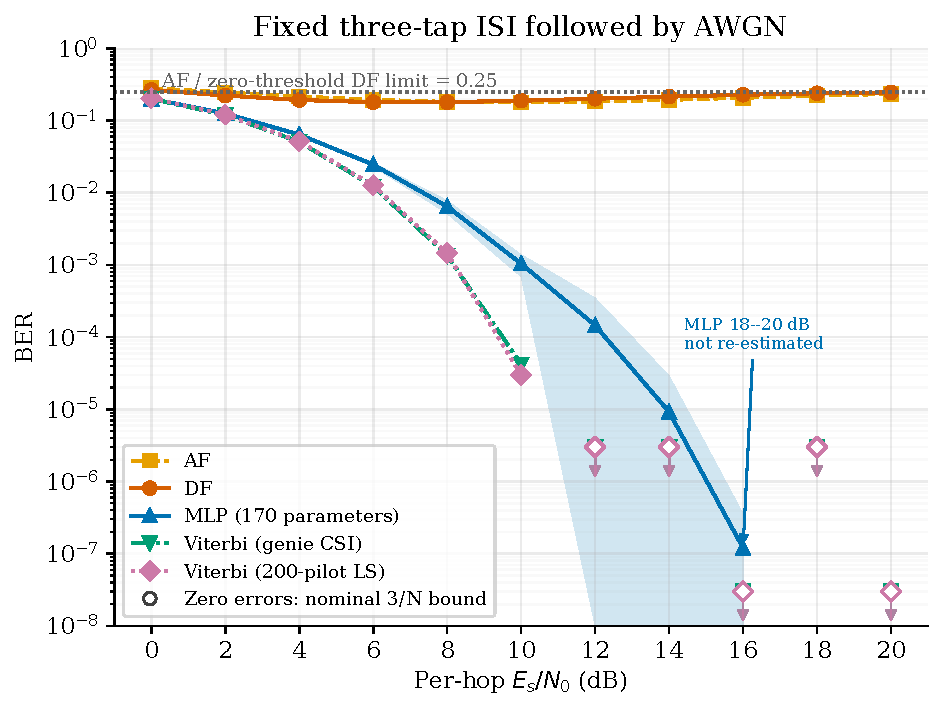
\includegraphics[width=\linewidth,height=0.39\textheight,keepaspectratio]{results/e6_unknown_channel.pdf}}
\caption[Unknown-channel relaying, fixed-budget validation through 16~dB]{Destination BER versus per-hop $E_s/N_0$. The original figure is regenerated with the same matched Viterbi sources as Table~\ref{tbl:tableE6}. MLP points above 16~dB are omitted. Open Viterbi markers show zero-error nominal $3/N$ bounds at the actual bit budgets, with downward arrows; these are not measured BERs. AF/DF/MLP bands use the stored across-checkpoint uncertainty at 12--16~dB and the historical intervals below 12~dB}\label{fig:figE6}
\end{figure}

\subsection{Does the Result Generalize to QPSK?}\label{sec:qpsk-unknown-channel}

The unknown-ISI study above uses BPSK throughout. The canonical setup of Chapter~\ref{sec:experiments} is QPSK, so this subsection asks whether the failure mode survives the move to that constellation. It is not a clean constellation control and is not offered as one: as Eq.~\eqref{eq:qpsk-hop1} below records, the QPSK study also puts an independent per-symbol fade on top of the fixed filter, so the two studies differ in channel as well as in modulation. Isolating the constellation would need a plain-QPSK-ISI run, which was not performed. The $0.25$ floor derived in Section~\ref{sec:unknown-channel-experiment} is a property of the \emph{binary zero-threshold} slicer: it counts the $2^{2}=4$ equiprobable interfering-symbol patterns that flip a $\pm1$ decision. It does not imply a QPSK symbol-error floor or a fixed QPSK BER, because QPSK decisions use two axes and this experiment also changes the fading model. The QPSK result is therefore a separate measured extension, not a direct theorem-level generalization. This subsection repeats the relay comparison with Gray-coded QPSK in place of BPSK, using the same nominal per-hop SNR axis ($\gamma=10^{\text{SNR}_{\text{dB}}/10}$) and the same relay families generalized to the complex alphabet: AF, symbol-wise DF (hard per-axis decision), a $193$-parameter $4$-class MLP-QPSK classifier (window 11, softmax cross-entropy, trained at SNR $\in\{5,10,15\}$ dB), and Viterbi MLSE generalized to the complex QPSK trellis ($4^{2}=16$ states, complex branch metrics).

One difference from the BPSK study matters more than it first appears. Hop~1 here is not the plain ISI channel of Section~\ref{sec:unknown-channel-experiment} but
\begin{equation}\label{eq:qpsk-hop1}
y[n] \;=\; g[n]\,(h * x)[n] \;+\; v[n], \qquad g[n] = |\,\mathcal{CN}(0,1)\,|\ \text{i.i.d.},
\end{equation}
an independent Rayleigh magnitude on every symbol on top of the fixed filter. A trellis built from $h$ alone is therefore \emph{not} a genie-CSI detector on this channel: its branch metrics compare $y[n]$ against unfaded expected values, leaving a residual $A^{2}(g[n]-1)^{2}$ that does not shrink as the noise does. Both detectors are reported below --- the taps-only trellis, and a genie-CSI trellis given $g[n]$ as well as $h$, which scales each branch's expected observation accordingly. Evaluation uses $10$ trials $\times$ $100{,}000$ bits per SNR point over the same $0$--$20$ dB range. No closed-form floor is derived for QPSK, so the curves below are reported as measured, not fit to a predicted asymptote. Because the QPSK relays are applied jointly to the complex signal rather than decomposed into two independent BPSK problems, and the per-relay power normalization is computed on total (I+Q) power, the resulting AF/DF operating points are not required to, and empirically do not, numerically match the BPSK figures of Table~\ref{tbl:tableE6} at the same SNR label; no such match is claimed.

\begin{longtable}[]{@{}llllll@{}}
\caption[QPSK unknown-channel BER (mean over 10 trials)]{QPSK unknown-channel BER (mean over 10 trials) on the per-symbol faded ISI channel of Eq.~\eqref{eq:qpsk-hop1}. AF and DF plateau at an elevated, non-monotonic BER across the SNR range tabulated, and the 193-parameter MLP-QPSK restores monotonically decreasing BER. The last two rows are the same trellis given different information: with the taps alone it is model-mismatched here and the MLP passes it above about 2~dB; given the per-symbol fading gains as well, it is the genie-CSI detector for this channel and leads the MLP everywhere.}\label{tbl:tableE6qpsk}\tabularnewline
\toprule\noalign{}
Setup & Relay & 8 dB & 12 dB & 16 dB & 20 dB \\
\midrule\noalign{}
\endfirsthead
\toprule\noalign{}
Setup & Relay & 8 dB & 12 dB & 16 dB & 20 dB \\
\midrule\noalign{}
\endhead
\bottomrule\noalign{}
\endlastfoot
QPSK: ISI $\to$ AWGN & AF & 0.2447 & 0.2116 & 0.2019 & 0.2100 \\
 & DF & 0.2197 & 0.2024 & 0.2074 & 0.2211 \\
 & \textbf{MLP-QPSK (193p)} & \textbf{0.1292} & \textbf{0.0827} & \textbf{0.0601} & \textbf{0.0508} \\
 & Viterbi (taps only) & 0.1307 & 0.0852 & 0.0670 & 0.0618 \\
 & \textbf{Viterbi (genie CSI)} & \textbf{0.0739} & \textbf{0.0155} & \textbf{0.0018} & \textbf{0.0001} \\
\end{longtable}

\begin{figure}[htbp]
\centering
\pandocbounded{\includegraphics[width=\linewidth,height=0.24\textheight,keepaspectratio]{results/unkchan_qpsk.png}}
\caption[QPSK unknown-channel relaying]{QPSK unknown-channel relaying, BER vs.\ SNR (10 trials, 100{,}000 bits/point). As with BPSK, AF and DF plateau far above the MLP and Viterbi curves. The MLP-QPSK curve separates below the \emph{taps-only} trellis beyond about 2 dB, but the correctly informed genie-CSI trellis (given the per-symbol fading gains as well as the taps) leads the MLP at every SNR, by a gap that widens with SNR}\label{fig:figE6qpsk}
\end{figure}

\textbf{Conclusion (QPSK with ISI and additional fading):} The evaluated QPSK experiment changes both the modulation and the channel, adding per-symbol Rayleigh magnitudes to the fixed ISI filter. Its results establish a benefit over the evaluated memoryless relays under that combined change. A plain-QPSK-ISI control with consistent $E_b/N_0$ accounting is required to isolate modulation order.

Two trellis detectors have to be distinguished on this channel, and Eq.~\eqref{eq:qpsk-hop1} is why. A trellis built from $h$ alone, on a channel that also fades per symbol, is model-mismatched rather than genie-informed, and its error rate flattens for that reason. Three controls on the same trellis (\texttt{qpsk\_trellis\_controls.py}, run under the exact configuration of Table~\ref{tbl:tableE6qpsk}) separate the two explanations at 20~dB: given the taps on the faded channel it reaches a symbol error rate of $0.113$; on the same channel with the fading removed, $0.000$; and given the fading gains as well, $0.0003$. The trellis is not at fault (it is verified never to return a path less likely than the transmitted sequence, and to reduce exactly to the nearest-symbol slicer when the ISI is removed) only its channel model was.

With the genie-CSI detector, the rounded destination BERs range from $0.3300$ against the MLP's $0.3389$ at 0~dB to $0.0001$ against $0.0508$ at 20~dB. The measured ordering agrees with the BPSK study, but the simultaneous modulation and channel changes prevent attributing that agreement to either factor alone.

The ordering is not an artefact of the error criterion either. A decomposition of the QPSK error events (\texttt{qpsk\_error\_decomposition.py}) separates the detectors on symbols as well as on bits: measured against the taps-only detector, the MLP is ahead on \emph{symbol} error rate as well from about 8~dB up ($0.0939$ against $0.1126$ at 20~dB), and the two lose almost the same number of bits per symbol error ($1.073$ against $1.090$), so the Gray map is not the route either. It cannot be, for a structural reason stronger than that measurement. The taps are real and the fading gain is a real magnitude, so $y[n] = g[n](h*x)[n] + v[n]$ separates into two independent real ISI channels carrying the in-phase and quadrature bits; conditional on the genie-supplied gains and taps, the symbol posterior therefore factorises into its I/Q bit marginals, and bit-wise MAP and symbol-MAP are the same detector on this channel, not merely close ones (\texttt{tests/test\_bcjr\_qpsk.py}, agreement to $5.6\times10^{-16}$).

At QPSK, the supplied-taps-and-gains Viterbi receiver substantially outperforms the 193-parameter MLP: the rounded destination BERs at 20~dB are $0.0001$ and $0.0508$. A precise multiplicative ratio should not be inferred from the rounded classical value. The supported benefit is relative to the tested memoryless baselines, not near-optimal BER. The relay-output BCJR control below addresses a different measurement endpoint.

\subsection{Relay-Output Control: BCJR/APP Against Viterbi MLSE}\label{sec:bcjr-benchmark}

Viterbi MLSE minimizes sequence error, whereas bit-MAP decisions minimize expected bit error under the supplied model \cite{BahlCockeJelinekRaviv1974BCJR}. The control in \texttt{qpsk\_bcjr\_benchmark.py} compares these two decisions with both taps and per-symbol fading gains supplied. It measures errors \emph{at the relay output before Hop~2}; Table~\ref{tbl:tableE6qpsk} measures destination errors. Thus this is not an end-to-end BCJR-versus-MLP experiment.

Two controls check the detector implementation. Removing fading while retaining ISI does not require MLSE and bit-MAP to agree: at 8~dB their BERs are $0.021764$ and $0.021424$, with paired difference $+0.00034\pm0.00016$, a resolved difference at the reported level. At 20~dB both record zero errors in $10^6$ bits; $3.0\times10^{-6}$ is a nominal independent-bit reference bound, not a proof of zero BER. Removing ISI is the appropriate exact-agreement control: BCJR reduces to the per-axis slicer on all $10{,}000$ tested symbols.

\begin{table}[htbp]
\centering
\caption[BER-optimal benchmark against Viterbi MLSE]{Genie-CSI Viterbi MLSE against the BER-optimal BCJR/APP detector on the same trellis, relay output, 10 trials of 100{,}000 bits. The interval is on the paired per-trial difference, $t(9,0.975)=2.262$}\label{tbl:bcjr-benchmark}
\begin{tabular}{rrrrl}
\toprule
SNR (dB) & Viterbi BER & BCJR BER & Relative gain & Paired 95\% CI \\
\midrule
0  & 0.250177 & 0.239113 & 4.42\% & resolved \\
4  & 0.162702 & 0.155861 & 4.20\% & resolved \\
8  & 0.068918 & 0.067245 & 2.43\% & resolved \\
12 & 0.015075 & 0.014857 & 1.45\% & resolved \\
16 & 0.001726 & 0.001725 & 0.06\% & includes zero \\
20 & 0.000127 & 0.000126 & 0.79\% & includes zero \\
\bottomrule
\end{tabular}
\end{table}

\textbf{Conclusion.} BCJR has no higher empirical relay-output BER at the sampled points; its paired advantage is not resolved at 16 and 20~dB. Bit-MAP optimality concerns expected loss under the model and does not guarantee ordering in every finite Monte Carlo sample. These controls support the local detector implementation. They neither establish an end-to-end BCJR margin against the MLP nor close the unmeasured BPSK bit-MAP comparison.

\subsection{A Fixed Composite Channel: Learned and Estimated-Model Relays}\label{sec:composite-channel}

This study cascades fixed three-tap ISI, a fixed saturating amplifier, and a randomly drawn block phase before additive noise, using DBPSK. It tests a combined impairment, not a factorial isolation of each cause. The implemented comparators are AF, differential detection, and pilot-LS Viterbi followed by differential decoding. The latter estimates a linear FIR model and is mismatched to the nonlinear amplifier; no claim that it is the strongest possible classical receiver is made. The 169- and 1{,}153-parameter MLPs are trained on this cascade family without receiving its analytic parameters at inference.

Evaluation uses 10 unique trials of 100{,}000 source bits per SNR and three trained MLP instances. Repeated classical seeds and the training/trial hierarchy prevent interpreting the historical plotting bands as independent-trial 95\% confidence intervals. They are retained only as descriptive bands. During this review, the composite AF path was found to add half the intended complex Hop~2 noise power. Its curve was rerun with the corrected variance, original ten unique trial seeds and bit budgets, recording errors, exposures and Student-$t$ intervals in \url{e6_unknown_channel_results/codex_composite_af_validation.json}. The other relays emit real signals and do not use the affected complex-noise branch; their stored point estimates are unchanged. Overlapping bands do not establish equivalence.

\textbf{Conclusion within this cascade.} AF and differential detection remain near BER $0.25$ at high SNR; this is an observation, not a derived universal floor for nonlinear channels. The 169-parameter MLP has much lower measured BER, reaching $2.5\times10^{-3}$ at 20 dB. Pilot-LS Viterbi has lower BER at 8~dB ($0.0674$ vs.\ $0.1073$ at 8 dB) and both round to $0.0025$ at 20 dB. Equal rounded values do not establish equivalent reliability. The larger MLP is also close at the last point, ending at a rounded $0.0025$ at 20 dB. Its mid-SNR means are lower than the small MLP's ($0.1016$ versus $0.1073$ at 8~dB; $0.0482$ versus $0.0542$ at 10~dB), but the historical intervals do not support a formal capacity-equivalence or paired-significance conclusion. These results support learned processing on this trained cascade family, not arbitrary impairment stacks, unseen channel families, or superiority over an optimally matched receiver.

\begin{figure}[htbp]
\centering
\pandocbounded{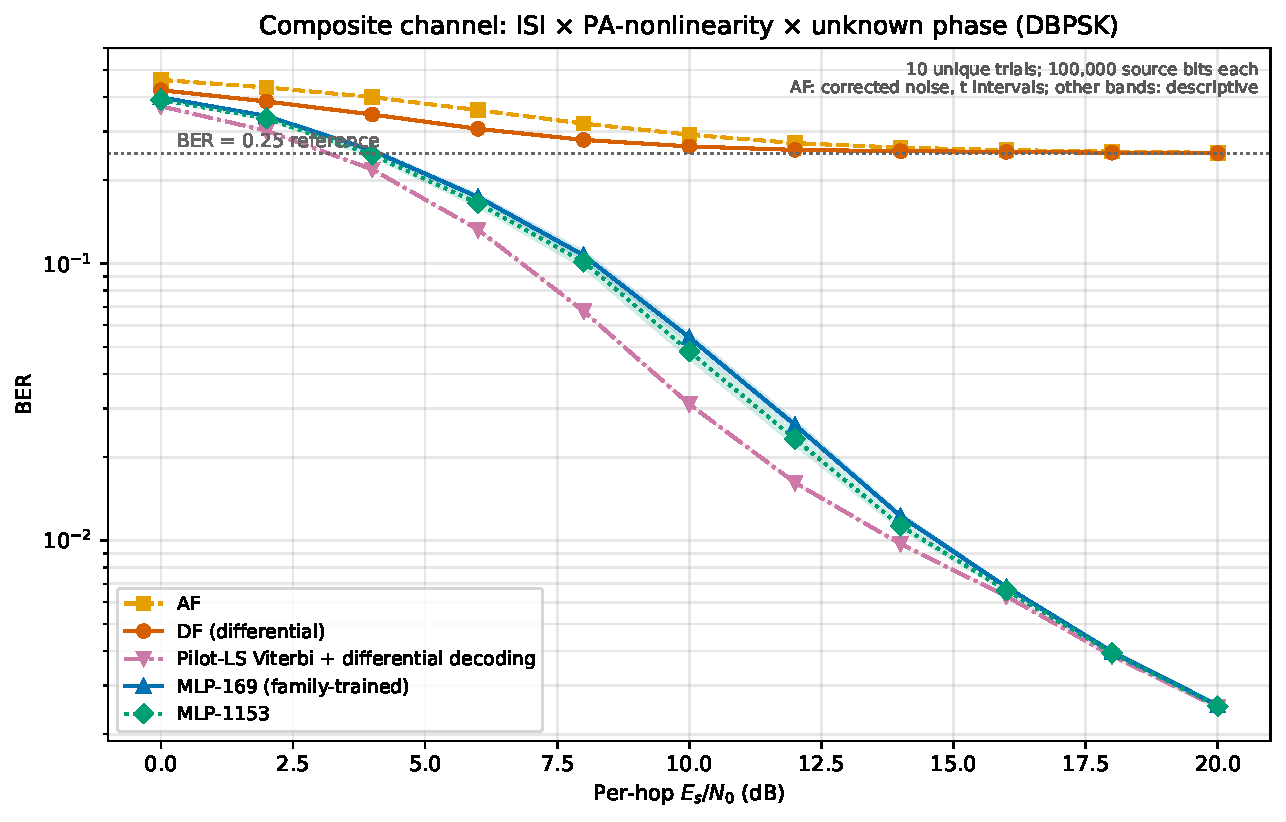
\includegraphics[width=\linewidth,height=0.36\textheight,keepaspectratio]{results/e6_composite.pdf}}
\caption[Composite multi-impairment channel]{Fixed ISI and amplifier with random block phase, DBPSK. The corrected AF curve uses ten unique fixed-budget trials and Student-$t$ intervals. Other curves retain historical point estimates and descriptive bands, which are not calibrated equivalence tests. Both MLPs were trained on this cascade family. Similar high-SNR rounded values do not demonstrate equal BER}\label{fig:figE6comp}
\end{figure}

\section{Layer 3 --- CSI Uncertainty: The Pilot-Budget Crossover}\label{sec:partial-posterior}

This is layer~3 of the ladder in Table~\ref{tbl:layers}: the pilot count is varied within the specified random composite-channel protocol. This differs from the preceding fixed-composite experiment. The pilot-aided trellis estimates a linear channel; it is not an oracle for the nonlinear cascade. Here channel information is limited: the pilot budget is finite, and the classical receiver must work from a correspondingly noisy estimate. Sweeping the pilot count on the composite channel at a fixed 10 dB operating point locates where the pilot-aided classical receiver ceases to beat the pilot-free learned relay, whose fixed trained estimator provides a horizontal reference (it uses no pilots at test). Its channel knowledge is amortized into its weights during training rather than estimated per block; the network is a discriminative estimator trained on the family, and its outputs have not been checked for calibration. \textbf{Evaluation:} 50 trials $\times$ 20{,}000 bits per operating point ($1{,}000{,}000$ bits), matching Section~\ref{sec:blind-channel} and for the same reason: the channel is redrawn per block, so trials are draws from the impairment family. In panel~(b) each trial is further subdivided into independent blocks of the swept length, so every block length is measured over the same total bit budget and over many channel draws rather than a single one.

\textbf{Conclusion (an estimation-variance cliff at 10 dB, and a rate--reliability tradeoff):} With a generous budget the classical partial posterior wins, as expected: pilot-aided Viterbi reaches payload BER $0.0285$ at 800 pilots and degrades only gently down to $0.0335$ at 20 pilots, comfortably below the MLP's pilot-free $0.0486$. At 10 pilots Viterbi has lost its edge, $0.0545$ against the MLP's $0.0486$, and at 5 pilots it reaches $0.1235$, because MLSE is then running on a badly estimated channel. The mechanism is estimation variance rather than rank deficiency: with 5 pilot observations and 3 complex taps the least-squares problem is formally overdetermined, but there are too few observations to average down the noise. The 95\% interval at that point is $0.1235 \pm 0.0304$, against $\pm 0.0011$ at 50 pilots. The MLP remains at $0.0486$ because it requires no per-block pilots after training on the channel family. Thus, at the measured 10-dB operating point, the crossover lies between 20 and 10 pilots. Its location is necessarily SNR-dependent because least-squares estimation error depends on noise power; no pilot-count sweep was run at another SNR, so a universal crossover is not claimed. The ordering is stable across the three trained MLP instances.

The practical force of this depends on block length, because a fixed pilot \emph{count} is a growing pilot \emph{fraction} as blocks shorten. Panel (b) sweeps block length at the same operating point with the classical receiver spending its minimum viable ten pilots per block, and adds blind CMA as the second pilot-free reference. The payload-BER confidence intervals overlap at the evaluated block lengths, both estimates being approximately $0.049$; the study has not established equivalence. At a 1000-symbol block the ten pilots cost $1\%$ of the block, whereas at a 40-symbol block, representative of low-latency or fast-varying links, they cost $25\%$, so the classical receiver carries data on only $75\%$ of the block against the learned relay's $100\%$ with no payload-BER difference detected at this budget.

Among the tested pilot-free methods, the fixed MLP has lower BER on these short blocks than CMA: CMA records $0.1723$ at $L=40$ and $0.1653$ at $L=1000$, versus its $0.0645$ long-block reference. This is consistent with limited adaptation time, but convergence failure is not isolated from other algorithmic settings. The MLP and pilot-aided receiver have no resolved difference at this budget; that is not proof of equal reliability. The conclusion is limited to the implemented baselines and block lengths.

\begin{figure}[htbp]
\centering
\begin{minipage}[t]{0.49\linewidth}\centering
  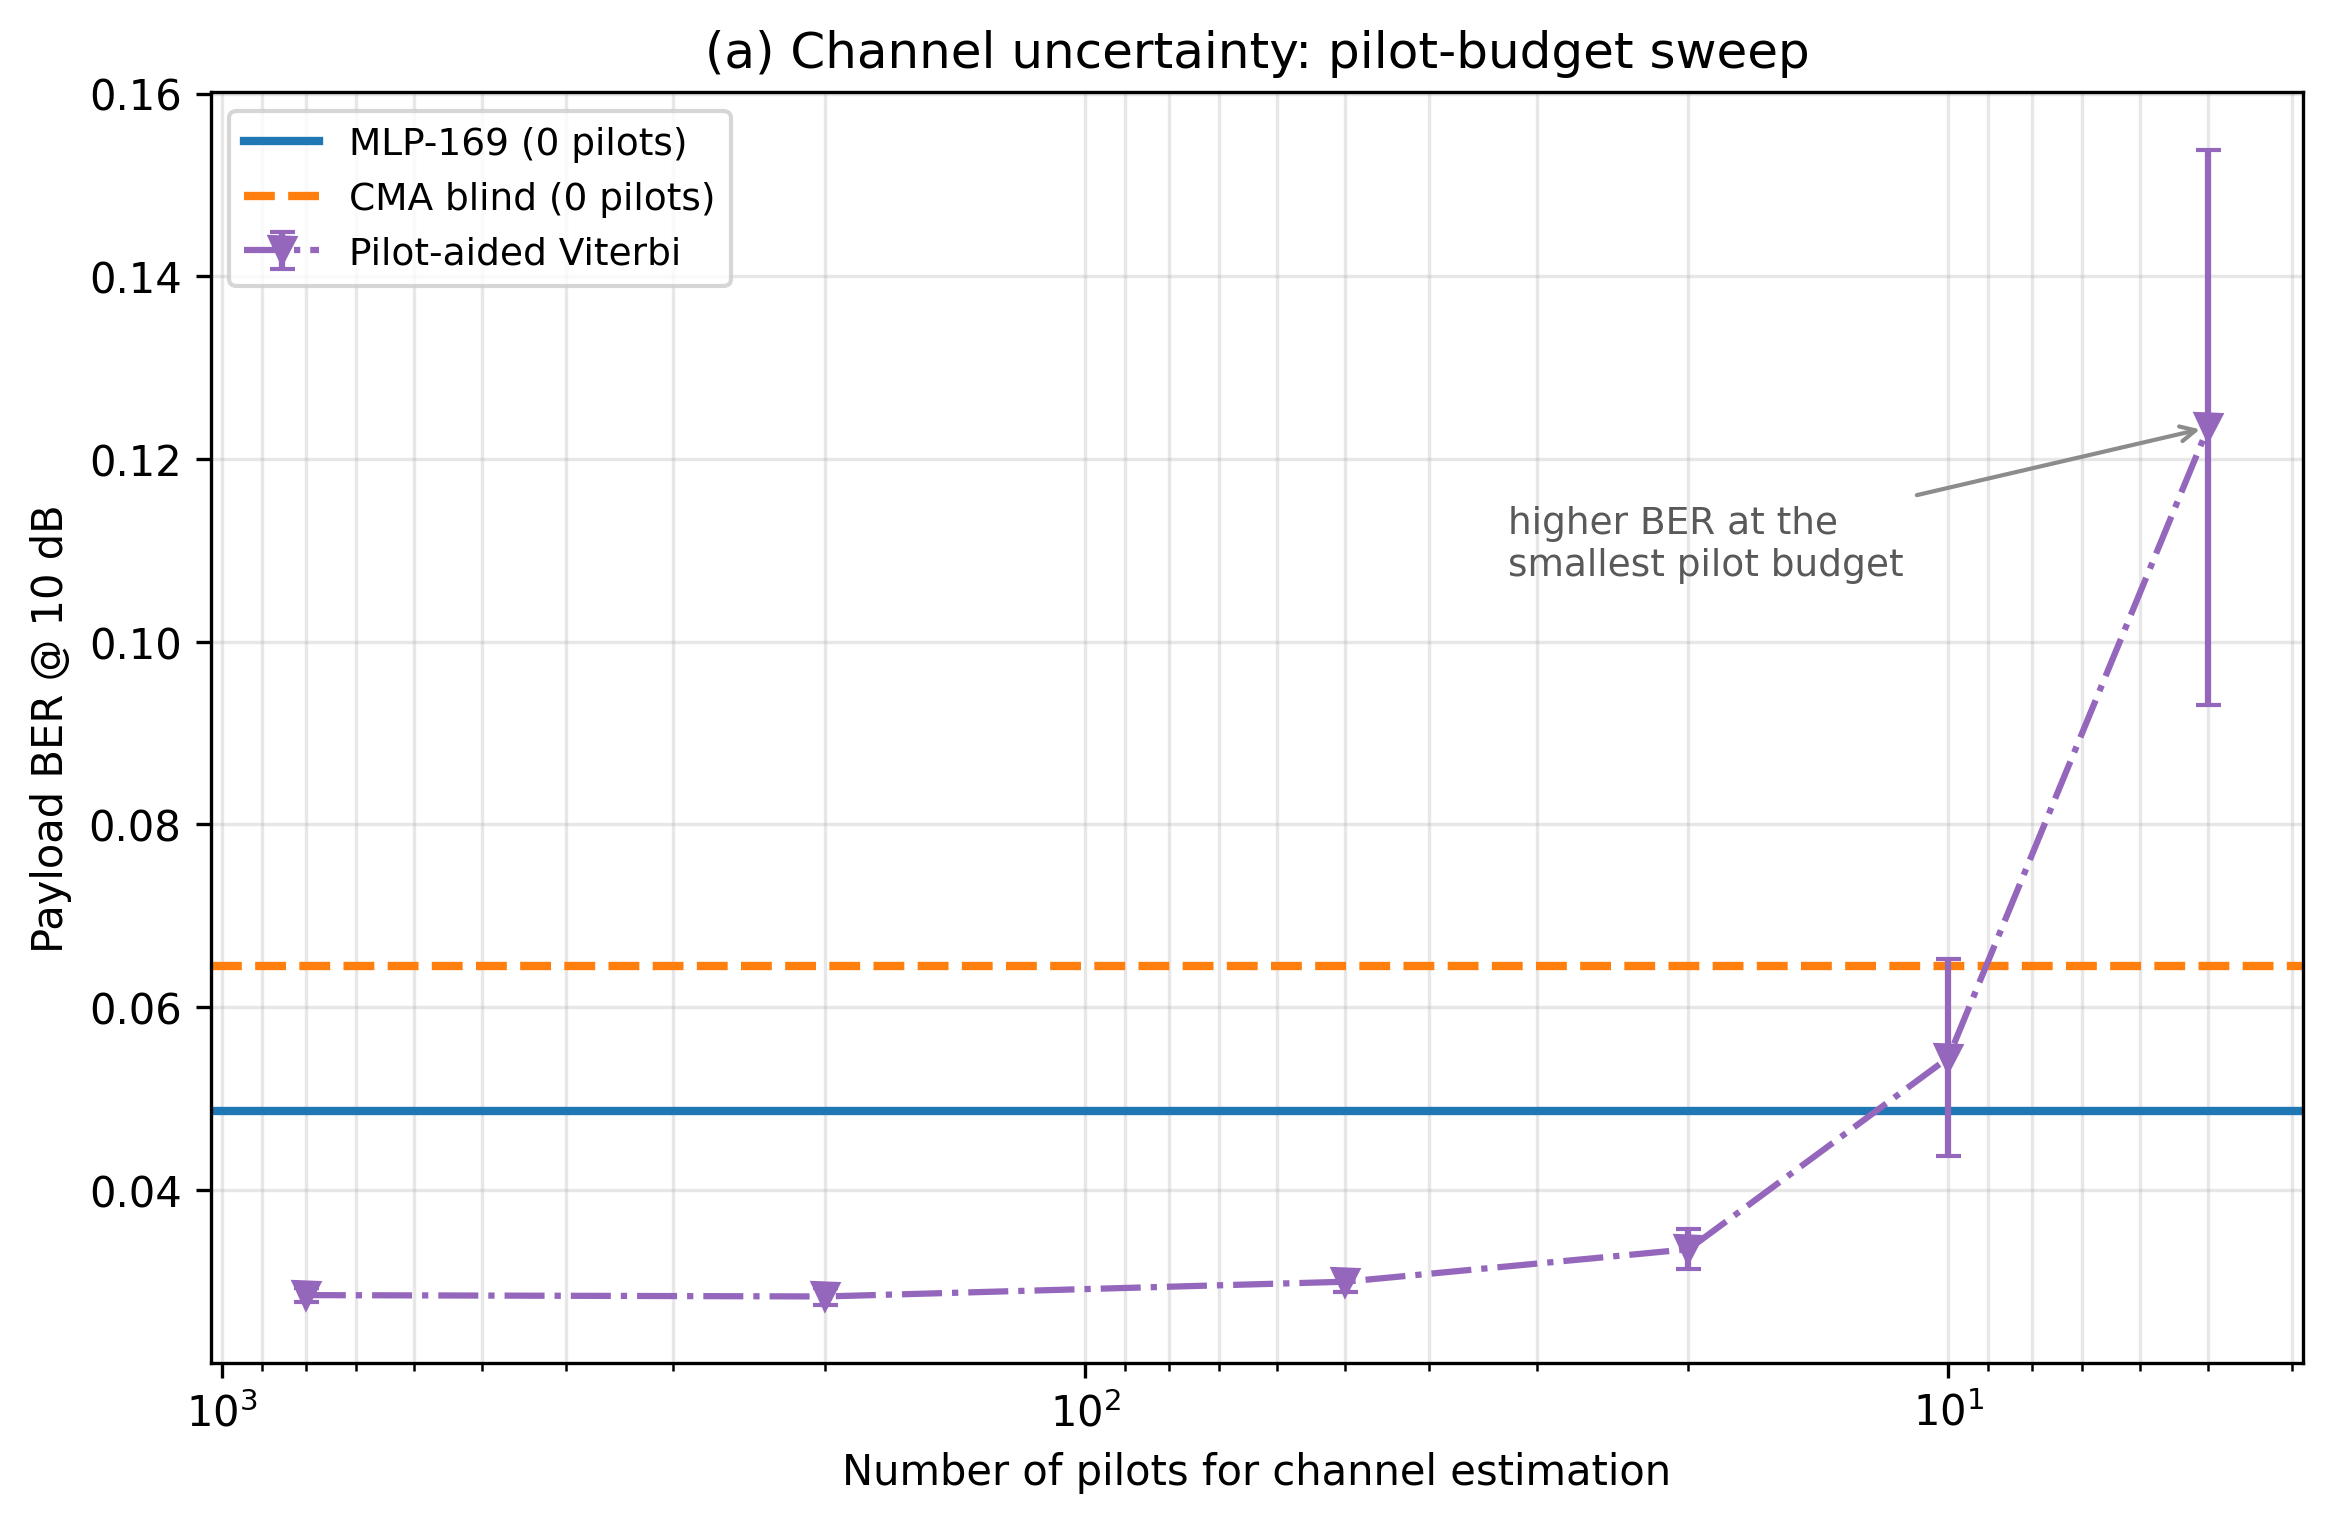
\includegraphics[width=\linewidth]{results/e6_partial_pilot_budget_sweep.png}\\[2pt]
  {\small (a) pilot-budget sweep at 10~dB}
\end{minipage}\hfill
\begin{minipage}[t]{0.49\linewidth}\centering
  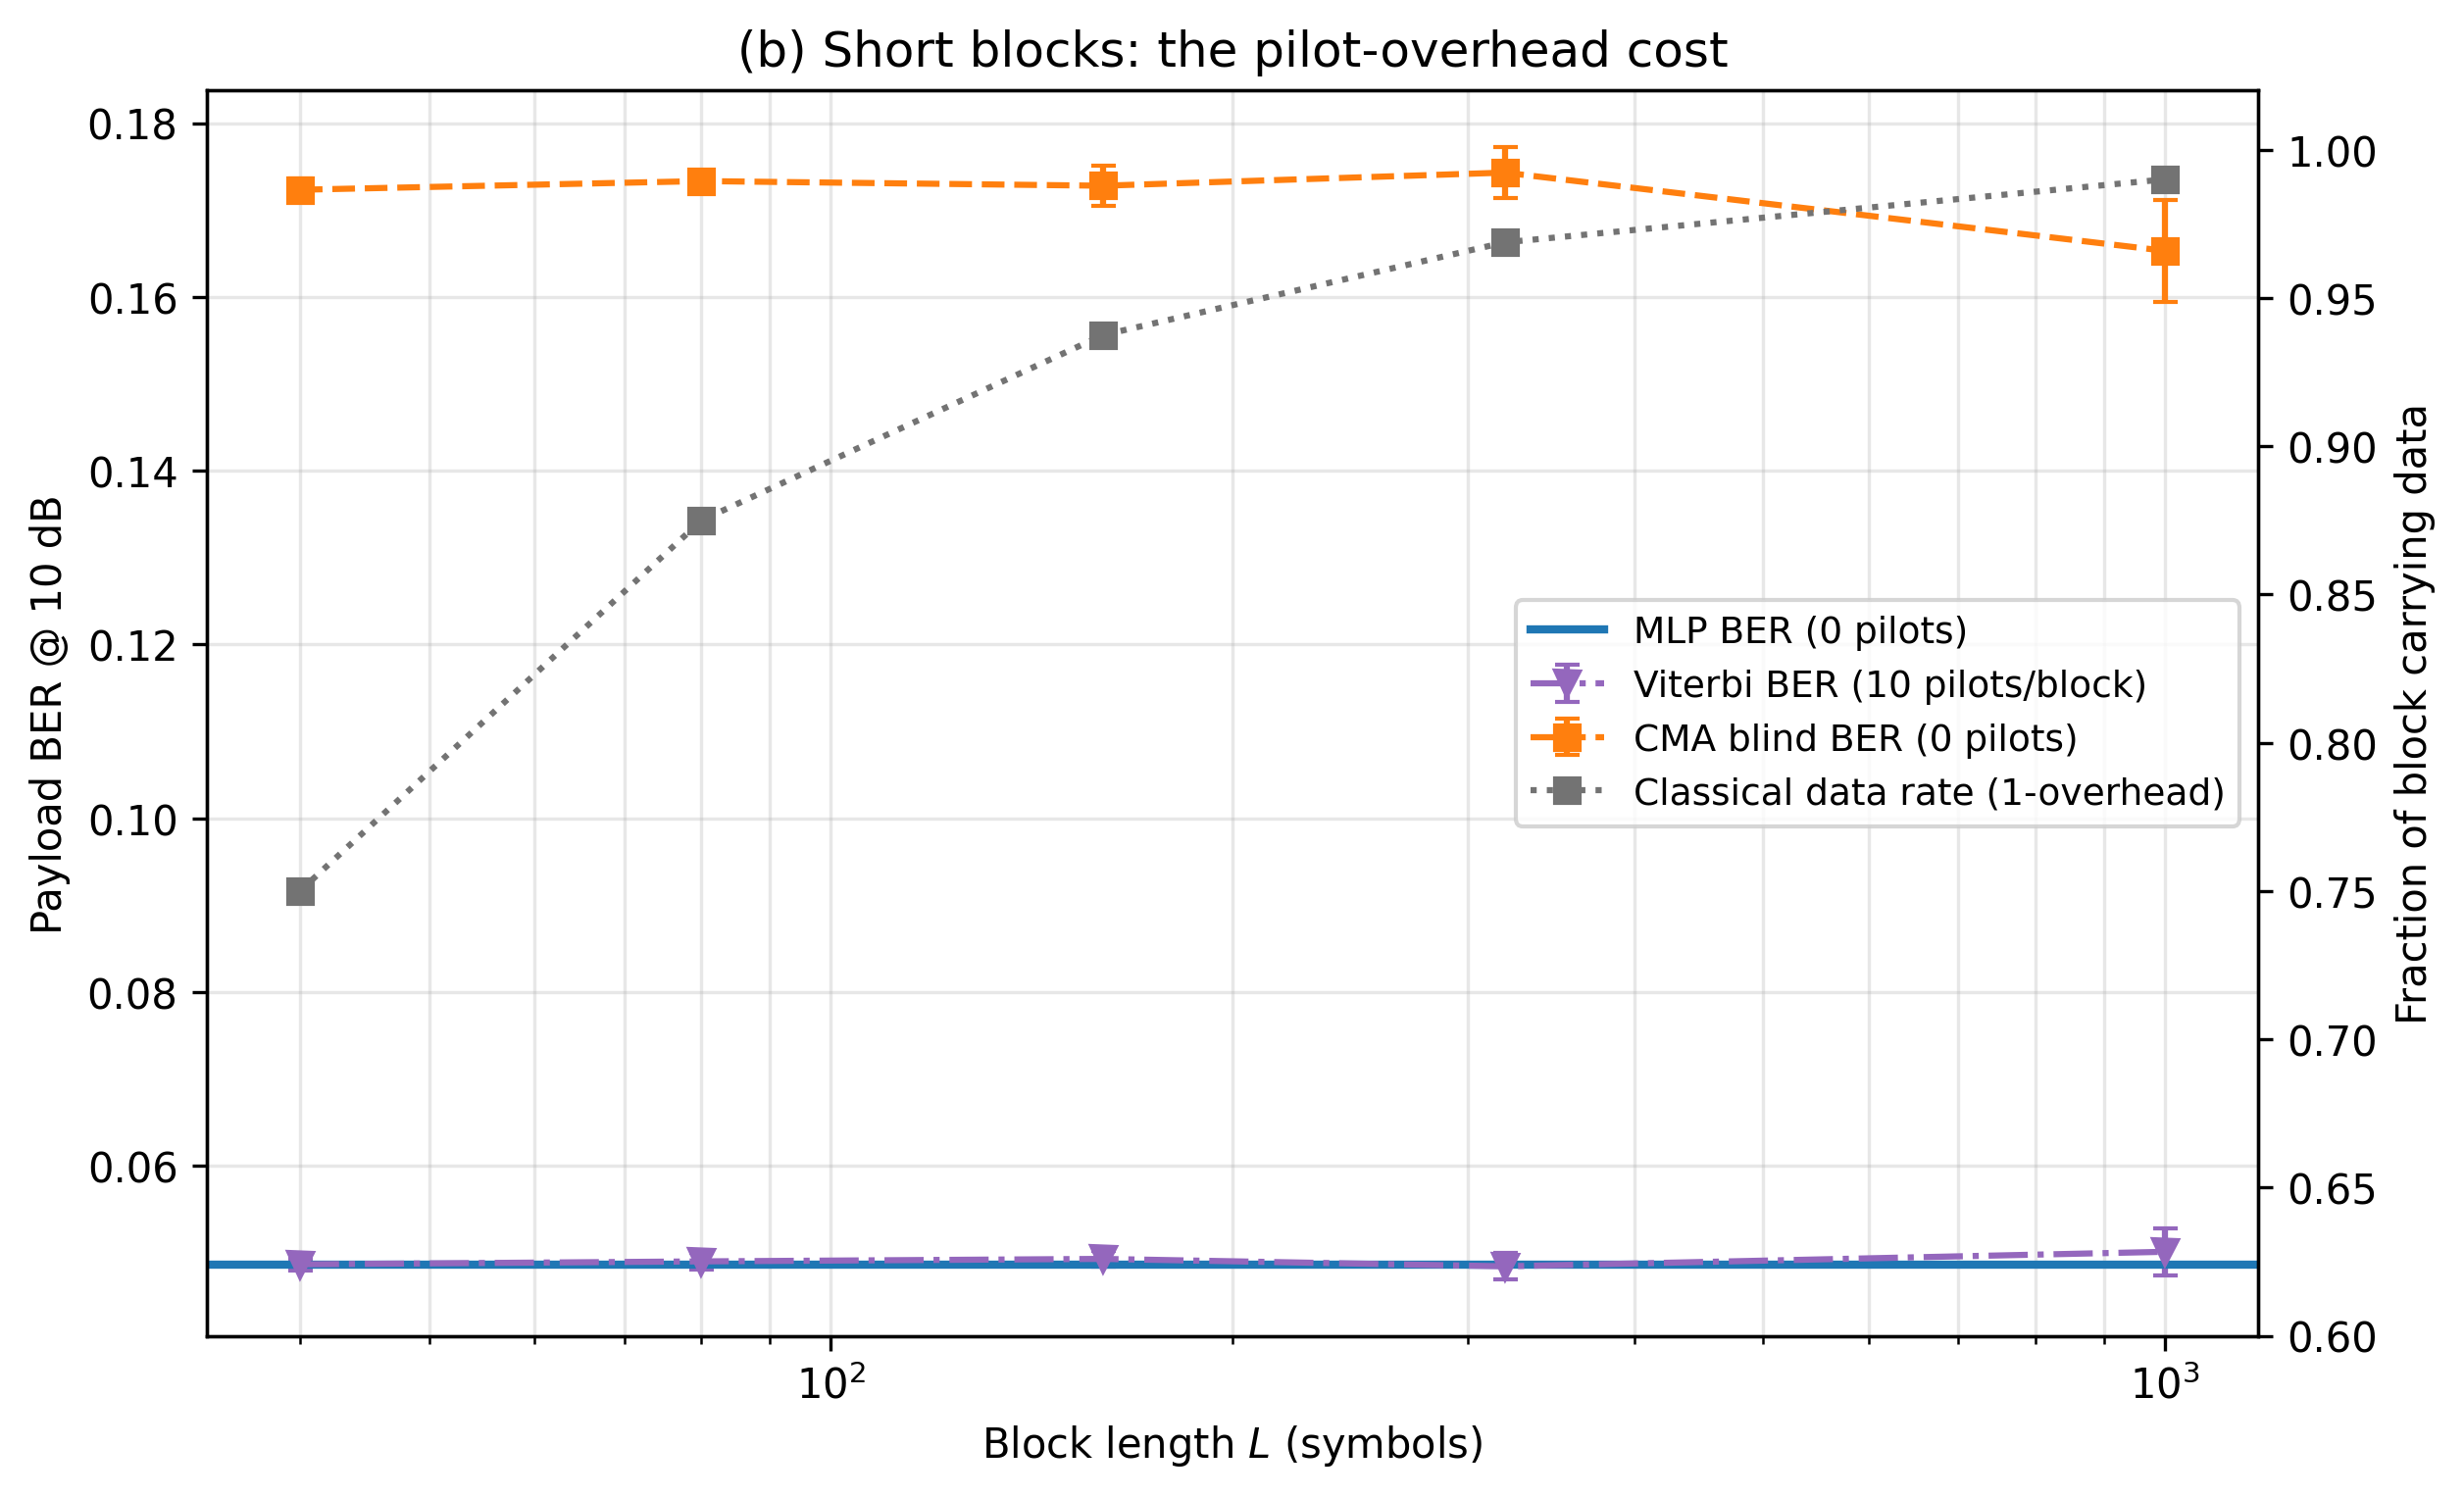
\includegraphics[width=\linewidth]{results/e6_partial_short_blocks_overhead.png}\\[2pt]
  {\small (b) block-length sweep at 10 pilots}
\end{minipage}
\caption[Finite-pilot sweeps: pilot budget and block length]{Finite-pilot regime; both panels are means over 50 channel draws at 20{,}000 bits/point. \textbf{(a)} Pilot-aided Viterbi outperforms the pilot-free MLP down to approximately 20 pilots per block, loses its edge by 10 pilots, and collapses at 5 pilots when the least-squares estimate becomes too noisy to construct a reliable trellis ($0.1235 \pm 0.0304$); the MLP is flat across the sweep, operating with a family-trained discriminative estimator and requiring no pilots. \textbf{(b)} With 10 pilots per block, pilot-aided Viterbi and the MLP have no detected payload-BER difference at the evaluated block lengths (both $\approx 0.049$), but the classical receiver's pilot overhead grows from approximately 1\% at $L=1000$ to 25\% at $L=40$. The tested CMA implementation has higher BER throughout. The MLP uses no pilots and has no resolved BER difference from the pilot-aided receiver at this budget; equivalence and superiority to untested pilot-free methods are not established}
\label{fig:e6_partial_pilot_budget}
\end{figure}

\section{Layer 4 --- Unknown Per-Block Realization: The Blind Regime}\label{sec:blind-channel}

This is layer~4, the bottom of the ladder. Per-block CSI and pilots are removed, and a fresh realization is drawn from the same impairment family used during MLP training. The comparison is against CMA, which assumes constant modulus and adapts an equalizer from the received block, and decision-directed MLSE, which bootstraps a channel estimate from its own decisions. Thus no method receives per-block CSI, but neither is assumption-free: the MLP knows the training distribution and CMA knows signal/equalizer structure. \textbf{Evaluation:} 50 independent channel draws $\times$ 20{,}000 bits per SNR point. Classical-method intervals use those 50 draws; neural uncertainty is assessed across trained instances rather than by treating repeated inference under one network as independent training evidence.

\paragraph{A correction to the blind equalizer.} The earlier fixed-step CMA implementation overflowed on longer blocks. The evaluated version normalizes its update by input-segment energy to limit this numerical instability. This is an implementation choice, not a proof that normalized CMA always converges or universally improves on fixed-step CMA. The results below concern the corrected implementation and its stated settings.

\textbf{Conclusion (learning narrowly leads CMA and avoids per-block adaptation):} The corrected CMA reaches BER $3.3\times10^{-3}$ at 20 dB, and the family-trained MLP reaches $2.6\times10^{-3}$. The MLP holds a small measured margin over the evaluated range, the MLP at $0.0955$ against CMA's $0.1182$ at 8 dB, while decision-directed blind MLSE is non-monotonic ($0.0374$ at 16 dB and $0.0498$ at 20 dB). Whether that margin is resolved is a question the intervals have to answer rather than the point estimates: the decision-directed MLSE interval at 8 dB is $\pm0.0201$, against the MLP's $\pm0.0026$ and CMA's $\pm0.0078$. This does not make CMA unstable: the observed instability belongs to the decision-directed MLSE implementation. CMA instead carries an online adaptation cost and requires enough samples to converge, whereas the MLP uses one fixed forward pass after offline training. For uncertainty reporting, the three trained MLP instances must be treated hierarchically rather than pooling their inference trials; classical methods have no training seed, so their effective sample size is the 50 independent channel draws. The supported conclusion is therefore narrow: on unseen per-block realizations from its training family, the MLP slightly outperforms the evaluated CMA implementation while avoiding per-block adaptation, and it avoids the non-monotonic behavior of the evaluated decision-directed MLSE.

\begin{figure}[htbp]
\centering
\pandocbounded{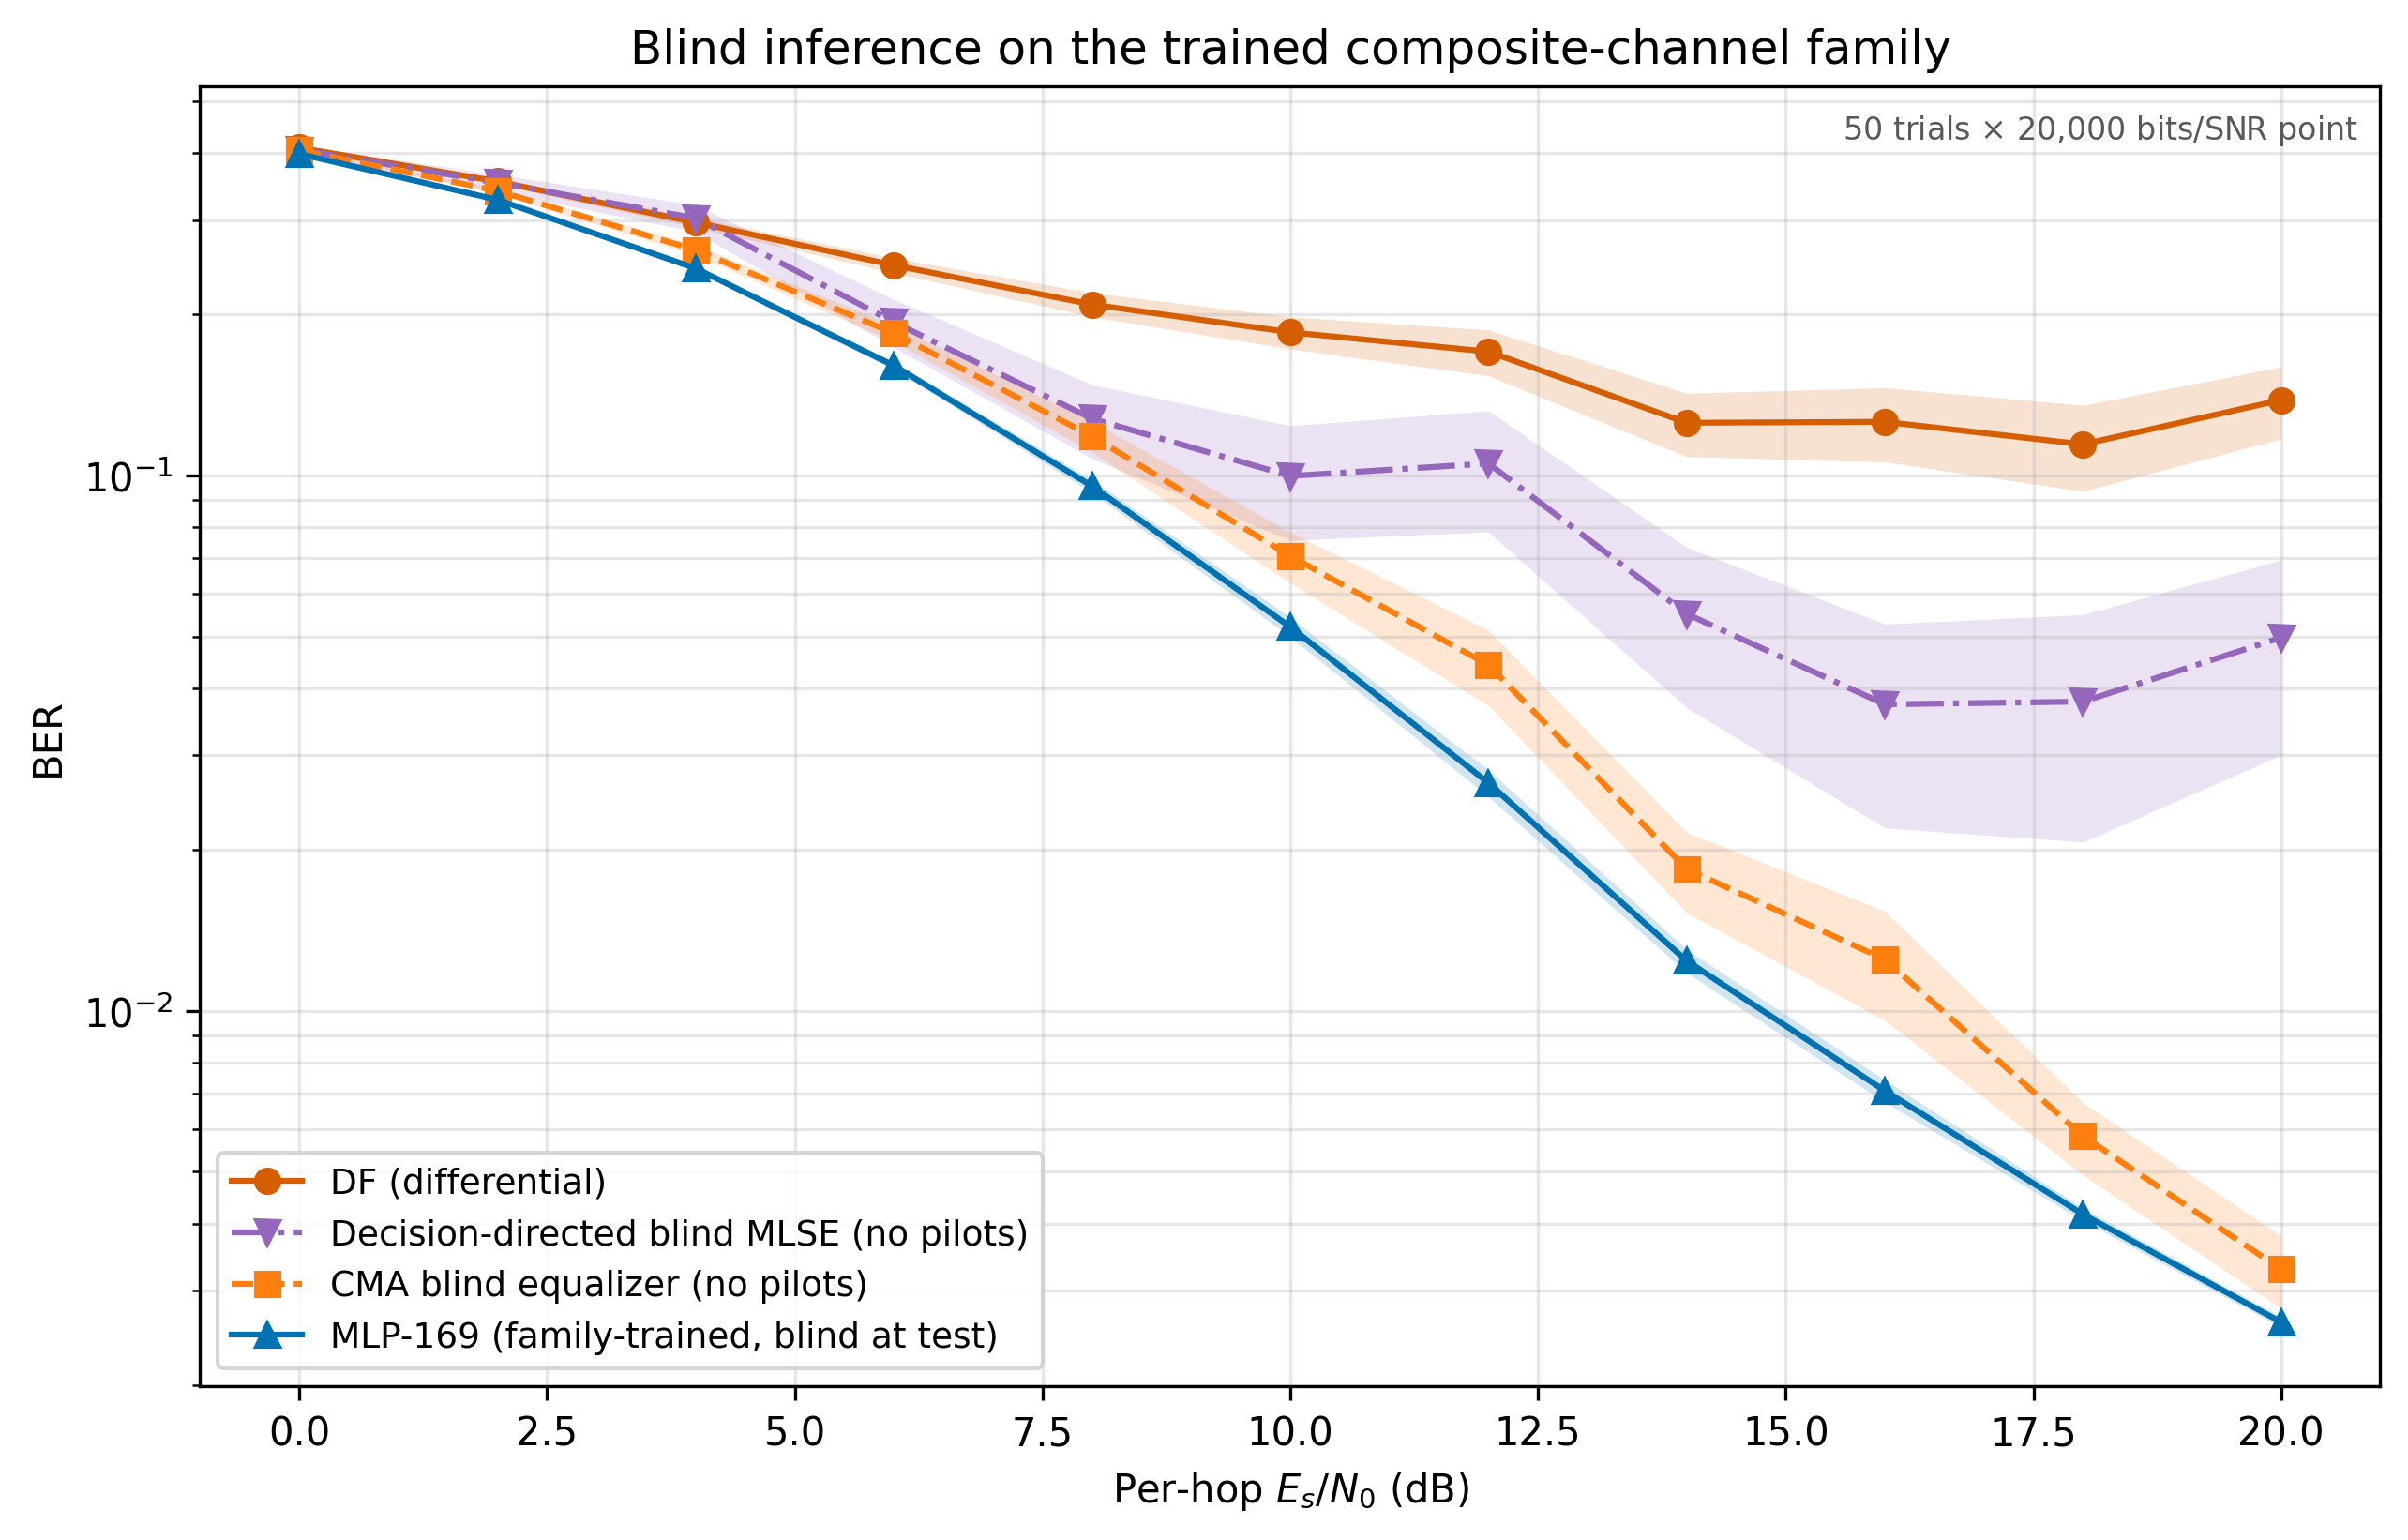
\includegraphics[width=0.82\linewidth,height=0.32\textheight,keepaspectratio]{results/e6_blind.png}}
\caption[Blind composite channel]{No pilots or per-block CSI; fresh realizations from the training family. The evaluated CMA and MLP means are close, while decision-directed MLSE has a non-monotonic high-SNR tail. Historical bands are descriptive; the neural training hierarchy prevents treating all pooled trials as independent confidence evidence. The MLP avoids test-time adaptation but uses family knowledge acquired in training. No claim against all blind equalizers is made}\label{fig:figE6blind}
\end{figure}

\subsection{A Low-Complexity Linear Baseline: MMSE Equalization}\label{sec:mmse-baseline}

The comparisons above set the learned relay against two classical relays, and neither is matched to it in cost. Symbol-wise DF is memoryless and cannot undo intersymbol interference at any transmit power, so outperforming it establishes only that the relay uses its window. Viterbi MLSE is the optimal sequence detector but costs $O(M^{L})$ per symbol in the channel memory, which is precisely the expense Section~\ref{sec:complexity-viterbi-mlp} invokes on the learned relay's behalf. The case between them was not tested: an $N$-tap MMSE linear equalizer is a natural low-complexity remedy an engineer might reach for before a trellis. If it recovered most of what the learned relay recovers, the contribution of Chapter~\ref{sec:unknown-channels} would be a narrower claim about a nonlinearity rather than about learned processing.

It does not. Table~\ref{tbl:mmse-baseline} gives the equalizer's SNR penalty against MLSE for equalizer lengths from 3 to 11 taps, measured on the same two-hop chains, with the exact channel taps supplied and the weights redesigned at every SNR point --- the same genie CSI granted to MLSE, and a longer window than the learned relay is given.

\begin{table}[htbp]
\centering
\caption[MMSE linear equalization against MLSE]{SNR penalty against Viterbi MLSE for an MMSE linear equalizer of $N$ taps, with the best learned relay on the same channel for comparison. Negative values beat MLSE. The reader should observe that the learned relay leads the equalizer by $1.8$ to $2.4$~dB on every channel, despite the equalizer being given exact channel knowledge, per-SNR weight redesign, and up to $11$ taps against the relay's window of $7$}\label{tbl:mmse-baseline}
\begin{tabular}{lrrrrr}
\toprule
Channel & 3 taps & 5 taps & 7 taps & 11 taps & Learned relay \\
\midrule
ISI (BPSK)      & $+6.58$ & $+4.40$ & $+4.23$ & $+4.04$ & $\mathbf{+1.67}$ \\
ISI (QPSK)      & $+7.81$ & $+9.11$ & $+5.02$ & $+4.84$ & $\mathbf{+3.03}$ \\
Composite       & $-0.33$ & $-0.37$ & $-0.37$ & $-0.44$ & $\mathbf{-2.26}$ \\
\bottomrule
\end{tabular}
\end{table}

The learned relay leads the tested linear-MMSE equalizers in the reported required-SNR metric. This is not a comparison against every cost-matched classical method; decision-feedback and reduced-state detectors were not evaluated. The MMSE decreases with filter length, as expected for nested linear estimators. BER and interpolated SNR penalties need not decrease with MSE, however. Consequently the non-monotonic QPSK penalty cannot be dismissed as an interpolation artifact without an additional check. The four-dB sampling grid is a further limitation on the precision of these penalties.

\subsection{Does a Sequence Architecture Help Where a Window Does?}\label{sec:sequence-on-memory}

Chapter~\ref{sec:experiments} finds that Transformer, Mamba-S6 and Mamba-2 buy nothing over a feedforward relay on the canonical channel, and attributes this to the channel rather than to the architectures: a memoryless channel offers no temporal structure for their inductive bias to exploit. That is a prediction about what would happen given such structure, and until now it was untested here, no sequence model having been evaluated anywhere in this chapter. The minimum-size study sharpens the prediction, finding the relay's \emph{window} to be the binding resource on channels with memory, worth $8$ to $11$~dB between window~1 and window~7 while width and depth buy almost nothing. A window is a blunt way of granting a feedforward network temporal context; sequence models are built for it.

The prediction fails. Table~\ref{tbl:seq-on-memory} compares the four architectures at an equal budget of approximately $3{,}000$ parameters, each trained on the channel under test rather than on a memoryless surrogate, with identical hyperparameters and three initializations apiece.

\begin{table}[htbp]
\centering
\caption[Sequence architectures on channels with memory]{SNR penalty against Viterbi MLSE at an equal budget of $\approx$3{,}000 parameters, with the across-initialization spread in brackets. Each entry is the \emph{best} of three initializations, not their mean, so the values are optimistic by construction and the comparison between architectures is only as sound as the bracketed spreads make it; the two Mamba variants' spreads here are wide enough that their ordering against each other should not be read as resolved. Negative values beat MLSE. The reader should observe that the feedforward relay leads every sequence architecture on every channel, and that the two Mamba variants (the most reproducible architectures measured on the canonical channel, at $0.019$ and $0.041$~dB) become the least reproducible here}\label{tbl:seq-on-memory}
\begin{tabular}{lrrrr}
\toprule
Channel & MLP-3K & Transformer-3K & Mamba-S6-3K & Mamba2-3K \\
\midrule
ISI (BPSK) & $\mathbf{+1.97}$ (0.39) & $+3.52$ (0.33) & $+4.30$ (1.15) & $+4.55$ (0.14) \\
ISI (QPSK) & $\mathbf{+2.58}$ (0.07) & $+5.96$ (0.45) & $+5.72$ (1.33) & $+4.69$ (2.12) \\
Composite  & $\mathbf{-2.08}$ (0.03) & $-1.76$ (0.03) & $-1.56$ (0.08) & $-1.60$ (0.06) \\
\bottomrule
\end{tabular}
\end{table}

For this equal-budget, shared-hyperparameter protocol, the feedforward relay has the best reported initialization on all three channels, by $1.55$ and $2.11$~dB on the two ISI cases and $0.32$~dB on the composite. Its observed training times are $35$--$66$~seconds per initialization versus $217$--$609$ for the sequence models. These results favor the tested windowed implementation; they do not establish that channel memory never benefits a tuned sequence architecture.

A second observation was not anticipated. The sequence models' reproducibility inverts. On the canonical channel Mamba-2 and Mamba-S6 are the two most stable architectures measured across initializations; on the complex ISI channel the same architectures spread by more than a decibel (bracketed spreads in Table~\ref{tbl:seq-on-memory}), while the feedforward relay stays inside $0.07$~dB throughout. They are worse on channels with memory, and substantially less predictable there, which compounds the case against them for this task.

One limitation is carried. All four architectures receive identical hyperparameters, matching the equal-budget protocol of Section~\ref{sec:parameter-normalization-complexity-trade-off}; no per-architecture tuning was attempted, and a tuned sequence model might close part of the gap.

\section{The Cost Side: Decision Delay and Arithmetic}\label{sec:complexity-viterbi-mlp}

The cost comparison distinguishes nominal arithmetic from measured implementation time. The BER tradeoff is configuration-dependent, and is not uniformly small, particularly in the QPSK study.

\textbf{Per-symbol cost and scaling.} MLSE maintains $M^{L-1}$ trellis states for a constellation of size $M$ and channel length $L$ (memory $L-1$), performing an add--compare--select over $M^{L}$ branch transitions per symbol; its cost therefore grows \emph{exponentially} in channel memory for fixed $M$, and polynomially in $M$ for fixed $L$. The 170-parameter MLP performs one fixed forward pass, about $330$ floating-point operations per symbol. That figure is a constant of the \emph{deployed} architecture, not a quantity independent of the channel: the input window has to span the memory, so its length grows with $L$, and the output dimension grows with the constellation, from a single real output at $M=2$ to the $193$-parameter QPSK relay used earlier in this chapter, and further still for denser constellations. Once those are fixed, the per-symbol cost is the same for every symbol and every channel realization, which is the property the comparison below relies on. The contrast with MLSE is therefore one of \emph{growth rate}, not of a constant against a variable: the network's cost rises roughly linearly in window length and output dimension, the trellis count is $M^{L}$.

For the studied BPSK three-tap channel, the nominal Viterbi count is about $64$ operations per symbol, below the MLP's approximately $330$ FLOPs (excluding activation-function cost). Full-state trellis counts grow rapidly for larger $M$ and $L$. A fixed network's arithmetic does not depend on the channel realization, but maintaining accuracy as channel complexity increases may require changing its window, width, or output dimension. Extrapolated operation counts for untested architectures are not evidence of retained BER or hardware speedup. Reduced-state sequence detection \cite{EyuboqluQureshi1988RSSE} and decision-feedback methods are unmeasured alternatives.

\begin{figure}[htbp]
\centering
\begin{minipage}[t]{0.49\linewidth}\centering
  \includegraphics[width=\linewidth]{results/e6_per_symbol_cost_vs_modulation_memory.png}
\end{minipage}\hfill
\begin{minipage}[t]{0.49\linewidth}\centering
  \includegraphics[width=\linewidth]{results/e6_right_clean.png}
\end{minipage}
\caption[Complexity: per-symbol cost and measured inference time]{Complexity of Viterbi MLSE against the 170-parameter MLP. \textbf{(a)} Per-symbol computational cost versus modulation order $M$ and channel memory $L$: Viterbi grows as $M^{L}$ (intractable by $M{=}16,L{=}5$), while the network grows only linearly in window length and output dimension ($\sim$330 flops for the deployed BPSK, $L{=}3$ relay). On the small studied channel (BPSK, $L{=}3$) Viterbi is actually cheaper; the MLP wins on \emph{scaling}, not on the small case. \textbf{(b)} Measured inference time for BPSK with $L=3$: the MLP is $30$--$90\times$ faster as a vectorized matmul versus Viterbi's interpreted sequential trellis scan}
\label{fig:figE6complexity}
\end{figure}

\textbf{Measured inference time.} For BPSK with $L=3$, the vectorized NumPy MLP is $30$--$90\times$ faster than the interpreted Python Viterbi implementation on the measured workload, despite Viterbi's lower nominal operation count. This includes implementation overhead. Optimized kernels and target-hardware throughput were not measured; no universal latency or hardware advantage is inferred.

\subsection{A Channel with Memory Under a Latency Constraint}\label{sec:joint-latency-memory}

The accounting above and the ladder that precedes it answer different questions and never meet. The ladder asks which detector is more accurate on a channel with memory, imposing no budget; this section's opening asks what each detector costs, without reference to a channel. What a deployment actually faces is both at once, and the two constraints do not have to bind in the same place. This subsection measures the intersection directly, and includes block DF, which the ladder omits: of the classical options it is the one whose cost is structural rather than arithmetic, so it is exactly the case the ladder's accuracy-only comparison cannot price.

Every scheme is placed inside one identical coded system so that the comparison is between relays and nothing else: a rate-$1/2$, $K=3$ convolutional code on QPSK, $200$ information bits per frame ($202$ symbols after tail), with soft Viterbi decoding of the code at the \emph{destination}. All schemes therefore deliver an information BER at the same information rate. Hop~1 carries the unknown $L$-tap ISI response ($h_k = 0.7^k$, unit-energy normalized) plus complex AWGN and hop~2 is AWGN; $150$ frames per trial and three seeds per point.

Each relay is then labelled with the structural decision delay it forces, in symbols: zero for AF and symbol-wise DF; $\lfloor W/2 \rfloor$ for a relay of window $W$, which must wait for the later half of its own window; $D$ for an MLSE with traceback depth $D$; and the full frame, $202$ symbols, for block DF, which cannot begin until the last symbol of a codeword has arrived.

\paragraph{No latency separation was resolved on the tested short-memory channel.} Table~\ref{tbl:joint-latency} gives the result at $L=3$. The BER at $12$~dB is unchanged at the reported precision from traceback depths $D=2$ through $D=15$. This finite-budget observation does not prove that all survivor paths merge by three symbols or that full-asymptotic accuracy is reached. Among the tested settings, MLSE at $D=2$ has less delay than the window-11 relay's five symbols and lower measured BER. Block DF spends $202$ symbols without a resolved accuracy gain in this experiment; with an equalizer it reproduces the reported MLSE value but adds frame buffering.

\begin{table}[htbp]
\centering
\caption[Relay cost and accuracy under a latency constraint]{Coded information BER at $12$~dB on the three-tap channel, against the structural decision delay each relay forces and its arithmetic per symbol. Mean of three seeds. No BER difference among the tested MLSE traceback depths is resolved at the reported precision; this is not an equivalence or survivor-merger test}\label{tbl:joint-latency}
\begin{tabular}{lrrr}
\toprule
Relay & Delay (symbols) & MACs/symbol & BER at $12$~dB \\
\midrule
AF                    & $0$   & $2$   & $0.0609$ \\
DF-hard (symbol-wise) & $0$   & $0$   & $0.3027$ \\
MLP $W=5$             & $2$   & $112$ & $0.0010$ \\
MLP $W=11$            & $5$   & $208$ & $0.000189$ \\
MLP $W=21$            & $10$  & $368$ & $0.000278$ \\
MLSE $D=2$            & $2$   & $128$ & $\mathbf{0.000033}$ \\
MLSE $D=3$            & $3$   & $128$ & $\mathbf{0.000033}$ \\
MLSE $D=15$           & $15$  & $128$ & $\mathbf{0.000033}$ \\
block DF              & $202$ & $16$  & $0.0411$ \\
block DF $+$ MLSE     & $205$ & $144$ & $0.000033$ \\
\bottomrule
\end{tabular}
\end{table}

The symbol-wise relays confirm the chapter's Layer~2 finding inside the coded chain: AF and hard DF do not merely lose, they fail, DF's BER \emph{rising} with SNR from $0.2913$ at $8$~dB to $0.4253$ at $20$~dB as the interference rather than the noise comes to dominate its decisions.

\paragraph{The cost convention.} Counts below are multiply--accumulates per transmitted symbol, stated here so they can be checked. Additions and comparisons carrying no multiply are excluded; they dominate the trellis search, so the comparison is conservative against this thesis's own conclusion. MLSE has $M^{L-1}$ states and $M$ branches from each, so $M^{L}$ branch metrics per symbol; with the expected observation precomputed each is $|y-c|^{2}$ on a complex difference, two real multiplies, giving $2M^{L}$ (its further $M^{L}$ additions and $M^{L-1}(M-1)$ comparisons are not counted). The relay's $2W$-value input window, the $I$ and $Q$ streams, into $H$ hidden units is $2WH$, and the four-class head $4H$, giving $2WH+4H$; biases are additions and the activations transcendental, so neither is counted.

\paragraph{Arithmetic at a fixed architecture.} With hidden width $H$ fixed, increasing the input window $W$ increases the stated network count linearly, whereas full-state MLSE grows exponentially in tap count $L$ at fixed constellation size $M$. No experiment establishes that fixed $H$ or a particular rule $W=O(L)$ preserves accuracy for arbitrary longer channels. Equating these counts gives an arithmetic crossover, not a universal performance boundary:
\begin{equation}
L^{\star} = \log_{M}\!\left(\frac{2WH + 4H}{2}\right) = 3.35 \text{ taps (MAC-count crossover)}
\label{eq:mac-crossover}
\end{equation}
for $W=11$, $H=8$ and $M=4$ ($2.90$ taps at $W=5$, $3.76$ at $W=21$). At three taps, MLSE's stated count is 128 versus the relay's 208; at seven taps the counts are 32{,}768 and 208. Table~\ref{tbl:joint-memory} reports measured BER separately. The crossover does not assert equal accuracy or a processor-independent speedup.

\begin{table}[htbp]
\centering
\caption[Cost and accuracy against channel memory]{Coded information BER at 12~dB and per-symbol arithmetic. MLSE has genie CSI and traceback $5L$; the 220-parameter window-11 relay is fixed. Measurements at $L=3,5,7$ use 1.5M information bits and five seeds; rows $L=4,6$ contain arithmetic only. Bracketed nominal 95\% Wilson intervals inherit the adjacent BER exponent; coverage under coded error correlations is not established. MLSE has lower measured BER throughout}\label{tbl:joint-memory}
\begin{tabular}{@{}p{0.04\linewidth}p{0.12\linewidth}p{0.14\linewidth}p{0.10\linewidth}p{0.23\linewidth}p{0.22\linewidth}@{}}
\toprule
$L$ & MLSE states & MLSE MACs & Relay MACs & MLSE BER (nominal CI) & Relay BER (nominal CI) \\
\midrule
$3$ & $16$      & $128$      & $208$ & $3.20\times10^{-5}$ \newline [2.41, 4.24] & $2.36\times10^{-4}$ \newline [2.13, 2.62] \\
$4$ & $64$      & $512$      & $208$ & ---                                     & ---                                     \\
$5$ & $256$     & $2{,}048$  & $208$ & $4.20\times10^{-5}$ \newline [3.28, 5.37] & $1.96\times10^{-4}$ \newline [1.75, 2.20] \\
$6$ & $1{,}024$ & $8{,}192$  & $208$ & ---                                     & ---                                     \\
$7$ & $4{,}096$ & $32{,}768$ & $208$ & $2.47\times10^{-5}$ \newline [1.79, 3.40] & $1.91\times10^{-4}$ \newline [1.70, 2.14] \\
\bottomrule
\end{tabular}
\end{table}

In the separately measured three-, five-, and seven-tap settings, the fixed architecture uses $208$ MACs per symbol. Its BER ranges from $1.91\times10^{-4}$ to $2.36\times10^{-4}$; overlapping intervals do not establish constant error or equivalence. The MLSE arithmetic count increases by a factor of $256$, while its measured BER advantage remains configuration-dependent. Under this counting convention, the fixed MLP crosses full-state MLSE in multiplication count between three and five taps. This is not a universal threshold or a guarantee of accuracy beyond the evaluated channels.

Two limits are worth recording. The threshold is a statement about \emph{arithmetic}, not about accuracy: above $L^{\star}$ MLSE remains the more accurate detector wherever it can be afforded, and the learned relay's case rests on it becoming unaffordable rather than on it becoming wrong. And the three-tap channel used throughout this chapter sits \emph{below} $L^{\star}$, so this chapter's earlier results should be read as establishing the failure of the memoryless relays on channels with memory, which they do, and not as a cost argument against MLSE, which at $L=3$ they cannot support.

Taken together, the studies show benefits of the tested learned relays over specified mismatched or memoryless comparators, with limitations from training-family dependence, finite budgets, and untested classical alternatives. They do not overturn the matched memoryless controls or establish a general superiority of learned relaying.

\chapter{Discussion and Conclusions}\label{sec:discussion-and-conclusions}

The canonical, coded, and unknown-channel studies answer related but distinct questions. Their channel models, architectures, endpoints and uncertainty units must not be combined into a single causal experiment. This chapter interprets their findings; Chapter~\ref{sec:summary} records the hypothesis outcomes.

\section{Interpretation of Results}\label{sec:interpretation-of-results}

\subsection{Low-SNR Advantage over AF (H1)}\label{sec:low-snr-advantage-of-neural-relays-h1-confirmed}

The evaluated feedforward relays have lower canonical BER than AF at 0--4~dB, supporting H1. At 0~dB the Hybrid, MLP and VAE means are $0.3329$, $0.3349$, and $0.3359$, compared with DF's $0.3337$ and AF's $0.4076$ (Table~\ref{tbl:table2}). The sequence models are closer to AF at that point. These are configuration-specific comparisons; model size alone does not explain them.

A nonlinear soft mapping is a plausible interpretation, not an isolated mechanism. For unit-energy BPSK in real AWGN, the posterior mean is $\tanh(y/\sigma^2)$, or $\tanh(2y)$ at $E_b/N_0=0$~dB. It minimizes local mean-squared error, not necessarily destination BER after relay normalization and Hop~2. The canonical QPSK/Rayleigh estimator also depends on fading reliability: after equalization, each real-axis variance is $N_0/(2|h|^2)$. If the relay function is not supplied $|h|$, it must implicitly average over that uncertainty.

The analytical CSI-assisted variable-gain AF expression $\gamma_1\gamma_2/(\gamma_1+\gamma_2+1)$ does not predict the block-normalized AF curve implemented here. Only the qualitative fact that linear amplification preserves noise alongside signal carries over.

\subsection{Medium-to-High-SNR Ordering (H2)}\label{sec:classical-dominance-at-high-snr-h2-confirmed}

DF matches or exceeds the evaluated learned relays from 6~dB upward. Coherent componentwise slicing is a local MAP symbol decision for the canonical channel, but that does not prove optimality among all power-constrained relay mappings for destination BER. Nor does tanh saturation isolate the cause of the learned models' finite-SNR penalties.

\subsection{Robustness Across the Sampled Ensemble}\label{sec:channel-robustness}

Training and testing use the specified Rayleigh distribution at sampled SNRs without online adaptation. This establishes performance over those draws, not every possible fade or an untested fading law. The equalization front end uses CSI even though the learned relay function receives no explicit channel coefficient.

\section{Capacity, Context and Training Variation}\label{sec:capacity-and-overfitting}
\label{sec:information-theoretic-perspective}

The original fixed-checkpoint comparison and later replicated sweeps are different experiments. The former finds the 169-parameter MLP competitive with much larger evaluated models; it cannot separate architecture from initialization and training. The replicated size sweep supports small configurations under its declared degradation criteria, but neither study measures the train/test decomposition needed to establish overfitting.

Under the canonical i.i.d.\ model, neighboring observations provide no additional information about the current symbol once the relevant current observation and side information are specified. That motivates a small mapping; it does not prove a minimum parameter count. On selected ISI channels, temporal context matters, but the smallest passing architecture is only the smallest found in the tested grid.

\subsection{Reading the Replicated Size Sweep}\label{sec:complexity-curve-turn}

The three-initialization sweep does not demonstrate the capacity-induced BER upturn proposed by H3. Its median across-initialization spread is $0.180$~dB across 152 configurations, but varies from $0.008$~dB on the canonical channel to $1.231$~dB on nonlinear bias. The pooled median is not a universal significance threshold. Two clusters of training outcomes do not by themselves identify optimization attractors or prove a mechanism.

Four-parameter configurations satisfy the zero-degradation criterion on three memoryless cases; selected three-tap cases use 73--145 parameters. These are empirical grid results, not architecture lower bounds. The coded size sweep spans 18--1{,}076 parameters with penalties of $+1.86$--$+1.92$~dB under its hard read-out. This motivates testing interfaces and metrics, but does not prove an interface-limited regime.

\subsection{Practical Implications}\label{sec:practical-implications}

The canonical 169-parameter model occupies 676 bytes of float32 weights. The BPSK fixed-ISI network instead has 170 parameters, and the coded-QPSK memory-sweep network has 220 parameters and 208 MACs per symbol. Their costs and results are not interchangeable. Parameter storage omits activations, input buffers, software and memory traffic; no embedded implementation, energy benefit, or sustained-throughput claim follows from it.

\section{Candidates for Further Deployment Evaluation}\label{sec:practical-deployment-recommendations}

\begin{longtable}{@{}p{0.27\linewidth}p{0.27\linewidth}p{0.39\linewidth}@{}}
\caption[Simulation-supported candidates]{Candidates suggested by the simulations, not hardware-validated recommendations}\label{tbl:table32}\\
\toprule
Tested regime & Candidate & Evidence boundary\\
\midrule
Canonical 0--4~dB & MLP/Hybrid and DF & Feedforward relays improve on AF; no general learned advantage over DF.\\
Canonical $\geq6$~dB & Symbol-wise DF & Lowest or tied-lowest evaluated BER; no training.\\
Selected ISI or uncertain-channel studies & Windowed MLP or model-based detector & Choice depends on the stated information, error target and cost. Family shift is untested.\\
\bottomrule
\end{longtable}

Hybrid switching uses the operating SNR and an empirical threshold. Threshold estimation error, quantization, synchronization and deployment robustness remain unmeasured.

\subsection{Latency and Adaptivity}\label{sec:latency-and-adaptivity-considerations}

Protocol scheduling, readiness and computation are separate costs. A symmetric window needs future samples; block decoding needs a frame; half-duplex forwarding still spends channel uses on both hops. Readiness may overlap the listening phase, but that is not a measured end-to-end latency saving.

In Section~\ref{sec:joint-latency-memory}, no BER difference is resolved among the tested traceback settings. A three-symbol MLSE setting has less look-ahead than the five-symbol windowed relay. The fixed network's multiplication count crosses the declared full-state MLSE count between three and five taps, while MLSE remains more accurate. This is an arithmetic comparison under the stated implementation convention, not a hardware latency crossover.

Neither the learned relay nor the canonical experiments demonstrate online adaptation. AF's gain is recalculated from block power, and DF requires no training; they must not be described as fixed-SNR baselines.

\section{Limitations}\label{sec:limitations}

\begin{enumerate}
\item \textbf{Experimental scope.} One two-hop SISO relay and no direct path are modeled. The canonical comparison uses uncoded QPSK; BPSK, DBPSK, faded-ISI QPSK and coded modulation studies are separate. The QPSK ISI re-check changes both modulation and fading. The 16-QAM coded grid is not a learned-relay architecture study.
\item \textbf{Model information.} Canonical receivers have perfect CSI. Pilot-limited and blind studies relax this within specified families. Training supplies family knowledge even when no analytic parameters or pilots are given at inference.
\item \textbf{Finite data and replication.} Fixed checkpoints, three-seed studies, paired trial tests and pooled-bit bounds have different uncertainty units. Nominal independent-bit intervals need not have their stated coverage under correlated decoding errors. Zero errors mean insufficient data for a positive BER estimate, not zero true BER. MLP fixed-budget ISI validation stops at 16~dB.
\item \textbf{Comparator scope.} Matched Viterbi optimizes sequence error. The QPSK bit-MAP control measures only relay-output BER, not destination BER. Reduced-state MLSE, decision feedback and fully reliability-weighted coded decoding are unmeasured alternatives.
\item \textbf{Coded metrics.} The implemented Viterbi and BCJR metrics omit symbol-dependent post-equalization reliability. The high-SNR ordering does not isolate quantization, consumed redundancy, or a general disadvantage of relay decoding.
\item \textbf{Generalization and hardware.} Memory is swept only through seven taps. New impairment families, correlated Doppler fading, other topologies, complete deadline models, quantized execution, energy and actual device timing are outside the evidence.
\end{enumerate}

\section{Future Work}\label{sec:future-work}

The most direct next controls are an end-to-end bit-MAP comparison with consistent information and power normalization, reliability-weighted coded metrics, and prospective training-seed replication. BPSK bit-MAP and plain-QPSK ISI would isolate questions left open by the present endpoint and modulation changes. Larger constellations require an appropriate multilevel output; a joint constellation classifier is one option, not a theoretical necessity for all separable QAM channels.

Other extensions include correlated time-selective fading, online adaptation, additional pilot SNRs, longer memories, reduced-state classical comparators, other codes and frame lengths, multi-relay/MIMO topologies, joint end-to-end learning, and measured hardware operation. These are proposals, not demonstrated capabilities.

\section{Hypotheses Revisited}\label{sec:conclusions}

H1 and H2 are supported within the canonical comparison. H3's overfitting explanation is not established. H4 does not hold across SNR: the low-SNR architecture gap persists, and the high-SNR convergence is not robust across all measured seeds. In the equal-budget replication, Mamba spreads are $0.019$ and $0.041$~dB, whereas the Transformer's is $0.906$~dB. These are three-seed observations, not universal architecture variances (Table~\ref{tbl:seed-spread-3k}).

Among eight Transformer initializations, one high-loss run has a much worse BER penalty. The all-run correlation is driven by that outlier. It motivates studying optimization failure, but does not establish a failure probability or validated screening rule; all runs remain in Appendix~\ref{sec:appendix-f-minimum-size}.

H5 is supported against the specified AF/DF and mismatched baselines in the evaluated settings. The matched BPSK required-SNR penalties vary from $0.26$ to $2.53$~dB with the target. Similar rounded BERs and overlapping intervals elsewhere do not establish equivalence. The coherent conclusion is bounded: small trained relays can help in particular mismatched pipelines, while model information, temporal context, decoder metrics and computational budgets determine the comparisons actually measured.

\chapter{Summary}\label{sec:summary}

This work examined classical and neural network–based relay strategies for \textit{two-hop relay communication} using a unified simulation framework. The objective was to analyze performance–complexity tradeoffs and determine when learning-based relays provide practical advantages over analytically derived methods.
The core comparison is carried out on one canonical setup, never departed from within it: a two-hop SISO link over i.i.d.\ Rayleigh fast fading, complex baseband, QPSK, uncoded BER, with the relay function as the only varied axis. The coded study and the unknown-channel contribution depart from it deliberately. The study showed the following:

\begin{enumerate}
    \item The best tested learned relays outperform AF at the evaluated low-SNR points (H1); the experiments do not isolate a unique mechanism for that advantage.
    \item Classical \textit{decode-and-forward (DF)} matched or outperformed all neural approaches at \textbf{medium-to-high SNR} while requiring no trainable parameters, confirming that DF is the best-performing evaluated symbol-wise classical relay in this regime (H2).
    \item Increasing model size did not produce a \textbf{systematic BER improvement}, and the replicated size sweep found no statistically meaningful upward BER trend attributable to model capacity (H3).
    \item The 169-parameter MLP is competitive with larger models in the original canonical comparison. This is not a universal minimum-size result, and no train/test-gap study establishes overfitting as the explanation.
    \item The replicated size sweep identifies the smallest tested configurations meeting each degradation criterion: four parameters suffice for three memoryless cases at zero degradation, while the selected three-tap cases use 73--145. Window length matters in this grid, but the experiment does not prove architecture lower bounds.
    \item At an equal parameter budget, feedforward and sequence relays remained separated at low SNR. The apparent high-SNR convergence was smaller than the Transformer run-to-run spread and is not seed-robust; equalizing parameters also left depth, width, state dimension, window, and optimization confounded (H4).
    \item Within the simulated benchmark, a \texttt{hybrid relay} combining neural processing at low SNR with DF at high SNR tracked the best evaluated relay when operating SNR was known. Its switching-threshold robustness, quantization, energy use, synchronization, and hardware behavior were not evaluated.
\end{enumerate}
    Findings 1--4 and 6--7 concern the canonical comparison; the size sweep spans several specified channel families. The following items summarize Chapter~\ref{sec:unknown-channels}. The supplementary coded study is summarized below.
\begin{enumerate}
\setcounter{enumi}{7}
    \item On the selected BPSK three-tap filter, AF and zero-threshold DF approach the derived $0.25$ floor, while the 170-parameter MLP substantially reduces BER through the fixed-budget 16-dB point. Matched genie MLSE leads over the resolved range; the interpolated required-SNR penalties are $0.26$, $1.18$, $1.88$, and $2.53$~dB at BER $10^{-1}$ through $10^{-4}$. These are not a constant offset. In the separate blind study, the family-trained MLP narrowly leads the evaluated CMA implementation without test-time adaptation.

    \item Sweeping the intermediate \emph{partial}-posterior case at 10~dB located a crossover between 20 and 10 pilots; its SNR dependence was not measured. Pilot-aided LS-plus-MLSE wins when its estimate is sufficiently accurate, while the family-trained relay avoids pilot overhead and per-block estimation. The result is specific to the tested estimator, channel family, block lengths, and SNR.

    \item The separate coded-QPSK memory sweep uses a window-11, eight-hidden-unit, four-output MLP with 220 parameters and 208 MACs per symbol. The nominal full-state MLSE count is $2M^L$ under the stated convention; the two counts cross between the evaluated three- and five-tap cases and differ by about $158\times$ at seven taps. MLSE remains more accurate. Fixed arithmetic is a property of this deployed network, not a guarantee that its accuracy or required size remains fixed for longer channel memories.

    \item \textbf{Latency did not separate the learned relay from sequence detection at the available resolution} on the tested channel. No BER difference was resolved among the tested traceback depths; a three-symbol MLSE setting had fewer symbols of decision delay than the window-11 relay's five. The block relay required a full frame before producing output and showed no resolved accuracy gain in this experiment. The two research objectives of Chapter~\ref{sec:research-objectives} therefore have boundaries set by different resources in the comparisons evaluated here --- channel-estimate reliability for the unconstrained question, arithmetic for the constrained one --- and the distance between them is a result rather than a restatement.
\end{enumerate}

\begin{longtable}[]{@{}
  >{\raggedright\arraybackslash}p{(\linewidth - 4\tabcolsep) * \real{0.3333}}
  >{\raggedright\arraybackslash}p{(\linewidth - 4\tabcolsep) * \real{0.3333}}
  >{\raggedright\arraybackslash}p{(\linewidth - 4\tabcolsep) * \real{0.3333}}@{}}
\caption[Hypothesis outcomes summary]{Research hypotheses, their statements, and experimental outcomes}\label{tbl:table33}\tabularnewline
\toprule\noalign{}
\begin{minipage}[b]{\linewidth}\raggedright
Hypothesis
\end{minipage} & \begin{minipage}[b]{\linewidth}\raggedright
Statement
\end{minipage} & \begin{minipage}[b]{\linewidth}\raggedright
Result
\end{minipage} \\
\midrule\noalign{}
\endfirsthead
\toprule\noalign{}
\begin{minipage}[b]{\linewidth}\raggedright
Hypothesis
\end{minipage} & \begin{minipage}[b]{\linewidth}\raggedright
Statement
\end{minipage} & \begin{minipage}[b]{\linewidth}\raggedright
Result
\end{minipage} \\
\midrule\noalign{}
\endhead
\bottomrule\noalign{}
\endlastfoot
H1 & Some AI relays outperform AF at low SNR & \textbf{Confirmed}: the best neural relays beat AF at 0--4 dB on the canonical channel \\
H2 & DF lowest-BER among per-symbol relays at high SNR & \textbf{Confirmed}: DF matches or beats all AI methods at \(\geq 6\) dB with 0 parameters \\
H3 & An error minimum at intermediate capacity & \textbf{Not supported in the tested range}. The replicated size sweep finds no robust BER upturn with capacity. No train/test-gap analysis establishes an overfitting mechanism; uncertainty is configuration-dependent \\
H4 & Equal parameter count makes architecture-dependent differences negligible & \textbf{Not supported across SNR}. Low-SNR differences remain; the apparent high-SNR convergence is not robust to all measured seeds. Width, depth, windows, state dimensions and optimization remain confounded \\
H5 & A small learned relay improves on AF and zero-threshold DF under the selected model mismatches & \textbf{Supported within the evaluated configurations}. The BPSK fixed-budget MLP reaches $1.20\times10^{-7}$ at 16~dB (36 errors in 300M bits), but does not establish an advantage over matched MLSE. QPSK has a substantial matched-MLSE advantage over the MLP. Pilot and blind results concern the specified impairment family, classical implementations, and budgets \\
\end{longtable}

The evidence supports targeted use of learned relays, not a general learned-versus-classical verdict. The measured advantages depend on model mismatch, available channel information, architecture, and budget. Reduced-state sequence estimation, decision-feedback equalization, and fully reliability-weighted decoding remain unmeasured alternatives.

The supplementary coded study reports a high-SNR reversal between learned forwarding and the implemented block-DF pipeline. Its decoder metrics ignore symbol-dependent post-equalization reliability, so the observations do not establish that decoding at a relay inherently wastes redundancy or must lose at high SNR. The rate-adaptation experiment compares two classical forwarding schemes on a finite modulation-and-coding grid; its goodput ordering and idealized buffering constraints are not a neural-relay deployment guarantee. Hardware timing, full half-duplex deadline accounting, other code families, and generalization outside the trained impairment families remain beyond the experiments.

% \include{chapters/equation_ref}
% \include{chapters/references}
\bibliography{chapters/references.bib}
\chapter{Appendices}\label{sec:appendices}
\section{Appendix B: Model Architectures and Hyperparameters}\label{sec:appendix-b-model-architectures-and-hyperparameters}

% column helpers
\newcolumntype{L}[1]{>{\raggedright\arraybackslash}p{#1}}
\newcolumntype{Y}{>{\raggedright\arraybackslash}X}

\begin{table}[ht]
\centering
\footnotesize
\setlength{\tabcolsep}{4pt}
\renewcommand{\arraystretch}{1.15}

\begin{tabularx}{\textwidth}{|L{2.1cm}|Y|L{3.2cm}|L{1.7cm}|L{2.3cm}|}
\hline
\textbf{Relay} &
\textbf{Network Topology} &
\textbf{Train Loss (LR)} &
\textbf{Total Params} &
\textbf{Implemen-}\\
\textbf{tation} \\
\hline
MLP (Minimal) &
Feedforward MLP, 5-symbol sliding window &
MSE, lr=0.01, 100 epochs &
169 &
NumPy (CPU) \\
\hline
Hybrid &
MLP + DF switching via learned SNR threshold ($\sim$5 dB) &
MSE (MLP only), lr=0.01 &
169 &
NumPy (CPU) \\
\hline
VAE &
Encoder--decoder latent model (7$\to$8$\to$1) &
$\beta$-VAE ($\beta=0.1$), Adam lr=$10^{-3}$ &
1{,}777 &
PyTorch (CUDA) \\
\hline
cGAN (WGAN-GP) &
Conditional GAN (generator + critic) &
WGAN-GP, Adam lr=$10^{-4}$ &
2{,}946 &
PyTorch (CUDA) \\
\hline
Transformer &
2-layer encoder, 4 heads, $d_{\text{model}}=32$ &
MSE, Adam lr=$10^{-3}$ &
17{,}697 &
PyTorch (CUDA/CPU) \\
\hline
Mamba-S6 &
Selective SSM, 2 S6 layers &
MSE, Adam lr=$10^{-3}$ &
24{,}001 &
PyTorch (CUDA/CPU) \\
\hline
Mamba-2 SSD &
Selective SSM with SSD kernel (2 layers) &
MSE, Adam lr=$10^{-3}$, clip=1.0 &
26{,}179 &
PyTorch (CUDA) \\
\hline
\end{tabularx}

\caption[Relay models, objectives and parameter counts]{Comparison of relay models, training objectives, parameter counts, and implementations}
\label{tab:relay_comparison}
\end{table}

\section{Appendix C: Reproducibility}\label{sec:appendix-c-software-architecture}

\subsection{Testing} The simulation framework carries 187 automated pytest tests covering channels, modulation, relay strategies, simulation, and statistics. In the recorded environment, the full suite passed; with PyTorch unavailable, 183 passed and four checkpoint-dependent tests were skipped.

\subsection{Reproducibility} Evaluation seeds are controlled for source-bit and noise generation. Training initialization was not consistently seeded for every original sequence-model checkpoint, so exact retraining of those models is not guaranteed; the later replicated sweeps report training-seed variation explicitly.

\paragraph{Provenance of the reported results.} Each reported result is associated with an experiment artifact and a verification script in the source-code repository, using the experiment-specific budgets documented in the relevant section and ledger. Independent audit requires that repository at the archived revision identifier; the ledger below documents the claimed provenance but cannot by itself reproduce every table cell.

\clearpage

\section{Appendix D: Master Experiment Ledger}\label{sec:appendix-e-master-experiment-ledger}

This ledger links major studies to their experiment artifacts. The table verifier checks a declared subset of numerical cells, not every number or figure. Historical \texttt{e6\_*.npy} paths are relative to \url{e6_unknown_channel_results/}; the central ISI figure and table additionally use the matched-protocol and fixed-budget companion files listed below.

{\footnotesize
\begin{longtable}[]{@{}p{0.18\linewidth}p{0.10\linewidth}p{0.12\linewidth}p{0.12\linewidth}p{0.36\linewidth}@{}}
\caption[Master experiment ledger]{Master experiment ledger: modulation, channel, and result-file provenance for every major study}\label{tbl:ledger}\tabularnewline
\toprule\noalign{}
Study & \shortstack[l]{Modu-\\lation} & Channel & Tbl/Fig & Result source \\
\midrule\noalign{}
\endfirsthead
\toprule\noalign{}
Study & \shortstack[l]{Modu-\\lation} & Channel & Tbl/Fig & Result source \\
\midrule\noalign{}
\endhead
\bottomrule\noalign{}
\endlastfoot
Canonical benchmark & QPSK & Rayleigh & tbl:2, fig:10 & \url{results/modulation/qpsk_rayleigh.json} \\
Normalized 3K-param.\ comparison & QPSK & Rayleigh & tbl:8 & \url{results/normalized_3k/3k_rayleigh.json} \\
Coded block-DF, $K$-sweep & QPSK & Rayleigh & tbl:34, 35 & \url{results/coded_df_experiment.json} \\
Coded high-SNR paired re-test & QPSK & Rayleigh & tbl:37 & \url{results/coded_high_budget_test.json} \\
Coded relay-error mechanism & QPSK & Rayleigh & tbl:38 & \url{results/coded_error_mechanism.json} \\
Coded soft-decision relaying & QPSK & Rayleigh & tbl:39 & \url{results/coded_soft_decision.json} \\
Equal-throughput \& latency & QPSK, 16-QAM & Rayleigh & tbl:40, 41 & \url{results/coded_latency_throughput.json} \\
Adaptive modulation/coding (AMC) & QPSK, 16-QAM & Rayleigh & tbl:42 & \url{results/coded_rate_adaptation.json} \\
Capacity under a latency budget & QPSK, 16-QAM & Rayleigh & tbl:43 & \url{results/coded_latency_capacity.json} \\
Unknown ISI (layer 2) & BPSK & AWGN (Hop 2) & tbl:E6 & Historical AF/DF/MLP below 12~dB: \url{e6_sim_ported_results.npy}; fixed-budget companion \url{codex_isi_fixed_budget_validation.json}; Viterbi: \url{results/e6_matched_protocol.json} and \url{results/e6_matched_highsnr.json}. \\
Flat-channel control & BPSK & Rayleigh & tbl:E6flat & \url{e6_flat_ported_results.npy} \\
Unknown ISI, QPSK generalization & QPSK & AWGN & \shortstack[l]{E6\\QPSK} & \url{e6_qpsk_unknown_channel_results.npy} \\
Composite impairment cascade & DBPSK & Rayleigh & \shortstack[l]{E6\\composite} & \url{e6_composite_ported_results.npy}; AF replaced by \url{codex_composite_af_validation.json}. \\
Partial posterior (pilot sweep) & BPSK & Rayleigh & E6partial & \url{e6_partial_ported_results.npy} \\
Blind channel (layer 4) & BPSK & Rayleigh & E6blind & \url{e6_blind_ported_results.npy} \\
Four-layer summary & mixed (above) & mixed (above) & tbl:layers & combination of the above \\
\end{longtable}
}

The result files above are themselves generated by named, committed scripts (e.g.\ \url{coded_rate_adaptation.py} produces \url{coded_rate_adaptation.json}); the correspondence between script and output file is one-to-one and is not separately tabulated here since the filenames make it explicit.

\begin{center}\rule{0.5\linewidth}{0.5pt}\end{center}

%% ── Hebrew Abstract (Back Matter) ───────────────────────────

\section{Appendix E: Minimum Relay Size and Initialization Variance}\label{sec:appendix-f-minimum-size}

Supporting material for the minimum-size study of Section~\ref{sec:minimum-relay-size} and the initialization-variance measurements discussed in Section~\ref{sec:capacity-and-overfitting}. The findings themselves are stated in those sections; what follows is the underlying tabulation and the figures, collected here to keep the experiment and discussion chapters to their conclusions.

\begin{longtable}[]{@{}llllllll@{}}
\caption[Smallest relay per degradation budget]{Smallest relay meeting a given degradation budget against each scenario's own published relay (MLP-169, or MLP-756 for the coded row), written as parameters and window. Most memoryless rows settle at window~1, but flat gain and nonlinear bias require wider windows at the strictest budget; every evaluated three-tap row requires window~5 or~7 until a full decibel is conceded. A dash indicates that no smaller configuration meets that budget}\label{tbl:table-minsize}\tabularnewline
\toprule\noalign{}
Channel & Taps & $\le$0~dB & $\le$0.1~dB & $\le$0.25~dB & $\le$0.5~dB & $\le$1~dB & $\le$2~dB \\
\midrule\noalign{}
\endfirsthead
\toprule\noalign{}
Channel & Taps & $\le$0~dB & $\le$0.1~dB & $\le$0.25~dB & $\le$0.5~dB & $\le$1~dB & $\le$2~dB \\
\midrule\noalign{}
\endhead
\bottomrule\noalign{}
\endlastfoot
awgn & 1 & 4p w1 & 4p w1 & 4p w1 & 4p w1 & 4p w1 & 4p w1 \\
rayleigh & 1 & 4p w1 & 4p w1 & 4p w1 & 4p w1 & 4p w1 & 4p w1 \\
flat gain & 1 & 21p w3 & 21p w3 & 21p w3 & 4p w1 & 4p w1 & 4p w1 \\
branch asym. & 1 & 4p w1 & 4p w1 & 4p w1 & 4p w1 & 4p w1 & 4p w1 \\
nonlinear bias & 1 & 29p w5 & 4p w1 & 4p w1 & 4p w1 & 4p w1 & 4p w1 \\
ISI & 3 & 73p w7 & 73p w7 & 57p w5 & 57p w5 & 37p w7 & 21p w3 \\
ISI (complex) & 3 & 73p w7 & 73p w7 & 73p w7 & 73p w7 & 57p w5 & 21p w3 \\
ISI + Rayleigh & 3 & 145p w7 & 73p w7 & 73p w7 & 73p w7 & 37p w7 & 21p w3 \\
composite & 3 & 145p w7 & 73p w7 & 57p w5 & 21p w3 & 21p w3 & 6p w3 \\
coded & code & 372p w9 & 244p w5 & 244p w5 & 18p w1 & 18p w1 & 18p w1 \\
\end{longtable}

\subsection{Results Figures}\label{sec:results-figures-minsize}

\begin{figure}[htbp]
\centering
\pandocbounded{\includegraphics[width=\linewidth,height=0.8\textheight,keepaspectratio]{results/minsize_window_crossover.png}}
\caption[Window against channel memory]{SNR penalty against each channel's classical comparator as the relay window widens, for the best configuration at each width. The reader should observe that the two panels behave oppositely: on the memoryless channels the penalty is flat to within a fifth of a decibel across every window (see inset), so the window buys nothing, while on the three-tap channels it falls by 8 to 11~dB between window~1 and window~7. This is the sense in which the relay's window must be matched to the channel's impulse response}\label{fig:minsize-crossover}
\end{figure}

\begin{figure}[htbp]
\centering
\pandocbounded{\includegraphics[width=\linewidth,height=0.8\textheight,keepaspectratio]{results/minsize_vs_degradation_budget.png}}
\caption[Smallest relay per degradation budget]{Smallest relay meeting a given degradation budget against MLP-169, drawn as a step function because the horizontal axis is a budget the designer chooses rather than a measured quantity. Most memoryless cases reach four parameters once a small degradation is allowed, while strict zero-degradation budgets require larger models for flat gain and nonlinear bias; the three-tap channels need between 21 and 145 depending on the permitted degradation}\label{fig:minsize-budget}
\end{figure}

\begin{table}[htbp]
\centering
\caption[Across-initialization spread]{Spread in SNR penalty between the best and worst of three initializations at an identical configuration, summarized over all configurations swept on each channel. The reader should observe that on five of the nine channels the median spread is comparable to or larger than the entire effect of varying model size, so a single-initialization size comparison on those channels measures the draw rather than the architecture.}\label{tbl:seed-spread}
\begin{tabular}{lrrrr}
\toprule
Channel & Configs & Median (dB) & 90th pct.\ (dB) & Max (dB) \\
\midrule
rayleigh      & 17 & 0.008 & 0.019 & 0.028 \\
composite     & 16 & 0.036 & 0.165 & 0.195 \\
awgn          & 17 & 0.055 & 0.116 & 0.138 \\
isi\_rayleigh & 16 & 0.177 & 0.588 & 0.795 \\
isi           & 18 & 0.195 & 0.705 & 0.996 \\
isi\_complex  & 17 & 0.332 & 2.325 & 3.182 \\
branch\_asym  & 17 & 0.388 & 0.892 & 1.013 \\
flat\_gain    & 17 & 0.622 & 1.000 & 1.250 \\
nlbias        & 17 & 1.231 & 1.242 & 1.245 \\
\midrule
All           & 152 & 0.180 & 1.229 & 3.182 \\
\bottomrule
\end{tabular}
\end{table}

\begin{table}[htbp]
\centering
\caption[Across-initialization spread at the 3K budget]{Spread in SNR penalty against symbol-wise DF between the best and worst of three initializations, for the equal-budget architectures on the canonical channel. The reader should observe the Transformer row: its spread is five times the roughly $0.18$~dB that H4's $4.1\%$ high-SNR architecture spread corresponds to, so a single run of that architecture cannot resolve the effect H4 claims. Every other architecture is comfortably inside it}\label{tbl:seed-spread-3k}
\begin{tabular}{lrrr}
\toprule
Architecture & Params & Per-seed penalty vs DF (dB) & Spread (dB) \\
\midrule
Mamba2-3K       & 3{,}004 & $+1.113$, $+1.094$, $+1.098$ & 0.019 \\
Mamba-S6-3K     & 3{,}027 & $+1.123$, $+1.110$, $+1.082$ & 0.041 \\
MLP-3K          & 3{,}004 & $+0.133$, $+0.162$, $+0.189$ & 0.055 \\
VAE-3K          & 3{,}037 & $+0.072$, $+0.228$, $+0.142$ & 0.156 \\
Transformer-3K  & 3{,}007 & $+2.039$, $+1.147$, $+1.133$ & \textbf{0.906} \\
\bottomrule
\end{tabular}
\end{table}

Eight Transformer initializations are shown in the following figures: seven cluster and one has both higher final loss and worse high-SNR BER. A sample of three cannot reliably characterize such failures. If three runs were sampled without replacement from these eight, the probability of missing the one outlier would be $\binom{7}{3}/\binom{8}{3}=5/8$; this finite-set calculation is not an estimate of the population failure rate. The association does not validate training loss as a general screening rule.

\begin{figure}[htbp]
\centering
\pandocbounded{\includegraphics[width=0.78\linewidth,height=0.34\textheight,keepaspectratio]{results/transformer_seed_ber_curves.png}}
\caption[Transformer-3K across eight initializations]{Transformer-3K on the canonical channel across eight initializations, against symbol-wise DF. The reader should observe that the failing run is not offset by a constant: it tracks the others at $0$~dB and separates as SNR rises, so an evaluation confined to low SNR would not distinguish it from the seven that converge}\label{fig:transformer-seed-curves}
\end{figure}

\begin{figure}[htbp]
\centering
\pandocbounded{\includegraphics[width=0.78\linewidth,height=0.34\textheight,keepaspectratio]{results/transformer_loss_vs_penalty.png}}
\caption[Training loss against SNR penalty]{Final training loss against SNR penalty for the eight Transformer initializations and the four-seed Mamba-S6 control. The correlation over all eight seeds is $r=+0.998$, but that figure is the outlier's leverage: among the seven runs that converge it is $r=-0.38$ ($p=0.41$), so loss identifies the failure and carries no information about relative quality once training has succeeded}\label{fig:transformer-loss-penalty}
\end{figure}

\section{Appendix F: Verification of Headline Claims}\label{sec:appendix-claim-verification}

Each headline claim of Chapter~\ref{sec:unknown-channels} is restated here with the argument or derivation that supports it and the primary reference against which it was checked. The channel used throughout is the normalized 3-tap FIR $\mathbf{h} = [1, 0.7, 0.5]/\lVert\cdot\rVert \approx [0.758, 0.531, 0.379]$.

\subsection{Matched-receiver bounds and the empirical MLSE comparison}

For a fixed observation and supplied model, bit-MAP minimizes expected bit error; MLSE instead minimizes sequence error \cite{Forney1972MLSE,BahlCockeJelinekRaviv1974BCJR,ProakisSalehi2008DigitalComm}. Thus a lower measured BER than MLSE would not contradict its optimality. The QPSK BCJR control measures relay-output errors only and must not be compared directly with destination BER. It does not close an end-to-end BCJR benchmark. Learned-receiver studies use different information assumptions and objectives \cite{FarsadGoldsmith2018NNDetection,Shlezinger2020ViterbiNet,Honkala2021DeepRx,YeLiJuang2018OFDMDL,OSheaHoydis2017PhysicalLayer}; they should not be summarized as a universal claim that learning wins only under mismatch.

\subsection{The analytic 0.25 floor and the non-monotonicity of symbol-wise DF}

With the normalized taps, the interferer magnitude sum $h_1 + h_2 \approx 0.910$ exceeds the cursor $h_0 \approx 0.758$: the eye is closed. Of the four equiprobable BPSK interferer sign patterns, exactly one (both opposing the cursor) yields a noise-free sample of $0.758 - 0.910 = -0.152 < 0$, a deterministic sign flip, while the remaining three ($0.606$, $0.910$, $1.668$) preserve the sign -- so a memoryless slicer errs on exactly one pattern in four as noise vanishes, giving the analytic floor of exactly $1/4$. The non-monotonicity follows from the same geometry: at moderate SNR, noise occasionally pushes the flipped sample back across the decision boundary, so the conditional error rate on that pattern rises toward one as SNR grows and total BER climbs toward $0.25$ from below -- standard behaviour for a closed-eye channel under symbol-by-symbol detection \cite{LuckySalzWeldon1968, ProakisSalehi2008DigitalComm}.

\subsection{\texorpdfstring{Complexity: the $M^{L}$ trellis against a fixed forward pass}{Complexity: the M to the L trellis against a fixed forward pass}}
MLSE maintains $M^{L-1}$ states and evaluates $M^L$ branch metrics for channel length $L$ \cite{Forney1972MLSE,ProakisSalehi2008DigitalComm}. The real $11\to13\to1$ MLP has $170$ parameters and $11\cdot13+13=156$ MACs, plus 14 bias additions and nonlinear activations. Counting a multiply and add as two FLOPs gives approximately 330 FLOPs excluding activation cost. These are not 312 MACs. Cost is fixed only for that deployed architecture; longer windows increase it. Reduced-state sequence estimation \cite{EyuboqluQureshi1988RSSE} is an unmeasured lower-cost classical alternative.

\subsection{The blind regime: CMA converges where decision-directed MLSE does not}

CMA is a blind equalizer for constant-modulus signals \cite{Godard1980SelfRecovering,TreichlerAgee1983CMA}. The measured random composite family also contains nonlinearity and phase uncertainty, so the zeros of one fixed linear tap vector do not establish invertibility or convergence for the whole cascade. The observed CMA and decision-directed MLSE results are implementation-specific. Documented convergence and decision-feedback issues \cite{Ding1991IllConvergence,RaheliPolydorosTzou1995PSP} motivate possible explanations but do not identify the cause of these measurements.

\subsection{The pilot-budget crossover: reliable at ten pilots, collapse at five}

A three-tap least-squares fit can be identifiable from five pilots if its design matrix has full column rank. For a correctly specified linear model with white noise, its covariance is $\sigma^2(\mathbf X^H\mathbf X)^{-1}$ \cite{Kay1993Estimation}; the simplification $\sigma^2 L/N_p$ additionally requires suitably normalized orthogonal pilot columns. The nonlinear composite channel need not satisfy that model. The observed small-pilot degradation is therefore not a measured rank threshold or an unbounded-error theorem. Other estimators, including meta-learned demodulation \cite{ParkSimeone2021MetaDemod}, are not benchmarked here.

\subsection{The finite-window gap is not causally decomposed}

For bit-MAP decisions under the same model and side information, giving the detector a full sequence cannot increase its minimum expected bit error relative to a window. This observation-ordering argument is not a bound on a particular Viterbi-versus-MLP BER gap, because Viterbi optimizes sequence error. No windowed bit-MAP ablation separates truncation, approximation, finite training, and optimization effects here. The corrected BPSK required-SNR penalties range from $0.26$ to $2.53$~dB at the stated targets. They cannot be attributed solely to the 170-parameter budget.

\paragraph{Supplementary numerical checks.} The across-seed spread in SNR penalty against DF in the separate native-architecture replication is $0.004$~dB for Mamba-S6, $0.007$ for the Hybrid, $0.013$ for Mamba-2, $0.043$ for the MLP, $0.075$ for the Transformer and $0.091$ for the VAE. These finite three-seed ranges are not confidence bounds on failure probabilities.

For the QPSK linear-MMSE detail run, the attained MSE at 16~dB is $0.0666,\allowbreak\ 0.0374,\allowbreak\ 0.0354,\allowbreak\ 0.0333$ for $N=3,5,7,11$. The required-SNR penalties at targets $10^{-1}$ and $10^{-2}$ are respectively $+3.24, +2.98, +2.79, +2.65$ and $+6.34, +4.27, +4.13, +4.02$~dB. These measurements do not imply monotonic BER at every target.

% Review-response appendices (supervisor-comment log, independent review
% findings) are retained in the repository for the audit trail but
% excluded from the final submitted manuscript, which should read as a
% clean scholarly record rather than carry its own revision history.
% \include{chapters/ak_response_appendix}
% \include{chapters/appendix_f_review}

%% ── Title Page ───────────────────────────────────────────────
\begin{titlepage}
\begin{center}
\vspace*{0.5cm}
\begin{otherlanguage}{hebrew}

{\LARGE\textbf{אוניברסיטת תל-אביב}}\\[6pt]
{\large הפקולטה להנדסה ע"ש איבי ואלדר פליישמן}\\[4pt]
{\large בית הספר להנדסת חשמל}\\[1.5cm]

\noindent\rule{\textwidth}{2pt}\\[0.4cm]
{\LARGE\bfseries
ארכיטקטורות למידה עמוקה לתקשורת ממסר דו-קפיצתית: מחקר השוואתי של אסטרטגיות ממסר קלאסיות ומבוססות רשתות נוירונים}\\[6pt]
\noindent\rule{\textwidth}{2pt}\\[1.2cm]

{\large חיבור זה הוגש כעבודת גמר לקראת התואר "מוסמך אוניברסיטה"}\\[4pt]
{\large בהנדסת חשמל ואלקטרוניקה באוניבסיטת תל-אביב}\\[1.5cm]

{\large על-ידי}\\[6pt]
{\Large\bfseries גיל צוקרמן}\\[1.5cm]

{\small העבודה נעשתה בבית ספר להנדסת חשמל \\
בהדרכת ד"ר אנטולי חינה ופרופ' ראג'א ג'יריס}\\
 
\vfill

{\large\textbf{ניסן תשפ"ו}}\\[1.5cm]

\end{otherlanguage}
\end{center}
\end{titlepage}

\backmatter
\chapter*{\texthebrew{תקציר}}
\addcontentsline{toc}{chapter}{Abstract (Hebrew)}
\markboth{Abstract (Hebrew)}{Abstract (Hebrew)}
\label{sec:abstract-hebrew}
\begin{otherlanguage}{hebrew}
\begin{justify}
עבודה זו משווה עיבוד קלאסי ועיבוד נלמד במערכת תקשורת דו־דילוגית עם ממסר יחיד וללא נתיב ישיר בין המקור ליעד. היא בוחנת מתי ממסר נלמד קטן משפר את ביצועי קווי הבסיס הקלאסיים שמומשו, וכיצד ההשוואה תלויה במידע על הערוץ ובעלות החישוב.

הניסוי הקנוני משתמש באפנון \textenglish{Gray-QPSK} ללא קוד ערוץ, בקישור \textenglish{SISO} עם דעיכת ריילי בלתי־תלויה, ובידיעת ערוץ בצד המקלט. שמונה אסטרטגיות ממסר מושוות בסימולציית מונטה קרלו. ממסרים נלמדים משפרים את הביצועים ביחס להגבר־והעבר (\textenglish{AF}) ביחס אות־רעש נמוך, אך פענח־והעבר סימבולי (\textenglish{DF}) משתווה לממסרים הנלמדים שנבדקו או עולה עליהם החל מ־\textenglish{6 dB}. סריקות גודל משוכפלות מזהות תצורות קטנות העומדות בקריטריוני הירידה בביצועים שנקבעו; הן אינן מוכיחות מנגנון של התאמת־יתר או ארכיטקטורה מזערית אוניברסלית.

ניסויים נפרדים מוסיפים הפרעה בין־סימבולית, אי־ליניאריות של מגבר ואי־ודאות במידע על הערוץ. בערוץ \textenglish{BPSK} הקבוע שנבחר, בעל שלושה מקדמים, ממסר \textenglish{MLP} ממוסגר־חלון בן 170 פרמטרים מפחית במידה ניכרת את שיעור שגיאות הסיביות ביחס ל־\textenglish{AF} ול־\textenglish{DF} בעל סף אפס. גלאי \textenglish{Viterbi MLSE} מותאם־מודל עדיין מוביל בתחום שבו ההבדל נמדד בבירור, עם קנס יחס אות־רעש של \textenglish{0.26--2.53 dB}, התלוי ביעד השגיאה. אימות הממסר הנלמד בתקציב קבוע מגיע עד \textenglish{16 dB}; הזנב שמעבר לכך לא אומת. בסריקת פיילוטים נפרדת בערוץ מורכב ב־\textenglish{10 dB}, הממסר הנלמד מפגר אחרי הגילוי נעזר־הפיילוטים בעשרים פיילוטים ומוביל בעשרה. ממצאים אלה נוגעים למשפחות הפגמים שנכללו באימון, ולא למשפחות שלא נראו בו.

מחקר זיכרון נפרד בקישור \textenglish{QPSK} מקודד משתמש בממסר בן 220 פרמטרים וב־208 פעולות כפל־צבירה לסימבול. עלותו החישובית חוצה את הספירה המוצהרת של \textenglish{MLSE} בעל מלוא המצבים בין שלושה לחמישה מקדמים, בעוד הגלאי הקלאסי שומר על שיעור שגיאה נמוך יותר. מחקרי הממסור המקודד מראים הבדלים התלויים בתצורה ובמדדי הפענוח שמומשו, ולא מנגנון כללי ההופך פענוח בממסר לנחות. בקרת \textenglish{BCJR} מודדת שגיאות ביציאת הממסר בלבד.

הראיות תומכות ביתרונות מוגבלים ביחס לשרשראות הקלאסיות המסוימות שנבדקו. הן אינן מוכיחות עליונות אוניברסלית של ממסר נלמד, הכללה מחוץ למשפחות האימון או חיסכון בהשהיה ובאנרגיה בחומרה.
\end{justify}
\end{otherlanguage}


\end{document}
